\chapter{Niet-Programmeerbare Processoren}
\chapterquote{We accepteren nu het feit dat leren een levenslang proces is om op de hoogte te blijven van veranderingen. En de meest urgente taak is mensen te leren hoe te leren.}{Peter F. Drucker, Amerikaans management consultant en auteur (1909-)}
\begin{chapterintro}
In de twee vorige hoofdstukken hebben we componenten gebouwd met een beperkte functionaliteit. De combinatorische schakelingen laten ons toe om schakelingen te ontwerpen die een rekenkundige operatie uitvoeren, maar we hebben geen geheugen beschikbaar om tussenresultaten in op te slaan. Het hoofdstuk over sequenti\"ele schakelingen maakt het mogelijk om schakelingen te ontwerpen met een geheugen. De meeste problemen hebben echter zeer grote toestandsruimtes (een 32-bit getal heeft meer dan vier miljard toestanden). Daarom volstaan de methodes uit dit hoofdstuk niet om een component te ontwikkelen die iets functioneel doet. Daarvoor zullen we methodes op een hoger niveau introduceren, dat van een niet-programmeerbare processor. Een niet programmeerbare processor voert een algoritme uit die op voorhand gekend is. Hierdoor kunnen we optimaal gebruik maken van de hardware en zoveel mogelijk instructies tegelijk uitvoeren. Het nadeel is dat eenmaal de processor geproduceerd is, we geen andere problemen met het 
component kunnen uitvoeren.
\end{chapterintro}
\minitoc[n]
\section{De Niet-Programmeerbare Processor}
Alvorens we de bouw van zo'n processor verder uitwerken, dienen we eerst enkele concepten te formaliseren. Allereerst ontleden we in deze sectie uit welke delen zo'n processor is opgebouwd. Vervolgens zullen we in sectie \ref{s:descriptionFSMD} een methode ontwikkelen om een algoritme formeel weer te geven. Deze beschrijving zal toelaten het algoritme later om te zetten naar een processor. In sectie \ref{s:memoryFSMD} ten slotte zullen we extra geheugencomponenten introduceren die we nodig zullen hebben bij de bouw van een processor.
\subsection{Algemene Structuur}
\label{ss:specialProcessorGeneralStructure}
Een \termen{Niet-programmeerbare processor}, ofwel \termen{Finite State Machine with Data path (FSMD)} bestaat grofweg uit twee delen:
\begin{itemize}
 \item Een \termen{datapad}: een component die bewerkingen (rekenkundig, aritmetisch,...) uitvoert en de resultaten opslaat in tijdelijk geheugen.
 \item Een \termen{controller}: een component die het datapad aanstuurt. Het zegt welke actie op welk moment moet ondernomen worden.
\end{itemize}
In dit hoofdstuk is de controller niet programmeerbaar. Dat wil zeggen dat de controller telkens hetzelfde programma uitvoert. Dit betekent echter niet dat er een vaste cyclus in de controller zit. De controller kan afhankelijk van de waarden die in de geheugens van het datapad zitten, of van ingangen van de processor beslissen om andere acties te ondernemen. Een controller is dus een sequenti\"ele schakeling ofwel finite state machine. De synthese van een finite state machine werd in het hoofdstuk \ref{ch:SeqComp} reeds besproken. Uiteraard zullen we de karakteristieken die eigen zijn aan controllers in dit hoofdstuk bespreken.
\paragraph{}
Het spreekt voor zich dat de controller en het datapad continu data met elkaar uitwisselen. Enerzijds geeft de controller instructies aan het datapad. De groep signalen waarmee een controller een datapad aanstuurt noemen we het ``\termen{instructiewoord}'' ofwel ``\termen{controle-signalen}''. Anderzijds zullen de instructies vaak afhangen van de toestand van variabelen opgeslagen in het datapad. De verzameling van signalen die het datapad over zijn variabelen doorstuurt naar de controller noemen we ``\termen{statussignalen}''.
\paragraph{}
Een processor voert operaties uit op data. Deze data moet op de een of andere manier ingelezen worden in de processor. De verzameling ingangen waarmee we data vanuit de omgeving in het datapad injecteren noemen we de ``\termen{data-ingangen}''. Verder zullen we vaak ook informatie aan de controller moeten meedelen: we denken bijvoorbeeld aan een signaal die actief wordt wanneer alle data ingelezen is, en het algoritme kan uitgevoerd worden. Deze signalen noemen we ``\termen{controle-ingangen}''. Daarnaast willen we ook de resultaten kunnen uitlezen. Hiervoor voorzien we een reeks signalen vanuit het datapad, deze signalen noemen we ``\termen{data-uitgangen}''. Tot slot zijn we soms ook ge\"interesseerd in de toestand van het algoritme. We zullen bijvoorbeeld enkel data uitlezen indien het algoritme afgelopen is. De controller kan informatie over het algoritme naar buiten brengen via ``\termen{controle-uitgangen}''. De verschillende informatiestromen tussen het datapad en de controller en de processor en zijn 
omgeving beschrijven we op figuur \ref{fig:processorInformationStreams}.
\begin{figure}[hbt]
\centering
\subfigure[Processor]{
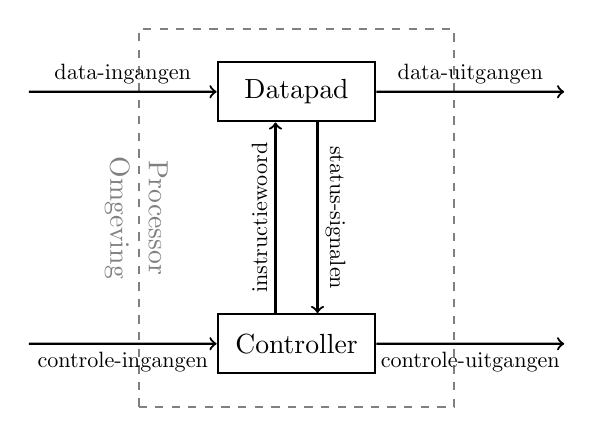
\begin{tikzpicture}[scale=0.8]
\draw[gray,dashed,thick] (-2.5,-3) rectangle (2.5,3);
\draw (-2.5,0) node[rotate=-90,gray,anchor=south]{Processor};
\draw (-2.5,0) node[rotate=-90,gray,anchor=north]{Omgeving};
\node[rectangle,thick,draw=black,minimum width=2 cm,minimum height=0.75 cm] (D) at (0,2) {Datapad};
\node[rectangle,thick,draw=black,minimum width=2 cm,minimum height=0.75 cm] (C) at (0,-2) {Controller};
\draw[->,thick] (D.south -| 0.3333,0) to node[midway,sloped,above,scale=0.8]{status-signalen} (C.north -| 0.3333,0);
\draw[->,thick] (C.north -| -0.3333,0) to node[midway,sloped,above,scale=0.8]{instructiewoord} (D.south -| -0.3333,0);
\draw[<-,thick] (C.west) to node[below,midway,scale=0.8]{controle-ingangen} (-4.25,-2);
\draw[->,thick] (C.east) to node[below,midway,scale=0.8]{controle-uitgangen} (4.25,-2);
\draw[<-,thick] (D.west) to node[above,midway,scale=0.8]{data-ingangen} (-4.25,2);
\draw[->,thick] (D.east) to node[above,midway,scale=0.8]{data-uitgangen} (4.25,2);
\end{tikzpicture}
\label{fig:processorInformationStreams}}
\subfigure[Datapad]{
\begin{tikzpicture}[scale=0.8]
\draw[gray,dashed,thick] (-3.5,-3) rectangle (3.5,3);
\draw (-3.5,1.3) node[rotate=-90,gray,anchor=south]{Datapad};
\draw (-3.5,1.3) node[rotate=-90,gray,anchor=north]{Omgeving};
\node[rectangle,thick,draw=black,minimum width=2 cm] (T) at (0,1.25) {Tijdelijk geheugen};
\node[trapezium,thick,draw=black] (O) at (0,0) {Operatorverbindingen};
\node[rectangle,thick,draw=black,minimum width=2 cm] (F) at (0,-1.25) {Functionele eenheden};
\node[minimum width=2 cm] (RA) at (0,-2.5) {Resultaatverbindingen};
\node[minimum width=2 cm,white] (RB) at (0,2.5) {Resultaatverbindingen};
\draw[thick] (RA.north west) -- (O.bottom left corner |- RA.south) -- (RA.south east) -- ++(1,0) |- (RB.north west) -- (RB.south -| O.bottom left corner) -- (RB.south east) -- ++(0.5,0) |- (RA.north west);
\draw[thick,->] (RB) -- (T);
\draw[thick,->] (T) -- (O);
\draw[thick,->] (O) -- (F);
\draw[thick,->] (F) -- (RA);
\draw[<-,thick] (RA.west -| O.west) -- ++(-3,0);
\draw[<-,thick] (RB.west -| O.west) -- ++(-3,0);
\draw (-4,0) node[scale=0.8,anchor=south]{instructiewoord};
\draw (-4,-2.5) node[scale=0.8,anchor=south]{instructiewoord};
\draw (-4,2.5) node[scale=0.8,anchor=south]{externe-ingangen};
\draw (1.75,-3.5) node[scale=0.8,anchor=south]{externe-uitgangen};
\draw[<-,thick] (O.west) -- ++(-3,0);
\draw[->,thick] (RA) |- ++(3.5,-1);
\end{tikzpicture}
\label{fig:datapadInformationStreams}}
\caption{Opbouw van een processor en datapad.}
\end{figure}
\paragraph{}
Door de controle-ingangen wordt de definitie van ``niet-programmeerbaar'' natuurlijk vaag. We zouden immers het toestandswoord van de controller in grote mate laten afhangen van de invoer die de controle-ingangen. Hierdoor kunnen we de processor toch programmeren. Het onderscheid is dan ook eerder een common-sense.
\subsection{Het Datapad}
Zoals we reeds hebben vermeld, kunnen we een controller modelleren als een eindige toestandsautomaat ofwel finite state machine. Een datapad daarentegen bestaat uit verschillende componenten:
\begin{itemize}
 \item \termen{Functionele Eenheden} ofwel \termen{Functional Units (FU)}: dit zijn schakelingen die berekeningen en aritmetisch operaties uitvoeren. Dit zijn dus de componenten die we in hoofdstuk \ref{ch:combinatoric} hebben besproken: optellers, ALU, schuifoperator,... Uiteraard kunnen we ook zelf functionele eenheden bouwen op de manier die we gezien hebben.
 \item \termen{Tijdelijke geheugens}: dit zijn componenten die de waarden waarop we bewerkingen uitvoeren voor enkele klokcycli kunnen vasthouden. Dit zijn bijvoorbeeld de registerbanken en RAM die we in sectie \ref{s:memoryFSMD} zullen invoeren. Het zijn groepen van flipflops die ons toelaten om op een hoger niveau te redeneren.
 \item \termen{Verbindingen}: de tijdelijke geheugens en de functionele eenheden wisselen informatie uit. Daarom hebben we twee types verbindingen nodig:
 \begin{itemize}
  \item \termen{Operandverbindingen}: dit zijn verbindingen die de waardes van de tijdelijke geheugens overbrengen als operanden van de functionele eenheden. De waarde van een register kan op die manier bijvoorbeeld gebruikt worden bij een optelling.
  \item \termen{Resultaatverbindingen}: het is de bedoeling dat de resultaten vervolgens in een tijdelijk geheugen opgeslagen worden. Resultaatverbindingen transporteren de resultaten van de functionele eenheden terug naar de tijdelijke geheugens. Sommige uitvoer kan ook weggeschreven worden naar de data-uitgangen. Ook de invoer van de data-ingangen wordt door deze verbindingen verwerkt.
 \end{itemize}
 Het spreekt voor zich dat de verbindingen beslissen welke geheugens als operanden en resultaatgeheugens dienen. Daarom zullen we ze implementeren als bussen met multiplexers en 3-state buffers. Deze bussen zullen dan worden aangestuurd door de controller.
\end{itemize}
Dit concept beschrijven we op figuur \ref{fig:datapadInformationStreams}.
\paragraph{}
In het datapad doen we dan ook niets anders dan waardes uit het tijdelijke geheugen inlezen, er een operatie van een functionele eenheid op uitvoeren en vervolgens in een tijdelijk geheugen plaatsen. Dit proces noemen we ook wel de ``\termen{registertransfer}'' en formaliseren we als:
\begin{equation}
\mbox{register}_a\leftarrow\mbox{FU}_a\left(\mbox{register}_{a_1},\mbox{register}_{a_1},\mbox{register}_{a_2},\ldots,\mbox{register}_{a_n}\right)
\end{equation}
In het eerste hoofdstuk hebben we reeds vermeld dat we schakelingen bij het bouwen van een processor beschrijven op registertransfer-niveau. Dit betekent dat we bijvoorbeeld abstractie zullen maken van flipflops en zullen werken met registers. Ook zullen we details als het aantal bits die een opteller nodig heeft verwaarlozen. Deze nieuwe notatiestijl zullen we geleidelijk invoeren.
\section{Formeel Beschrijven van een Algoritme}
\label{s:descriptionFSMD}
Alvorens we een processor kunnen bouwen die een algoritme uitvoert, moeten we eerst een formeel algoritme kunnen opstellen. Dit algoritme vertrekt altijd vanuit een probleemstelling. Hoe we een probleemstelling omzetten naar een algoritme behoort niet tot de inhoud van deze cursus\footnote{Het omzetten van een probleem in een algoritme is geen exacte wetenschap. Het is een vaardigheid die wel geoefend kan worden. Hiervoor bestaan er andere cursussen.}. We zullen altijd stellen dat het algoritme vooraf gekend moet zijn.
\subsection{Leidend Voorbeeld: Deler}
Als leidend voorbeeld doorheen dit hoofdstuk zullen we een processor bouwen die natuurlijke getallen kan delen. Uiteraard zouden we hiervoor een combinatorische schakeling kunnen bouwen. We zullen echter een algoritme beschouwen om de berekening te maken. De processor heeft 2 4-bit ingangen die het deeltal en de deler inlezen. Verder bevat het ook een controle-ingang. Zolang we een laag signaal op de controle-ingang aanleggen betekent dit dat er geen correcte invoer op de data-ingangen staat. Pas wanneer we een hoog signaal aanleggen zal het algoritme dus een deling uitvoeren. Verder bevat de processor ook 2 4-bit uitgang om het quoti\"ent en de rest naar buiten te brengen, en een controle uitgang die hoog wordt op het moment dat het algoritme het quoti\"ent en de rest heeft berekend. Zolang de controle-uitgang dus laag is, is het algoritme nog bezig met de berekening. Verder zal de processor ook wachten totdat de controle-ingang eerst laag is geweest alvorens opnieuw te beginnen. We maken de assumptie dat 
de deler nooit gelijk is aan 0. Het algoritme die dan vervolgens het deeltal en de deler omzet in het quoti\"ent en rest staat op \algoref{alg:devisionFSMD}.
\begin{algorithm}[hbt]
\caption{Delen van twee $n$-bit getallen.}\label{alg:devisionFSMD}
\begin{algorithmic}[1]
\Function{Division}{$N,D$}
\State $Q\gets 0$
\State $R\gets 0$
\For{$I=n-1\mbox{ \textbf{to} }0$}
\State $R\gets R\shlcmd{}1$\Comment{Logische shift $R$ naar links over 1 positie}
\State $R\left[0\right]\gets N\left[n-1\right]$
\State $N\gets N\shlcmd{}1$\Comment{Logische shift $N$ naar links over 1 positie}
\State $Q\gets Q\shlcmd{}1$\Comment{Logische shift $Q$ naar links over 1 positie}
\If{$R\geq D$}
\State $R\gets R-D$
\State $Q\left[0\right]\gets 1$
\EndIf
\EndFor
\State \Return $\left(Q,R\right)$
\EndFunction
\end{algorithmic}
\end{algorithm}
We gaan niet in op de precieze werking van het algoritme. Indien we een index opvragen of zetten bij een variabele zoals $V\left[i\right]$ betekent dit dat we een operatie op de $i$-de bit uitvoeren. We tellen we van rechts naar links, $V[0]$ is dus de minst beduidende bit van $V$ die rechts staat in de encodering. Verder zullen we ook de subscript-notatie gebruiken wanneer we bits samen nemen. Zo betekent $v_2v_1w_2w_2v_2w_1$ dat we een getal samenstellen uit de eerste twee bits van $V$, gevolgd door de eerste en de derde bit van $W$, daarna volgen nog de derde bit van $V$ en de tweede bit van $W$. Dit algoritme is echter niet geschikt voor een processor. Een processor voert immers continu het programma uit. Bovendien wordt hier niet gewacht tot er invoer op de data-ingangen staat. Een laatste opmerking is dat we geen berekeningen op invoer kunnen uitvoeren. Anders zouden we immers de uitgangen van functionele eenheden met de ingangen van de processor verbinden. Daarom dienen we variabelen te introduceren 
die we $X$, $Y$ en $Z$. Daarom zullen we het algoritme herschrijven\footnote{Strikt genomen is dit geen algoritme meer, vermits het nooit eindigt en er geen echt resultaat is. Een betere bewoording is waarschijnlijk procedure.}. We beschouwen hierbij de controle-ingang $ci$ en de controle-uitgang $co$. De herschreven procedure staat in \algoref{alg:devisionFSMDRev}.
\begin{algorithm}[hbt]
\caption{Procedure voor het delen van twee $4$-bit getallen.}\label{alg:devisionFSMDRev}
\begin{algorithmic}[1]
\Procedure{Division}{}
\While{true}
\Repeat\label{algl:s1start}
\State $co\gets 0$
\State $X\gets N$
\State $Y\gets 0$
\State $Z\gets 0$
\Until{$ci$}\label{algl:s1stop}
\For{$I=3\mbox{ \textbf{to} }0$}\label{algl:s2start}
\State $Z\gets Z\shlcmd{}1$\Comment{Logische shift $Z$ naar links over 1 positie}
\State $Z\left[0\right]\gets X\left[3\right]$
\State $X\gets X\shlcmd{}1$\Comment{Logische shift $X$ naar links over 1 positie}
\State $Y\gets Y\shlcmd{}1$\Comment{Logische shift $Y$ naar links over 1 positie}
\If{$Z\geq D$}\label{algl:devisionFSMDComp}
\State $Z\gets Z-D$\label{algl:devisionFSMDSub}
\State $Y\left[0\right]\gets 1$
\EndIf
\EndFor\label{algl:s2stop}
\Repeat\label{algl:s3start}
\State $co\gets 1$
\State $Q\gets Y$
\State $R\gets Z$
\Until{$\neg ci$}\label{algl:s3stop}
\EndWhile
\EndProcedure
\end{algorithmic}
\end{algorithm}
\subsection{Toestandsbeschrijving}
Een eerste probleem dient zich aan hoe we de procedure omzetten in een reeks toestanden. De vraag is immers wat we in \'e\'en zo'n toestand zullen realiseren. Zo kunnen we \algoref{alg:devisionFSMDRev} uitvoeren en per instructie een nieuwe toestand bouwen. Als we echter het programma onder de loep nemen, zien we dat dit algoritme zich uitstekend leent om verschillende instructies samen uit te voeren. Allereerst voeren we in de \textbf{for}-lus hoofdzakelijke shift operaties uit. Deze shiftoperaties vinden plaats over een vast aantal posities. We dienen dus helemaal geen schuifoperator te implementeren, en kunnen eenvoudigweg schuiven met verbindingen. Vervolgens doen we ook aan bitmanipulaties. Omdat deze bitmanipulaties opnieuw op vaste plaatsen plaatsvinden kunnen we dit realiseren met behulp van verbindingen. De enige twee aspecten die enige logica vereisen is de test of $Z\geq D$ is (lijn \ref{algl:devisionFSMDComp}), en het eventueel aftrekken van $D$ uit $Z$ (lijn \ref{algl:devisionFSMDSub}). 
Daarnaast moeten we tijdens de uitvoer van de \textbf{for} lus ook controleren of $I\geq 0$. In dat geval dienen we immers nogmaals de for-lus uit te voeren. We kunnen dit echter controleren met een simpele OR-poort die alle bits van $I$ samenneemt. Indien minstens \'e\'en van de bits een 1 is, zal de OR-lus een 1 teruggeven, en dienen we dus nog een cyclus uit te voeren. Dit leidt ertoe dat we ons algoritme in drie toestanden opdelen:
\begin{enumerate}
 \item $S_0$: inlezen van invoer, initialiseren van variabelen en wachten totdat $ci$ hoog wordt (lijnen \ref{algl:s1start}-\ref{algl:s1stop}).
 \item $S_1$: uitvoeren van een cyclus van de \textbf{for} lus en $I$ met 1 verlagen (lijnen \ref{algl:s2start}-\ref{algl:s2stop}).
 \item $S_2$: resultaten op de uitgang plaatsen en wachten tot $ci$ laag wordt (lijnen \ref{algl:s3start}-\ref{algl:s3stop}).
\end{enumerate}
\subsection{Toestand-Actie Tabel}
Nu we de toestanden hebben vastgesteld kunnen we het algoritme verder formaliseren. Dit zouden we kunnen doen met een grafische voorstelling zoals we gedaan hebben met een eindige toestandsautomaat. Het probleem is dat een rij in het toestandsdiagram niet enkel de voorwaarden en eventuele uitgangen bevat, daarnaast dient het ook nog de acties die door het datapad moeten worden uitgevoerd weer te geven. Dit zou leiden tot een complex en chaotisch diagram. Daarom verkiezen we een tabel: de ``\termen{Toestand-Actie Tabel}''. De tabel bestaat grofweg uit drie gedeeltes:
\begin{itemize}
 \item de huidige toestand: de huidige toestand waarin de controller zich bevindt.
 \item Een toestandsgedeelte: die we kunnen vergelijken met de toestandstabel van een eindige toestandsautomaat. De tabel bevat volgende kolommen:
 \begin{itemize}
  \item condities (afhankelijk van controle- en status-signalen)
  \item de volgende toestand
  \item de uitvoer (van eventuele controle-uitgangen).
 \end{itemize}
 \item een controle-actie gedeelte. Dit gedeelte bevat twee kolommen:
 \begin{itemize}
  \item conditie: een set voorwaarden wanneer een bepaalde set acties (gespecificeerd in de volgende kolom) moet worden uitgevoerd.
  \item actie: afhankelijk van de conditie welke opdrachten uitgevoerd worden op de variabelen in een klokcyclus.
 \end{itemize}
\end{itemize}
Tabel \ref{tbl:stateActionTableRunningExample} toont de toestand-actie tabel van \algoref{alg:devisionFSMDRev}. Een belangrijke opmerking is dat het onderverdelen van toestanden in condities bij het toestandsgedeelte niet verder loopt bij het onderverdelen van diezelfde toestand in het controle-actie gedeelte. Dit betekent dus dat de conditie bij de volgende toestand niet de conditie bij de controle- en datapad-acties impliceert en omgekeerd. Concreet betekent dit dus dat indien $I>0$, dit niet betekent dat $z_2z_1z_0x_3<D$ of dat we de bijbehorende datapad-acties moeten uitvoeren. Het toestandsgedeelte en het controle-actie gedeelte zijn dus onafhankelijk en zijn enkel afhankelijk van de huidige toestand.
\begin{table}[hbt]
\centering
\begin{tabular}{c!{\vrule width 1pt}c|c|c!{\vrule width 1pt}c|c}
Huidige&\multicolumn{2}{c|}{Volgende toestand}&Uit-&\multicolumn{2}{c}{Controle- \& datapad-acties}\\
Toestand&Conditie&Toestand&gang&Conditie&Acties\\\noalign{\hrule height 1pt}
\multirow{4}{*}{$S_0$}&\multirow{2}{*}{$ci=0$}&\multirow{2}{*}{$S_0$}&\multirow{2}{*}{$co=0$}&&$X\gets N$\\
&&&&&$Y\gets 0$\\\cline{2-4}
&\multirow{2}{*}{$ci=1$}&\multirow{2}{*}{$S_1$}&\multirow{2}{*}{$co=0$}&&$Z\gets 0$\\
&&&&&$I\gets 3$\\\noalign{\hrule height 1pt}
\multirow{8}{*}{$S_1$}&\multirow{4}{*}{$I>0$}&\multirow{4}{*}{$S_1$}&\multirow{4}{*}{$co=0$}&\multirow{4}{*}{$z_2z_1z_0x_3<D$}&$Z\gets z_2z_1z_0x_3$\\
&&&&&$X\gets X\shlcmd 1$\\
&&&&&$Y\gets Y\shlcmd 1$\\
&&&&&$I\gets I-1$\\\cline{2-6}
&\multirow{4}{*}{$I=0$}&\multirow{4}{*}{$S_2$}&\multirow{4}{*}{$co=0$}&\multirow{4}{*}{$z_2z_1z_0x_3\geq D$}&$Z\gets z_2z_1z_0x_3-D$\\
&&&&&$X\gets X\shlcmd 1$\\
&&&&&$Y\gets y_2y_1y_01$\\
&&&&&$I\gets I-1$\\\noalign{\hrule height 1pt}
\multirow{6}{*}{$S_2$}&\multirow{3}{*}{$ci=0$}&\multirow{3}{*}{$S_0$}&$co=1$&&\\
&&&$Q=Y$&&\\
&&&$R=Z$&&\\\cline{2-4}
&\multirow{3}{*}{$ci=1$}&\multirow{3}{*}{$S_2$}&$co=1$&&\\
&&&$Q=Y$&&\\
&&&$R=Z$&&\\
\end{tabular}
\caption{Toestand-actie tabel van het leidend voorbeeld.}
\label{tbl:stateActionTableRunningExample}
\end{table}
\paragraph{Simulatie}Om ons meer vertrouwd te maken met het concept van een toestand-actie tabel zullen we een deling simuleren met behulp van de tabel. We zullen $N=12$ delen door $D=7$ op de processor en stap per stap kijken wat er verandert. Dit doen we met behulp van tabel \ref{tbl:stateActionTableRunningExampleSim}. Omdat we met bitoperaties werken zullen we alle variabelen in de tabel in binaire notatie zetten.
\begin{table}[hbt]
\centering
\begin{tabular}{c|c|c|c}
Toestand&Voldane Condities&Acties&Uitvoer\\\hline
\multirow{4}{*}{$S_0$}&\multirow{4}{*}{$ci=1$}&$X\gets N=1100$&\multirow{4}{*}{$co=0$}\\
&&$Y\gets0000$&\\
&&$Z\gets0000$&\\
&&$I\gets11$&\\\hline

\multirow{4}{*}{$S_1$}&\multirow{2}{*}{$I=11>00$}&$Z\gets z_2z_1z_0x_3=0001$&\multirow{4}{*}{$co=0$}\\
&&$X\gets X\shlcmd{} 1=1000$&\\
&\multirow{2}{*}{$z_2z_1z_0x_3=0001<D=0101$}&$Y\gets Y\shlcmd{} 1=0000$&\\
&&$I\gets I-1=10$&\\\hline

\multirow{4}{*}{$S_1$}&\multirow{2}{*}{$I=10>00$}&$Z\gets z_2z_1z_0x_3=0011$&\multirow{4}{*}{$co=0$}\\
&&$X\gets X\shlcmd{} 1=0000$&\\
&\multirow{2}{*}{$z_2z_1z_0x_3=0011<D=0101$}&$Y\gets Y\shlcmd{} 1=0000$&\\
&&$I\gets I-1=01$&\\\hline

\multirow{4}{*}{$S_1$}&\multirow{2}{*}{$I=01>00$}&$Z\gets z_2z_1z_0x_3-D=0001$&\multirow{4}{*}{$co=0$}\\
&&$X\gets X\shlcmd{} 1=0000$&\\
&\multirow{2}{*}{$z_2z_1z_0x_3=0110\geq D=0101$}&$Y\gets y_2y_1y_01=0001$&\\
&&$I\gets I-1=00$&\\\hline

\multirow{4}{*}{$S_1$}&\multirow{2}{*}{$I=00$}&$Z\gets z_2z_1z_0x_3=0010$&\multirow{4}{*}{$co=0$}\\
&&$X\gets X\shlcmd{} 1=0000$&\\
&\multirow{2}{*}{$z_2z_1z_0x_3=0010<D=0101$}&$Y\gets Y\shlcmd{} 1=0010$&\\
&&$I\gets I-1=11$&\\\hline

\multirow{3}{*}{$S_2$}&\multirow{3}{*}{$ci=0$}&&$co=1$\\
&&&$Q=Y=0010$\\
&&&$R=Z=0010$\\
\end{tabular}
\caption{Simulatie van het algoritme met behulp van de toestand-actie tabel (tabel \ref{tbl:stateActionTableRunningExample}).}
\label{tbl:stateActionTableRunningExampleSim}
\end{table}
We stellen dat vanaf dat we de simulatie beginnen, reeds de data reeds op de ingangen van de processor aangelegd staat. Bijgevolg is $ci=1$, $N=1100$ en $D=0101$. We maken verder ook een assumptie dat $X$, $Y$ en $Z$ 4-bit geheugens zijn, dit is redelijk vermits we uitsluitend bits in dit bereik gebruiken, en we geen schuifoperaties naar rechts uitvoeren waardoor hogere bits in het bereik zouden komen te liggen. $I$ is een 2-bit geheugen vermits het uitsluitend waardes tussen 0 en 3 moet aannemen. Initieel vertrekt de processor vanuit toestand $S_0$ we zien op die toestand-actie tabel dat in toestand $S_0$ de ingangen in de geheugens worden ingelezen. Vermits er data op de ingangen staat, krijgt $X$ de waarde van de teller $N=1100$. De overige variabelen worden ge\"initialiseerd zoals beschreven staat in de toestand-actie tabel. Omdat $ci=1$ kunnen we afleiden dat de volgende toestand $S_1$ is. Verder specificeert de tabel ook dat we een laag signaal op de controle-uitgang moeten aanleggen (momenteel staat 
er immers geen uitkomst op de uitgangen). In de volgende stap bevinden we ons in toestand $S_1$. We evalueren eerst de verschillende condities ??.
\subsection{ASM-Schema}
Zoals reeds gezegd is de visualisatie van een eindige toestandsautomaat niet toereikend om een algoritme weer te geven. Een grafisch voorstelling die we wel kunnen gebruiken is een ``\termen{Algorithmic-State-Machine Chart}'' ofwel ``\termen{ASM-schema}''.
\subsubsection{ASM-Elementen}
Een ASM-schema lijkt op een flow-chart en bestaat drie verschillende soorten ``\termen{ASM-elementen}'':
\begin{itemize}
 \item \termen{Toestandskader} ofwel \termen{state box}: dit is een set niet-conditionele toekenning. We stellen een toestandskader voor door middel van een rechthoek waarin we de toekenningen schrijven. De toekenningen in \'e\'en toestandskader worden parallel uitgevoerd. Daarnaast bevat een toestandskader ook de status- en data-uitgangen van de processor. Men maakt een onderscheid doordat toekenningen met een pijl ($\gets$) weergegeven worden en uitgangen met een gelijkheidsteken ($=$). Figuur \ref{fig:asmElementState} toont een voorbeeld van een toestandskader.
 \item \termen{Beslissingskader} ofwel \termen{decision box}: dit is de voorstelling van een bepaalde conditie. Een conditie wordt voorgesteld met behulp van een ruit, waarin de conditie wordt geschreven. Vanuit een beslissingskader vertrekken er twee pijlen: voor het geval waarin de voorwaarde waar of vals is. We noteren de pijlen dan ook respectievelijk met ``[True]'' en ``[False]'', soms wordt ook 1 en 0 gebruikt. Figuur \ref{fig:asmElementDecision} toont een voorbeeld van een beslissingskader.
 \item \termen{Conditioneel kader} ofwel \termen{conditional box}: Dit is een toestandskader die enkel onder voorwaarden gespecificeerd door een beslissingskader worden uitgevoerd. Ook deze toekenningen worden in parallel uitgevoerd. Verder bevat een conditioneel kader ook de conditionele uitvoer op de processoruitgangen. We noteren toekenningen en uitgangen op dezelfde manier als bij toestandskaders. Men stelt een conditioneel kader voor als een rechthoek met afgeronde hoeken. Figuur \ref{fig:asmElementConditional} toont een voorbeeld van een conditioneel kader.
\end{itemize}
\begin{figure}[hbt]
\centering
\subfigure[Toestandskader]{
\begin{tikzpicture}
%\node[asmS] (S) at (0,0) {$\begin{array}{c}\mbox{niet conditioneel commando 1}\\\mbox{niet conditioneel commando 2}\\\cdots\\\mbox{niet conditioneel commando $n$}\end{array}$};
\node[asmS] (S) at (0,0) {$\begin{array}{c}\mbox{variabele$_1\gets$ expressie$_1$}\\\cdots\\\mbox{variabele$_m\gets$ expressie$_m$}\\\mbox{uitgang$_1=$ expressie$_{m+1}$}\\\cdots\\\mbox{uitgang$_n=$ expressie$_{m+n}$}\end{array}$};
\draw[<-] (S) -- ++(0,1.5) node[anchor=south]{in};
\draw[->] (S) -- ++(0,-1.5) node[anchor=north]{uit};
\end{tikzpicture}
\label{fig:asmElementState}
}
\subfigure[Beslissingskader]{
\begin{tikzpicture}
\node[asmD] (D) at (0,0) {test};
\draw[<-] (D) -- ++(0,1.5) node[anchor=south]{in};
\draw[->] (D) -| ++(-1.75,-1.5) node[anchor=north]{uit 1};
\draw[->] (D) -| ++(1.75,-1.5) node[anchor=north]{uit 2};
\draw (-1.75,0) node[anchor=south west,scale=0.75]{[True]};
\draw (1.75,0) node[anchor=south east,scale=0.75]{[False]};
\end{tikzpicture}
\label{fig:asmElementDecision}
}
\subfigure[Conditioneel kader]{
\begin{tikzpicture}
%\node[asmC] (C) at (0,0) {$\begin{array}{c}\mbox{conditioneel commando 1}\\\mbox{conditioneel commando 2}\\\cdots\\\mbox{conditioneel commando $n$}\end{array}$};
\node[asmC] (C) at (0,0) {$\begin{array}{c}\mbox{variabele$_1\gets$ expressie$_1$}\\\cdots\\\mbox{variabele$_m\gets$ expressie$_m$}\\\mbox{uitgang$_1=$ expressie$_{m+1}$}\\\cdots\\\mbox{uitgang$_n=$ expressie$_{m+n}$}\end{array}$};
\draw[<-] (C) -- ++(0,1.5) node[anchor=south]{in};
\draw[->] (C) -- ++(0,-1.5) node[anchor=north]{uit};
\end{tikzpicture}
\label{fig:asmElementConditional}
}
\caption{Voorstelling van de verschillende ASM-elementen}
\label{fig:asmElementsEnum}
\end{figure}
\subsubsection{Het ASM-Blok}
Deze ASM-elementen worden gegroepeerd in een ``\termen{ASM-blok}''. Alle ASM-elementen die in eenzelfde ASM-blok zitten, worden dan in \'e\'en klokcyclus uitgevoerd. Hierdoor voorzien we per toestand in de Toestand-Actie tabel een ASM-blok. Het blok zelf moet dan specificeren wat er in de toestand gebeurt. We zullen dit component voorstellen met behulp van een vierkant met streepjeslijnen. Vermits alle acties in \'e\'en klokflank uitgevoerd worden, bevat elk ASM-blok exact \'e\'en toestandskader. Dit toestandskader bevat dan alle toekenningen en uitgangen die onafhankelijk van condities in die toestand worden uitgevoerd. Indien er geen onafhankelijke operaties zijn, is het vierkant leeg. Indien er naast onafhankelijke acties ook onafhankelijk acties gebeuren (zowel in het toestand- als het actie-gedeelte), zullen we vervolgens enkele beslissingskaders plaatsen. We voeren testen uit op variabelen in het datapad door middel van status-signalen en eventuele signalen aan de controle-ingangen. Vermits we al deze 
testen reeds in de toestand-actie-tabel hebben gedefinieerd kunnen we eenvoudig de toestand-actie-tabel omvormen tot een ASM-schema. Zo staat op figuur \ref{fig:aSMSchemaRunningExample} het ASM-schema voor het leidend voorbeeld.
\begin{figure}[hbt]
\centering
\begin{tikzpicture}
\def\ds{6};
\def\di{1.75};
\def\dy{-2};
\def\offset{1};
\node[asmS] (S1S) at (0,0) {$\begin{array}{c}X\gets N\\Y\gets 0\\Z\gets 0\\I\gets 3\\co=0\end{array}$};
\node[asmD] (S1D) at (0,\dy) {$ci=0$};
\draw[->] (S1S) -- (S1D);
\draw[->] (S1D) -| (-\di,0) -- (S1S);
\setTrueFalseLabels{S1D};

\node[asmS] (S2S) at (\ds,0) {$\begin{array}{c}X\gets X\shlcmd 1\\I\gets I-1\\co=0\end{array}$};
\node[asmD] (S2D1) at (\ds,\dy) {$z_2z_1z_0x_3<D$};
\draw[->] (S2S) -- (S2D1);
\node[asmC] (S2C1) at (\ds-\di,2*\dy) {$\begin{array}{c}Z\gets z_2z_1z_0x_3\\Y\gets Y\shlcmd{} 1\end{array}$};
\draw[->] (S2D1) -| (S2C1);
\node[asmC] (S2C2) at (\ds+\di,2*\dy) {$\begin{array}{c}Z\gets z_2z_1z_0x_3-D\\Y\gets y_2y_1y_01\end{array}$};
\draw[->] (S2D1) -| (S2C2);
\draw (S2C1) |- (\ds,2.5*\dy) -| (S2C2);
\node[asmD] (S2D2) at (\ds,3*\dy) {$I>0$};
\draw[->] (\ds,2.5*\dy) -- (S2D2);
\draw[->] (S1D) -| (\di,\offset) -| (S2S);
\draw[->] (S2D2) -| (\ds-2*\di,0) -- (S2S);
\setTrueFalseLabels{S2D1};
\setTrueFalseLabels{S2D2};

\node[asmS] (S3S) at (2*\ds,0) {$\begin{array}{c}co=1\end{array}$};
\node[asmD] (S3D) at (2*\ds,\dy) {$ci=1$};
\node[asmN] (N1) at (2*\ds,2*\dy) {$\begin{array}{c}Q=Y\\R=Z\end{array}$};
\draw[->] (S2D2) -| (\ds+2*\di,\offset) -| (S3S);
\draw[->] (S3S) -- (S3D);
\draw[->] (S3D) -| (2*\ds-\di,0) -- (S3S);
\draw[->] (S3D) -| (\di+2*\ds,1.5) -| (S1S);
\setTrueFalseLabels{S3D};
\begin{pgfonlayer}{background}
\node[asmB, fit=(S1S) (S1D)] (S1) {};
\node[asmB, fit=(S2S) (S2D1) (S2D2) (S2C1) (S2C2)] (S2) {};
\node[asmB, fit=(S3S) (S3D)] (S3) {};
\end{pgfonlayer}
\draw (S1.south west) node[anchor=south west]{$S_1$};
\draw (S2.south west) node[anchor=south west]{$S_2$};
\draw (S3.south west) node[anchor=south west]{$S_3$};
\end{tikzpicture}
\caption{ASM-schema van het leidend voorbeeld.}
\label{fig:aSMSchemaRunningExample}
\end{figure}
\subsubsection{Traditionele Valkuilen}
Traditioneel maakt men een aantal fouten tegen ASM-schemas. In deze subsubsectie zullen we een overzicht geven van de meest gemaakte fouten.
\begin{figure}[hbt]
\centering
\subfigure[Meerdere volgende toestanden]{
\begin{tikzpicture}
\node[asmS] (A0) at (0,0) {$A_0$};
\node[asmD] (T0) at (-1.75,-1.25) {$t_1$};
\node[asmD] (T1) at (1.75,-1.25) {$t_2$};
\node[asmS] (A1) at (-3,-2.375) {$A_1$};
\node[asmS] (A2) at (0,-2.375) {$A_2$};
\node[asmS] (A3) at (3,-2.375) {$A_3$};
\setTrueFalseLabels{T0};
\setTrueFalseLabels{T1};
\draw[->] (A0) -- (0,-0.5) -| (T0);
\draw[->] (0,-0.5) -| (T1);
\draw[->] (T0) -| (A1);
\draw[->] (T1) -| (A3);
\draw[->] (T0) -| (A2);
\draw[<-] (A0) -- ++(0,0.75);
\draw (T1) -| (0,-1.25);
\pdot{0,-0.5};
\pdot{0,-1.25};
\begin{pgfonlayer}{background}
\node[asmB, fit=(A0) (T0) (T1)] (S1) {};
\node[asmB, fit=(A1)] (S2) {};
\node[asmB, fit=(A2)] (S3) {};
\node[asmB, fit=(A3)] (S4) {};
\end{pgfonlayer}
\draw (S1.south west) node[anchor=south west]{$S_1$};
\draw (S2.south west) node[anchor=south west]{$S_2$};
\draw (S3.south west) node[anchor=south west]{$S_3$};
\draw (S4.south west) node[anchor=south west]{$S_4$};
\end{tikzpicture}
\label{fig:badASMMultipleFlows}
}
\subfigure[Geen volgende toestanden]{
\begin{tikzpicture}
\node[asmS] (A0) at (0,0) {$A_0$};
\node[asmD] (T0) at (0,-1.25) {$t_1$};
\node[asmS] (A1) at (1.25,-2.375) {$A_1$};
\setTrueFalseLabels{T0};
\draw[->] (A0) -- (T0);
\draw[->] (T0) -| (A1);
\draw[<-] (A0) -- ++(0,0.75);
\draw (T0) -| (-1.25,-0.5) -- (0,-0.5);
\pdot{0,-0.5};
\begin{pgfonlayer}{background}
\node[asmB, fit=(A0) (T0)] (S1) {};
\node[asmB, fit=(A1)] (S2) {};
\end{pgfonlayer}
\draw (S1.south west) node[anchor=south west]{$S_1$};
\draw (S2.south west) node[anchor=south west]{$S_2$};
\end{tikzpicture}
\label{fig:badASMNoFlows}
}
\subfigure[Meerdere toekenningen]{
\begin{tikzpicture}
\node[asmS] (A0) at (0,0) {$X\gets 0$};
\node[asmD] (T0) at (0,-0.75) {$t_1$};
\node[asmC] (A1) at (1.25,-1.5) {$X\gets 1$};
\node[asmS] (A2) at (0,-2.5) {$A_0$};
\setTrueFalseLabels{T0};
\draw[->] (A0) -- (T0);
\draw[->] (T0) -| (A1);
\draw[<-] (A0) -- ++(0,0.75);
\draw[->] (T0) -| (-1.25,-2) -| (A2);
\draw (A1) |- (0,-2);
\pdot{0,-2};
\begin{pgfonlayer}{background}
\node[asmB, fit=(A0) (T0) (A1)] (S1) {};
\node[asmB, fit=(A2)] (S2) {};
\end{pgfonlayer}
\draw (S1.south west) node[anchor=south west]{$S_1$};
\draw (S2.south west) node[anchor=south west]{$S_2$};
\end{tikzpicture}
\label{fig:badASMMultipleAssignments}
}
\subfigure[Testen op nieuwe waarden]{
\begin{tikzpicture}
\node[asmS] (A0) at (0,0.25) {$a\gets a-1$};
\node[asmD] (T0) at (0,-0.75) {$a>3$};
\node[asmC] (A1) at (-1.25,-1.5) {$b\gets 2$};
\node[asmS] (A2) at (0,-2.5) {$A_0$};
\setTrueFalseLabels{T0};
\draw[->] (A0) -- (T0);
\draw[->] (T0) -| (A1);
\draw[<-] (A0) -- ++(0,0.75);
\draw[->] (T0) -| (1.25,-2) -| (A2);
\draw (A1) |- (0,-2);
\pdot{0,-2};
\begin{pgfonlayer}{background}
\node[asmB, fit=(A0) (T0) (A1)] (S1) {};
\node[asmB, fit=(A2)] (S2) {};
\end{pgfonlayer}
\draw (S1.south west) node[anchor=south west]{$S_1$};
\draw (S2.south west) node[anchor=south west]{$S_2$};
\end{tikzpicture}
\label{fig:badASMTests}
}
\subfigure[Gebruik nieuwe waarde]{
\begin{tikzpicture}
\node[asmS] (A00) at (0,0) {$y\gets x+1$};
\node[asmS] (A01) at (0,-1) {$z\gets y+2$};
\draw[->] (0,0.75) -- (A00);
\draw[->] (A00) -- (A01);
\draw[->] (A01) -- (0,-1.75);
\node (A) at (1.5,-0.5) {$\neq$};
\node[asmS] (A1) at (3,-0.5) {$\begin{array}{c}y\gets x+1\\z\gets y+2\end{array}$};
\draw[->] (3,0.75) -- (A1);
\draw[->] (A1) -- (3,-1.75);
\end{tikzpicture}
\label{fig:badASMUsage}
}
\subfigure[Conditioneel na toestandskader]{
\begin{tikzpicture}
\node[asmS,minimum width=3cm] (A00) at (0,0) {$A_0$};
\node[asmC,minimum width=3cm] (A01) at (0,-1) {$A_1$};
\draw[->] (0,0.75) -- (A00);
\draw[->] (A00) -- (A01);
\draw[->] (A01) -- (0,-1.75);
\end{tikzpicture}
\label{fig:badCAfterS}
}
\subfigure[Toewijzen uitgang]{
\begin{tikzpicture}
\node[asmS] (A1) at (3,-0.5) {$\mbox{uitgang}\gets\mbox{expressie}$};
\draw[->] (3,0.75) -- (A1);
\draw[->] (A1) -- (3,-1.75);
\end{tikzpicture}
}
\caption{Traditionele valkuilen bij het maken van ASM-schema's.}
\label{fig:badASM}
\end{figure}
\paragraph{Meerdere volgende toestanden}Men kan in een ASM-schema een flow chart tekenen waarbij onder bepaalde condities, men twee verschillende pijlen kan volgen. Een voorbeeld van zo'n flow chart staat op figuur \ref{fig:badASMMultipleFlows}. Indien bijvoorbeeld test $t_1$ slaagt en $t2$ faalt, dienen we de stromen naar $A_1$ \'en $A_3$ te volgen. Dit is niet zo problematisch wanneer dit in hetzelfde ASM-blok gebeurd (we kunnen argumenteren dat we dan alle toewijzingen uit $A_1$ en $A_3$ uitvoeren). Indien we echter later naar verschillende toestanden gaan krijgen we problemen. We kunnen dit probleem makkelijk verhelpen door geen vertakkingen met pijlen toe te staan. Enkel uit het beslissingskader vertrekken twee pijlen. Uit een toestands- en conditioneel kader vertrekt altijd slechts \'e\'en pijl. Het samenbrengen van pijlen is wel toegelaten.
\paragraph{Geen volgende toestand}Ook het omgekeerde kan voorkomen: een ASM-blok waarbij we geen volgende toestand bekomen bij een bepaalde situatie. Figuur \ref{fig:badASMNoFlows} toont een minimaal voorbeeld: indien aan $t_1$ wordt voldaan zullen we nooit naar een volgende toestand overgaan. Dit komt omdat de pijl nooit een toestandskader bereikt (en we dus in een volgende toestand komen. Ook dit probleem kunnen we eenvoudig voorkomen: in elk ASM-blok gaan alle mogelijke lussen doorheen het toestandskader.
\paragraph{Verschillende toekenningen aan dezelfde variabele} Tijdens \'e\'en klokflank kan een variabele slechts \'e\'enmaal van waarde veranderen. We kunnen in een ASM-blok echter meerdere kaders plaatsen die elk een waarde aan dezelfde variabele toekennen. Figuur \ref{fig:badASMMultipleAssignments} toont zo'n situatie: indien $t_1$ niet waar is, kennen we zowel $0$ als $1$ toe aan $X$. Men kan argumenteren dat $X$ dan de waarde $1$ krijgt, omdat dit de laatste toekenning is aan $X$ in het diagram. De componenten die in een ASM-blok staan kunnen dus vrij verandert worden in volgorde. Bovendien zullen we in sectie \ref{s:syntheseFSMD} een mechanisme ontwikkelen om deze ASM-schema's om te zetten in hardware. Incorrecte ASM-schema's zullen leiden tot implementatiefouten. We kunnen dit voorkomen door bij elk ASM-blok alle mogelijke paden te analyseren en te controleren dat geen variabele twee toewijzingen krijgt.
\paragraph{Testen van nieuwe waarde} Omdat alles in een ASM-blok tegelijk gebeurt zijn de waardes van variabelen ook nog niet aangepast wanneer we een toestandsblok verlaten. Zolang we ons echter nog in hetzelfde ASM-blok bevinden, zijn die aanpassingen nog niet doorgevoerd. Stel dat we bijvoorbeeld volgende \texttt{C} programma beschouwen:
\begin{verbatim}
a--;
if(a > 3) {
  b = 2;
}
\end{verbatim}
Dan kunnen we dit vertalen naar \'e\'en toestand in het ASM-schema. Figuur \ref{fig:badASMTests} is echter niet de juiste vertaling. Stel immers dat $a=4$ dan zal in het \texttt{C}-programma de \texttt{if}-lus niet uitgevoerd worden, $a$ heeft immers voor het \texttt{if}-statement de waarde $3$. In het ASM-schema krijgt $a$ ook de waarde $3$, maar alleen nadat we het ASM-blok verlaten hebben. Bijgevolg zal bij de voorwaarde $a$ nog steeds de waarde $4$ hebben. En zal de \texttt{if}-lus uitgevoerd worden. Een oplossing is om in dit geval gewoon te testen op $a-1>3$ of dus $a>4$.
\paragraph{Gebruiken van een nieuwe waarde} Een verwante traditionele fout is het gebruiken van de nieuwe waarde in de volgende berekening. Een voorbeeld van dit concept staat op figuur \ref{fig:badASMUsage}. Hier zien we twee ASM-schema's die niet equivalent zijn. Indien bijvoorbeeld $x=2$ en $y=1$ zal in de eerste flow $z=5$. In het tweede geval is $z=3$. Indien beide kaders in een verschillend ASM-blok of -element staan, is dit uiteraard toegelaten. Indien de toekenningen in hetzelfde ASM-element of ASM-blok staan, worden de opdrachten parallel uitgevoerd, en zullen we dus de oude waarde gebruiken. Men kan dit fenomeen testen door de volgorde van toekenningen in een ASM-element te wijzigen of de beslissingskaders en hun bijbehorende conditionele kaders anders te schikken. Nadat deze volgorde dan wijzigt, zou het programma nog steeds op dezelfde manier moeten werken.
\paragraph{Aanduiden van controller-uitgangen}We zijn reeds kort ingegaan op de notatie van uitgangen in de toestand- en conditionele kaders. We noteren de waarde van een uitgang met behulp van een gelijkheidsteken ($=$). Indien we de uitgang niet vermelden, staat er een 0 op die uitgang (in het geval van meerdere bits, zijn alle bits dus 0). Soms komt het ook voor dat een uitgang in elke toestand een combinatorische schakeling van enkele variabelen is. In dat geval moeten we deze uitgang niet in elk toestandskader vermelden, maar volstaat het om een nota te maken, zoals we ook op figuur \ref{fig:aSMSchemaRunningExample}. Deze nota is geen onderdeel van het ASM-schema, en wordt makkelijk vergeten.
\paragraph{Conditioneel kader na toestandskader}Een laatste fout die regelmatig terugkomt is het plaatsen van een conditioneel kader na een toestandskader zoals op figuur \ref{fig:badCAfterS}. Vermits er geen beslissingskader aan vooraf gaat, is dit conditioneel kader helemaal niet gebonden aan een voorwaarde. Dit probleem lossen we op door het conditioneel kader om te vormen tot een toestandskader. Indien beide kaders bovendien in eenzelfde ASM-blok staan, kunnen we de inhoud van beide kaders samennemen in \'e\'en toestandskader.
\subsubsection{Inputgebaseerde en Toestandsgebaseerde ASM-schema's}
We hebben het reeds kort gehad over het toekennen van toestanden aan delen van een programma besproken. Een belangrijk aspect daarbij is dat we ASM-schema's kunnen onderverdelen in twee categorie\"en:
\begin{itemize}
 \item \termen{Inputgebaseerd ASM-schema}: In dit schema kunnen we de waarde van testen (status-signale) en controle-ingangen onmiddellijk gebruiken. Een inputgebaseerd ASM-schema van het leidend voorbeeld stond op figuur \ref{fig:aSMSchemaRunningExample}.
 \item \termen{Toestandsgebaseerd ASM-schema}: Hierbij kunnen we de waardes van testen (status-signalen) en controle-ingangen pas in de volgende klokflank gebruiken. Het betekent dus dat elke voorwaardelijke uitvoering van een opdracht gepaard gaat met de overgang naar een nieuwe toestand. Bijgevolg bevat dit diagram ook geen conditionele kaders.
\end{itemize}
Inputgebaseerde ASM-schema's kunnen meer opdrachten uitvoeren in een klokflank, omdat we niet moeten wachten op het kloksignaal om conditionele operaties uit te voeren. Anderzijds zal dit ASM-schema tot een langere klokcyclus leiden. Dit komt omdat de testen eerst moeten berekend worden alvorens we sommige opdrachten kunnen uitvoeren. Een nadeel van toestandsgebaseerde ASM-schema's is dat we meer toestanden nodig hebben, wat zal leiden tot een groter geheugen en mogelijk ook logica.
\paragraph{}
De termen inputgebaseerd en toestandsgebaseerd komen van de controller. We hebben reeds besproken dat een controller een eindige toestandsautomaat is. Ook bij deze eindige toestandsautomaten hebben we deze indeling gemaakt. Een toestandsgebaseerd ASM-schema zal aanleiding geven tot een toestandsgebaseerde controller en vice versa. Bij wijze van voorbeeld zullen we het leidend voorbeeld ook met een toestandsgebaseerd ASM-schema visualiseren op figuur \ref{fig:aSMSchemaRunningExampleState}.
\begin{figure}[hbt]
\centering
\begin{tikzpicture}
\def\ds{6};
\def\di{1.75};
\def\dy{-2};
\def\offset{1};
\node[asmS] (S1S) at (0,0) {$\begin{array}{c}X\gets N\\Y\gets 0\\Z\gets 0\\I\gets 3\\co=0\end{array}$};
\node[asmD] (S1D) at (0,\dy) {$ci=0$};
\draw[->] (S1S) -- (S1D);
\draw[->] (S1D) -| (-\di,0) -- (S1S);
\setTrueFalseLabels{S1D};

\node[asmS] (S2S) at (\ds,0) {$\begin{array}{c}X\gets X\shlcmd 1\\co=0\end{array}$};
\node[asmD] (S2D1) at (\ds,\dy) {$z_2z_1z_0x_3<D$};
\draw[->] (S2S) -- (S2D1);
\node[asmS] (S4S) at (\ds-\di,2*\dy) {$\begin{array}{c}Z\gets z_2z_1z_0x_3\\I\gets I-1\\Y\gets Y\shlcmd{} 1\end{array}$};
\draw[->] (S2D1) -| (S4S);
\node[asmS] (S5S) at (\ds+\di,2*\dy) {$\begin{array}{c}Z\gets z_2z_1z_0x_3-D\\I\gets I-1\\Y\gets y_2y_1y_01\end{array}$};
\draw[->] (S2D1) -| (S5S);
\node[asmD] (S4D) at (\ds-\di,3*\dy) {$I>0$};
\draw[->] (S4S) -| (S4D);
\node[asmD] (S5D) at (\ds+\di,3*\dy) {$I>0$};
\draw[->] (S5S) -| (S5D);
\draw[->] (S1D) -| (\di,\offset) -| (S2S);
\draw[->] (S4D) -| (\ds-2*\di,0) -- (S2S);
\setTrueFalseLabels{S2D1};
\setTrueFalseLabels{S4D};
\setTrueFalseLabels{S5D};

\node[asmS] (S3S) at (2*\ds,0) {$\begin{array}{c}co=1\end{array}$};
\node[asmD] (S3D) at (2*\ds,\dy) {$ci=1$};
\node[asmN] (N1) at (2*\ds,2*\dy) {$\begin{array}{c}Q=Y\\R=Z\end{array}$};
\draw[->] (S4D) -| (\ds-0.375*\di,3.75*\dy) -| (\ds+2*\di,\offset) -| (S3S);
\draw (S5D) -| (\ds+0.375*\di,3.5*\dy) -| (\ds-2*\di,0 |- S4D);
\draw (S5D) -- (S5D -| \ds+2*\di,0);
\pdot{S5D -| \ds+2*\di,0}
\pdot{\ds-2*\di,0 |- S4D}
\draw[->] (S3S) -- (S3D);
\draw[->] (S3D) -| (2*\ds-\di,0) -- (S3S);
\draw[->] (S3D) -| (\di+2*\ds,1.5) -| (S1S);
\setTrueFalseLabels{S3D};
\begin{pgfonlayer}{background}
\node[asmB, fit=(S1S) (S1D)] (S1) {};
\node[asmB, fit=(S2S) (S2D1)] (S2) {};
\node[asmB, fit=(S3S) (S3D)] (S3) {};
\node[asmB, fit=(S4S) (S4D)] (S4) {};
\node[asmB, fit=(S5S) (S5D)] (S5) {};
\end{pgfonlayer}
\draw (S1.south west) node[anchor=south west]{$S_1$};
\draw (S2.south west) node[anchor=south west]{$S_2$};
\draw (S3.south west) node[anchor=south west]{$S_3$};
\draw (S5.south west) node[anchor=south west]{$S_4$};
\draw (S4.south west) node[anchor=south west]{$S_5$};
\end{tikzpicture}
\caption{Toestandsgebaseerd ASM-schema van het leidend voorbeeld.}
\label{fig:aSMSchemaRunningExampleState}
\end{figure}
\section{Geheugencomponenten}
\label{s:memoryFSMD}
Alvorens we processoren kunnen implementeren zullen we eerst nieuwe componenten moeten introduceren. We zullen we deze componenten introduceren in een logische volgorde waarbij componenten gebruik maken van eerder ge\"introduceerde componenten.
\subsection{Register File Cell (RFC)}
Een \termen{register file cell} is een uitbreiding op een geklokte D-flipflop. Het component bevat een klok-ingang $\mbox{Clk}$, data-ingangen $D_{\mbox{\small{in}}1},\ldots,D_{\mbox{\small{in}}m}$, data-uitgangen $D_{\mbox{\small{out}}1},\ldots,D_{\mbox{\small{out}}n}$, \termen{leespoorten $\mbox{RE}_1,\mbox{RE}_{n}$} (ook wel ``\termen{Read-Enabled}'' genoemd) en \termen{schrijfpoorten $\mbox{WE}_1,\ldots,\mbox{WE}_{\left\lceil\log_2m+1\right\rceil}$} (ook wel ``\termen{Write-Enabled}'' genoemd). Deze ingangen laten ons toe om te kiezen uit welke data-ingang we data willen inlezen en deze bij de klokflank willen opslaan. We zullen data geklokt wegschrijven, net zoals bij een D-flipflop. Indien alle schrijfpoorten $\mbox{WE}_i=0$ lezen we geen nieuwe waarde in, en blijft de oude waarde behouden. In de andere gevallen dienen de schrijfpoorten een binaire getal $a$ te bepalen vanuit welke data-ingang $d_{\mbox{\small{in}}a}$ we data inlezen. Indien er voor het aantal data-ingangen $m$ geen natuurlijk getal 
$l$ bestaat zodat $l=\log_2 m+1$, zal er bij alle overige write-enable configuraties, data ingelezen worden uit de laatste data-ingang. Daarnaast kunnen we op eender welke uitgang de inhoud van het geheugen plaatsen. Vandaar dat er per uitgang ook een read-enable ingang is voorzien. Indien we een laag signaal aanleggen op een read-enable ingang $\mbox{RE}_i$, zal de overeenkomstige uitgang $D_{\mbox{\small{out}}i}$ hoog impedant zijn. De toestand van de uitgangen is niet geklokt: indien we tijdens twee klokflanken in een read-enable ingang aanpassen zullen we mits enige vertraging het resultaat op de data-uitgang zien, we hoeven dus niet op een klokflank te wachten. Op figuur \ref{fig:registerFileCell} tonen we een implementatie van een Register File Cell met $m=n=2$.
\begin{figure}[hbt]
\centering
\begin{tikzpicture}
\node[dff] (D) at (0,0) {};
\node[mux4to1,rotate=90] (M) at (-1.75,0 |- D.D) {};
\draw (M.output) -- (D.D);
\node[tris] (T1) at (1.75,0 |- D.Q) {};
\node[tris] (T2) at (2.5,-0.25) {};
\draw (D.Q) -- (T1.x);
\draw (D.Q -| 1.25,0) |- (T2.x);
\draw (D.Q -| 1.25,0) |- (-2.25,1.5) |- (M.data0);
\draw (M.data3) -| (M.data2 -| -2.25,0);
\draw (M.data1) -- ++(-1,0) node[anchor=east,scale=0.85]{$D_{\mbox{\small{in}}1}$};
\draw (M.data2) -- ++(-1,0) node[anchor=east,scale=0.85]{$D_{\mbox{\small{in}}2}$};
\draw (D.Clk) -| (-1,-2) node[anchor=north,scale=0.85]{Clk};
\draw (T1.z) -- (T1.z -| 3.5,0) node[anchor=west,scale=0.85]{$D_{\mbox{\small{out}}1}$};
\draw (T2.z) -- (T2.z -| 3.5,0) node[anchor=west,scale=0.85]{$D_{\mbox{\small{out}}2}$};
\draw (T1.c) -- (T1.c |- 0,-1.75) node[anchor=north,scale=0.85]{$\mbox{RE}_1$};
\draw (T2.c) -- (T2.c |- 0,-1.75) node[anchor=north,scale=0.85]{$\mbox{RE}_2$};
\draw (M.selout1) -- (M.selout1 |- 0,2) node[anchor=south,scale=0.85]{$\mbox{WE}_2$};
\draw (M.selout0) -| (-1.125,2) node[anchor=south,scale=0.85]{$\mbox{WE}_1$};
\pdot{D.Q -| 1.25,0};
\pdot{M.data2 -| -2.25,0};
\setIndexLabelsMuxD[west]{M};
\node[rectangle,draw=black,dashed,inner sep=0.3cm, fit=(M) (D) (T1) (T2)] (S1) {};
\end{tikzpicture}
\caption{Implementatie van een Register File Cell (RFC) met $2$ lees- en $2$ schrijfpoorten}
\label{fig:registerFileCell}
\end{figure}
\subsection{Registerbank}
Een belangrijke toepassing van een Register File Cell is een \termen{registerbank}. Een registerbank bevat verschillende register file cellen, die geordend worden in matrixstructuur. We spreken dan ook over een \termen{$m\times n$ registerbank} met $k$ \termen{schrijfpoorten} en $l$ \termen{leespoorten}. Dit betekent dat het component $m$ sequenties van $n$ bits opslaat. We kunnen hierbij data op $k$ verschillende sequenties tegelijk schrijven, en de inhoud van $l$ verschillende sequenties uitlezen. Hiervoor dienen we volgende in- en uitgangen te voorzien:
\begin{itemize}
 \item \termen{invoer-ingangen $I_{ij}$}: een set van $k\times n$ ingangen om $k$ sequenties van $n$ bits te kunnen inlezen in de registerbank.
 \item \termen{write-enable-ingangen $\mbox{WE}_i$}: $k$ verschillende signalen waarmee we aangeven of de invoer op $I_{ij}$ ingangen moet worden ingelezen.
 \item \termen{write-address-ingangen $\mbox{WA}_{ia}$}: $k$ groepen van $\lceil\log_2m\rceil$ bits waarmee we aangeven op welk adres we de $n$ bits die op $I_{ij}$ staan zullen wegschrijven.
 \item \termen{uitvoer-uitgangen $O_{ij}$}: een reeks van $l\times n$ signalen die we gebruiken om data in de registerbank uit te lezen.
 \item \termen{read-enable-ingangen $\mbox{RE}_i$}: $l$ signalen die bepalen of we op de uitgangen $O_{ij}$ iets zullen uitlezen. Analoog aan de write-enable-ingangen.
 \item \termen{read-address-ingangen $\mbox{RA}_{ia}$}: $l$ groepen van $\left\lceil\log_2m\right\rceil$ bits bepalen welke sequentie -- binair voorgesteld op de adres-ingangen -- wordt uitgelezen. Dit is analoog aan de write-address-ingangen.
\end{itemize}
Een registerbank omvat twee scenarios: het inlezen van data en het uitlezen van data. Indien we een hoog signaal aanleggen op $\mbox{WE}_i$, zullen we de data die op de ingangen $I_{ij}$ staan wegschrijven naar het adres dat binair ge\"encodeerd is met de write-access ingangen $\mbox{WA}_{ia}$ voor $j=0\ldots n-1$ en $a=0\ldots\left\lceil\log_2m\right\rceil-1$. Dit doen we op de klokflank. Indien we een laag signaal aan de write-enable ingang plaatsen, wordt de inhoud die op de bijbehorende invoer-ingangen staat genegeerd. Bij het uitlezen van data is het signaal van de read-enable-ingang van belang. Indien we een hoog signaal aanleggen op $\mbox{RE}_i$ zullen de uitvoer-uitgangen $O_{ij}$ de waardes van de data opgeslagen in een adres, binair gevormd door de read-address-ingangen $\mbox{WA}_{ia}$, aannemen voor $j=0\ldots n-1$ en $a=0\ldots\left\lceil\log_2m\right\rceil-1$. Indien we een laag signaal aanleggen, zijn deze uitvoer-uitgangen hoog impedant. Uitlezen van data gebeurt ongeklokt: indien we 
bijvoorbeeld de read-adress signalen aanpassen, zullen de uitvoer-uitgangen zich aanpassen ongeacht de toestand van de kok op dat moment. Tot slot beschouwen we vaak een speciaal geval van een registerbank: de \termen{dual port registerbank} is een registerbank met \'e\'en lees- en \'e\'en schrijfpoort. Bijgevolg is in dat geval $k=l=1$.
\begin{figure}[hbt]
\centering
\begin{tikzpicture}
\def\dy{-2.2 cm};
\def\dx{2.2 cm};
\def\ra{0.0725};
\def\rb{0.03625};
\foreach \a in {0,1} {
  \node[decoder2to4,rotate=90] (DW\a) at (-1.25*\dx,0.5*\dy+2*\a*\dy) {decoder};
%  \node[sigo] (SgW\a) at (-1.5*\dx,0 |- DW\a) {};
  \draw (DW\a.a0) -- ++(-0.5*\dx,0) node[anchor=east]{$\mbox{WA}_{\a0}$};
  \draw (DW\a.a1) -- ++(-0.5*\dx,0) node[anchor=east]{$\mbox{WA}_{\a1}$};
  \draw (DW\a.enable) |- ++(-0.5*\dx,\ra*\dy) node[anchor=east]{$\mbox{WE}_{\a}$};
}
\foreach \a in {0,1,2} {
  \node[decoder2to4,rotate=-90] (DR\a) at (3.5*\dx,0.5*\dy+\dy*\a) {decoder};
  \draw (DR\a.a0) -- ++(0.5*\dx,0) node[anchor=west]{$\mbox{RA}_{\a0}$};
  \draw (DR\a.a1) -- ++(0.5*\dx,0) node[anchor=west]{$\mbox{RA}_{\a1}$};
  \draw (DR\a.enable) |- ++(0.5*\dx,-\ra*\dy) node[anchor=west]{$\mbox{RE}_{\a}$};
}
\foreach \y in {0,...,3} {
  \foreach \x in {0,1,2} {
    \node[rfcbc] (RFC\y\x) at (\dx*\x,\dy*\y) {RFC};
  }
}
\foreach \x in {0,...,3} {
  \coordinate (MI\x0) at (DW0.s\x -| -0.5*\dx-4*\ra*\dx-\ra*\dx*\x,0);
  \coordinate (MI\x1) at (DW1.s\x -| -0.5*\dx-3*\ra*\dx+\ra*\dx*\x,0);
  \foreach \y in {0,1} {
    \draw (DW\y.s\x) -- (MI\x\y);
  }
  \foreach \y in {0,1,2} {
    \coordinate (MO\x\y) at (DR\y.s\x -| 2.5*\dx+\rb*\dx+4*\ra*\dx*\y+\ra*\dx*\x,0);
    \draw (DR\y.s\x) -- (MO\x\y);
  }
}
\foreach \y in {0,...,3} {
  \foreach \x/\p in {0/a,1/b,2/c} {
    \coordinate (RLH\y\x) at (0,\dy*\y+0.5*\dy-\rb*\dy-\ra*\dy*\x -| RFC\y2.re\p);
    \draw (RLH\y\x) -- (RLH\y\x -| RFC\y0.re\p);
    \foreach \z in {0,1,2} {
      \draw (RFC\y\z.re\p) -- (RLH\y\x -| RFC\y\z.re\p);
    }
    \foreach \z in {1,2} {
      \pdot{RLH\y\x -| RFC\y\z.re\p};
    }
  }
  \foreach \x/\p in {0/a,1/b} {
      \coordinate (WLH\y\x) at (0,\dy*\y-0.5*\dy+\rb*\dy+\ra*\dy+\ra*\dy*\x -| RFC\y0.we\p);
      \draw (WLH\y\x) -- (WLH\y\x -| RFC\y2.we\p);
      \foreach \z in {0,1,2} {
	\draw (RFC\y\z.we\p) -- (WLH\y\x -| RFC\y\z.we\p);
      }
      \foreach \z in {0,1} {
	\pdot{WLH\y\x -| RFC\y\z.we\p};
      }
    }
}
\foreach \x in {0,1,2} {
  \foreach \y/\p/\an in {0/a/west,1/b/north,2/c/east} {
    \coordinate (RLV\x\y) at (\dx*\x+0.5*\dx-\rb*\dx-\ra*\dx*\y,0 |- RFC0\x.dout\p);
    \draw (RLV\x\y) -- (RLV\x\y |- 0,3.75*\dy) node[anchor=\an,scale=0.95]{$O_{\y\x}$};
    
    \foreach \z in {0,1,2,3} {
      \draw (RLV\x\y |- RFC\z\x.dout\p) -- (RFC\z\x.dout\p);
    }
    \foreach \z in {1,2,3} {
      \pdot{RLV\x\y |- RFC\z\x.dout\p};
    }
  }
  \foreach \y/\p/\an in {0/a/east,1/b/west} {
    \coordinate (WLV\x\y) at (\dx*\x-0.5*\dx+\rb*\dx+\ra*\dx+\ra*\dx*\y,0 |- RFC3\x.din\p);
    \draw (WLV\x\y) -- (WLV\x\y |- 0,-0.75*\dy) node[anchor=\an,scale=0.95]{$I_{\y\x}$};
    \foreach \z in {0,1,2,3} {
      \draw (WLV\x\y |- RFC\z\x.din\p) -- (RFC\z\x.din\p);
    }
    \foreach \z in {0,1,2} {
      \pdot{WLV\x\y |- RFC\z\x.din\p};
    }
  }
}
\foreach \y in {0,...,3} {
  \foreach \x in {0,1} {
    \draw (MI\y\x) |- (WLH\y\x);
  }
}
\foreach \y in {0,...,3} {
  \foreach \x in {0,1,2} {
    \draw (MO\y\x) |- (RLH\y\x);
  }
}
\node[fit=(DR0) (DR1) (DR2) (DW0) (DW1) (RFC00) (RFC32),inner sep=0.625cm,draw=black,rectangle,dashed] {};
\end{tikzpicture}
\caption{Implementatie van een $4\times 3$ registerbank met $2$ schrijf- en $3$ leespoorten.??}
\label{fig:registerbank}
\end{figure}
\paragraph{}
Op figuur \ref{fig:registerbank} beschouwen we een $4\times 3$ registerbank met $2$ schrijf- en $3$ leespoorten. Bij de constructie van een registerbank met $k$ schrijf- en $l$ leespoorten, gebruiken we logischerwijs file register cellen met $k$ schrijf- en $l$ leespoorten. We zullen hier het kloksignaal negeren vermits de klokingang van de registerbank het kloksignaal enkel verderpropageert naar de klokingangen van alle register file cellen. We construeren vervolgens $k+l$ $m$-bit decoders te introduceren. Bij elk van de decoders verbinden we een read-enable $\mbox{RE}_i$ of write-enable $\mbox{WE}_i$ met de enable-ingang van de decoder. De read-address $\mbox{RA}_{ij}$ en write-address $\mbox{WA}_{ij}$ ingangen leggen vervolgens signalen aan op de adres-ingangen van de bijbehorende decoders.??
\paragraph{}
Verder zullen we ook een nieuwe notatie invoeren die we vanaf hier frequent zullen gebruiken: vaak zullen een groot aantal signalen parallell verschillende bits van het ene component naar het andere overbrengen. Vermits door de ori\"entatie van de het component meestal duidelijk is om welke signalen het gaat, zullen we niet elk signaal individueel tekenen. In dat geval stellen we de groep signalen voor met een brede lijn, en schrijven naast een dwarse streep het aantal signalen op die deze lijn voorstelt.
\subsection{Random Access Memory (RAM)}
Een variant van een registerbank is ``\termen{Random Access Memory (RAM)}''. De term ``\termen{Random Access}'' slaat op het feit dat we het geheugen niet sequentieel moeten uitlezen. We kunnen dus een adres meegeven die bepaald welke cellen we uitlezen. Verder wijkt een RAM ook af van ``Read-Only Memory (ROM)'' omdat we data naar het geheugen kunnen schrijven. Bij ROM branden we de data via een ingewikkelde procedure op de chip, waarna we enkel data kunnen uitlezen. Beide eigenschappen zijn ook eigen aan een registerbank. Indien we echter naar de implementatie van een registerbank kijken, is deze niet goedkoop. RAM geheugens bieden een gelijkaardige functionaliteit met minder hardware. Hiervoor bestaan er twee soorten implementaties:
\begin{itemize}
 \item \termen{Statisch RAM}: hier realiseren we een bit geheugen met een flipflop (wat dus neerkomt op 4 tot 6 transistoren per bit).
 \item \termen{Dynamisch RAM}: een implementatie met behulp van een condensator. Indien er stroom op de condensator staat bevat de cel een 1, in het ander geval een 0. Dynamisch RAM heeft de eigenschap dat door de data van een bit op te vragen, we de stroom uit de condensator halen, en deze dus opnieuw moeten opladen. Daarnaast kent een condensator ook lekstroom, waardoor we aan een zekere frequentie de cellen die een 1 voorstellen terug moeten opladen.
\end{itemize}
Vermits we minder hardware per bit nodig hebben, zal RAM bepaalde functionaliteit van een registerbank niet aanbieden. Allereerst werkt RAM geheugen trager. Dit kan alleen al verklaard worden door een grotere adres-decoder - RAM geheugens zijn immers groter - en is dus niet geschikt voor het opslaan van tussenresultaten in processoren. Daarnaast heeft RAM-geheugen een \termen{gecombineerde lees-schrijfpoort $R/W^*$}. Om aan te geven dat we iets willen schrijven of uitlezen bevat RAM-geheugen daarnaast ook een \termen{Chip Select-ingang $CS$}. Deze ingang functioneert ook als een vorm van klok-ingang. RAM geheugen is bijgevolg niet geklokt\footnote{Of tenminste niet op de globale klok van de schakeling.}.
\paragraph{}
RAM-geheugens hebben complex tijdsgedrag. Daarom zullen we de twee scenario's: het uitlezen en wegschrijven van data bespreken samen met de verschillende vormen van vertraging. Verder zullen we ook enkele typische grenzen van vertragingstijden voor vergelijkbare RAM-geheugen geven in tabel \ref{tbl:rAMDelaySamples}.
\paragraph{Uitlezen van data}Hiervoor dienen we het adres op de adres-ingang aan te leggen en een hoog signaal op de Chip Select-ingang $\mbox{CS}$ en de lees-schrijfpoort $\mbox{R/W}^*$. Op het moment dat we dit doen, zal de data-uitgang\footnote{Meestal heeft RAM-geheugen geen enkele data-uitgang maar een reeks uitgangen waardoor we bijvoorbeeld 8 bit tegelijk kunnen uitlezen.} $\mbox{D}_{\mbox{\small{out}}}$ hoog impedant zijn. Na enige tijd zal er op deze uitgang een ongeldig signaal komen te staan dit wordt meestal veroorzaakt door de interne logica van het component. Vervolgens komt de werkelijke data op de data-uitgangen te staan. Kenmerkend zijn hier de \termen{toegangstijd $t_{\mbox{\small{AA}}}$} en de \termen{$\mbox{CS}$ toegangstijd $t_{\mbox{\small{ACS}}}$}. Het zijn de maximale tijdsverschillen tussen het aanleggen van het signaal en het verschijnen van de geldige data op de data-uitgangen. Stel dat de lees-schrijfpoort en de chip-select ingang al hoog aangestuurd worden, en we zetten een adres 
op de adres-ingang zal het hoogstens de tijd gespecificeerd door de toegangstijd duren alvorens er geldige data op data-uitgang komt te staan. Omgekeerd kan er ook een geldig adres op de adres-ingang staan en dienen we nog een hoog signaal op de $\mbox{CS}$- en $\mbox{R/W}^*$ aan te leggen. In dat geval duurt het hoogstens de $\mbox{CS}$ toegangstijd alvorens geldige data op de data-uitgang verschijnt. Eenmaal er geldige data op de data-uitgang verschijnt kunnen we deze uitlezen en ergens in de schakeling gebruiken. Om nieuwe data uit te lezen of weg te schrijven zullen we ofwel het adres moeten veranderen, ofwel de een laag signaal om de $\mbox{CS}$- of $\mbox{R/W}^*$-ingang aanleggen. Er treed enige vertraging op alvorens het signaal van de data-uitgang dan terugvalt op de hoog impedante toestand. Deze vertraging noemen we de \termen{\mbox{CE} Off to Output High Impedance State $t_{\mbox{\small{HZ}}}$}. Een laatste tijdseenheid is de \termen{leescyclustijd $t_{\mbox{\small{RC}}}$}. Deze vertraging bepaald 
de minimale duur van het volledige leesproces. Het specificeert de minimale tijd die tussen twee leesopdrachten ligt. Vaak is deze bij DRAM langer dan de som van alle vertragingen die we hierboven beschouwd hebben. Dit komt omdat we na het uitlezen van de data, de condensatoren terug moeten opladen. Een schematische voorstelling van deze tijden staat op figuur \ref{fig:timeRAMRead}.
\begin{figure}[hbt]
\centering
\subfigure[Uitlezen]{
\begin{tikzpicture}
\begin{wave}[0.5]{3}{5.71428}
 \nextwave{Adres} \knownS{}{0.6857} \known{Adres}{4} \knownE{}{1.02857}
 \nextwave[0.5]{$\mbox{CS}\cdot \mbox{R/W}^*$} \bitS{0}{0.6857} \bit{1}{4} \bitE{0}{1.02857}
 \nextwave[1.0]{$\mbox{D}_{\mbox{\small{out}}}$} \unknownbit{2.3571428} \unknown{0.5} \known{geldig}{2.3428572} \unknownbit{0.51428}
 \waveTime{1}{1}{1}{2}{0.5}{$t_{\mbox{\small{RC}}}$}
 \waveTime{1}{1}{3}{2}{-1}{$t_{\mbox{\small{AA}}}$}
 \waveTime{2}{1}{3}{2}{-2.5}{$t_{\mbox{\small{ACS}}}$}
 \waveTime{2}{2}{3}{3}{-2.5}{$t_{\mbox{\small{HZ}}}$}
\end{wave}
\end{tikzpicture}
\label{fig:timeRAMRead}}
\centering
\subfigure[Wegschrijven]{
\begin{tikzpicture}
\begin{wave}[0.5]{3}{5.71428}
 \nextwave{Adres} \knownS{}{0.6857} \known{Adres}{4} \knownE{}{1.02857}
 \nextwave[0.5]{$\mbox{CS}\cdot\left(\mbox{R/W}^*\right)'$} \bitS{0}{0.6857} \bit{1}{4} \bitE{0}{1.02857}
 \nextwave[1.0]{$\mbox{D}_{\mbox{\small{in}}}$} \knownS{-}{2.8571428} \known{geldig}{2.3428572} \knownE{-}{0.51428}
 \waveTime{1}{1}{1}{2}{0.5}{$t_{\mbox{\small{WC}}}$}
 \waveTime{2}{2}{3}{1}{-2.5}{$t_{\mbox{\small{DW}}}$}
 \waveTime{2}{2}{3}{2}{-2.5}{$t_{\mbox{\small{DH}}}$}
\end{wave}
\end{tikzpicture}
\label{fig:timeRAMWrite}}
\caption{Tijdsgedrag van RAM-geheugens.}
\end{figure}
\paragraph{Wegschrijven van data}
Een gelijkaardig scenario treed op bij het wegschrijven van data. Alleen beschouwen we hier de data-ingang\footnote{Vermits er bij het inlezen op data-uitgang een hoog-impedant signaal wordt aangelegd, combineren sommige RAM-geheugens de data-ingang en de data-uitgang. In dat geval kunnen de signalen dus in beide richtingen stromen. We gaan hier niet verder op in.} $\mbox{D}_{\mbox{\small{in}}}$. Opnieuw dienen we eerst het adres aan te leggen om de adres ingang. Verder zetten we een 0 op de lees-schrijfpoort om aan te geven dat we een schrijf-operatie uitvoeren, en zetten we een 1 op de Chip Select-ingang om aan te geven dat we een operatie zullen uitvoeren. Vervolgens kunnen we data op de data-ingang aanleggen. Wanneer we de correcte data wegschrijven is in principe irrelevant. Vanaf het moment dat we de operatie starten, zal het geheugencomponenten beginnen met data weg te schrijven. Als we data aan de data-ingang veranderen zal met enige vertraging de nieuwe data weggeschreven worden. We dienen alleen de 
tijdkarakteristieken van geheugencomponenten in het algemeen in de gaten te houden: de \termen{set-up-tijd $t_{\mbox{\small{DW}}}$} en de \termen{data houdtijd $t_{\mbox{\small{DH}}}$}. Kort voor het afronden van de operatie dient immers de data niet meer te veranderen aan de ingang van de data-ingang. Dit is de set-up tijd. Anderzijds dient de data bovendien nog een zekere periode na het afronden van de operatie te blijven staan: de houdtijd. Tot slot spreken we ook over een \termen{schrijf cyclustijd $t_{\mbox{\small{WC}}}$}. Dit is de minimale tijd dat het adres op de adres-ingang moet blijven staan en de chip select-ingang en lees-schrijfpoort dezelfde configuratie blijven behouden. Een schematische voorstelling van een schrijfoperatie staat op figuur \ref{fig:timeRAMWrite}. Typische vertragingen voor een $4\mbox{k}\times1$-RAM\footnote{Dit betekent dat het geheugencomponent 4096 adressen bevat en elk adres 1 bit bijhoudt.} geheugen voor SRAM en DRAM staan in tabel \ref{tbl:rAMDelaySamples}.
\begin{table}[hbt]
\centering
\begin{tabular}{cl|rr|rr}
\multirow{2}{*}{$\Delta t$}&\multirow{2}{*}{Vertraging}&\multicolumn{2}{c|}{2147H SRAM}&\multicolumn{2}{c}{MM5280 DRAM}\\
&&min&max&min&max\\
\hline
$t_{RC}$&cyclustijd lezen&35 ns&&400 ns&\\
$t_{AA}$&toegangstijd&&35 ns&&200 ns\\
$t_{ACS}$&$CS$ toegangstijd&&35 ns&&180 ns\\
$t_{HZ}$&$CS'\rightarrow Z$&0 ns&30 ns&0 ns&\\\hline
$t_{WC}$&cyclustijd schrijven&35 ns&&0 ns&\\
$t_{DW}$&data set-up-tijd&20 ns&&150 ns&\\
$t_{DH}$&data houdtijd&0 ns&&0 ns&\\
\end{tabular}
\caption{Typische vertragingstijden voor RAM-geheugens.}
\label{tbl:rAMDelaySamples}
\end{table}
\subsection{Geheugens met Impliciete Adressering}
RAM geheugens vereisen dat we een absoluut adres meegeven. In heel wat programmeertalen hebben we echter datastructuren beschikbaar die zonder expliciete adressen werken. We spreken dan over een \termen{stapelgeheugen} ofwel \termen{stack} en een \termen{buffergeheugen} ofwel \termen{queue}. Omdat deze datastructuren bijzonder nuttig zijn in sommige algoritmen, werden hiervoor ook hardware-equivalenten ontwikkeld. We zullen in de volgende subsubsecties eerst deze datastructuren bespreken en vervolgens een hardwarecomponent bouwen die deze structuren implementeert. Studenten met een uitgebreide kennis over deze datastructuren kunnen de definitie overslaan.
\subsubsection{Stack (LIFO: Last-In-First-Out)}
\paragraph{Definitie}Een stack ofwel stapelgeheugen is een datastructuur die een lineare lijst voorstelt. Alle methodes van de stapel kunnen enkel bewerkingen uitvoeren op de \'e\'en uiteinde van deze lijst: de \termen{top}. De lijst van aangeboden functionaliteiten verschilt nogal. Toch dient een stapel minstens volgende functionaliteiten aan te bieden:
\begin{itemize}
 \item \termen{push}: het toevoegen van een element aan de stapel. Dit element wordt dan de nieuwe top.
 \item \termen{pop}: het weghalen van het element die zich bij de top bevindt. Het element net onder de top wordt dan de nieuwe top.
 \item \termen{reset}: ook wel clear genoemd. Een operatie die de volledige stapel verwijdert. We kunnen dit opvatten als het herhalen van een pop-operatie totdat de stapel leeg is, in de meeste gevallen kunnen we deze operatie echter sneller uitvoeren.
 \item \termen{leeg/empty}: controleren of een stapel leeg is en dus geen enkel element bevat. Indien dit het geval is, kan men geen pop-operaties meer uitvoeren.
 \item \termen{vol/full}: controleren of het volledige geheugen van de stapel gebruikt wordt. Indien dit het geval is, kan men geen push-operaties meer uitvoeren. Deze functionaliteit wordt meestal niet in software-implementaties van stapels aangeboden vermits men het geheugen dynamisch kan uitbreiden tot het volledige RAM geheugen in gebruik genomen is. Een fenomeen die men doorgaans niet beschouwd in software.
\end{itemize}
In hardware is een element een hoeveelheid data met een vast aantal bits. Men spreekt over het ``\termen{Last-In-First-Out (LIFO)}''-principe omdat de elementen die het laatst aan een stapel toegevoegd worden (door middel van een push-operatie), de eerste elementen zijn die terug uit de stapel gehaald worden (door middel van een pop-operatie).
\paragraph{Conceptueel voorbeeld}
\begin{figure}[hbt]
\centering
\subfigure[Push 6]{
\begin{stackConcept}{}\scpush{6}\end{stackConcept}
}
\subfigure[Push 2]{
\begin{stackConcept}{6}\scpush{2}\end{stackConcept}
}
\subfigure[Pop]{
\begin{stackConcept}{6,2}\scpop{}\end{stackConcept}
}
\subfigure[Push 1]{
\begin{stackConcept}{6}\scpush{1}\end{stackConcept}
}
\subfigure[Pop]{
\begin{stackConcept}{6,1}\scpop{}\end{stackConcept}
}
\subfigure[Pop]{
\begin{stackConcept}{6}\scpop{}\end{stackConcept}
}
\caption{Conceptueel voorbeeld van een stapelgeheugen.}
\label{fig:stackConceptExample}
\end{figure}
We introduceren ook een conceptueel voorbeeld van een stapelgeheugen dat staat op figuur \ref{fig:stackConceptExample}. Initieel is de stapel leeg en bevat deze dus geen elementen. Vervolgens voeren we een push-operatie uit met als argument 6. Het gevolg is een stapel met als enig element 6. Daarna voeren we een push operatie uit met 2. We voegen dus 2 toe aan de top van de stapel. Hierna voeren we een pop-operatie uit. Vermits het laatste toegevoegde element -- die nog niet van de stapel is gehaald -- 2 is, zullen we 2 terugkrijgen. Bij de push-operatie van 1 voegen we 1 toe aan de stapel. De stapel heeft dan als top 1 en subtop 6. Tot slot voeren we twee pop-operaties uit. Omdat 1 het laatste toegevoegde element is, is dit het resultaat van de eerste pop-operatie. Tot slot zullen we ook 6 van de stapel halen.
\paragraph{Implementatie met een schuifregister}
We kunnen een stapel implementeren met behulp van een schuifregister. Voorwaarde is wel dat het geheugen dan niet bijzonder groot kan worden. Bij een push operatie zullen we in dat geval de bits van het element inschuiven en dit aantal bits naar links opschuiven. Bij een pop-operatie schuiven we dit aantal bits terug naar rechts, en stellen de meest rechtse bits dit element voor. Deze implementatie is vrij kostelijk: in \ref{sss:shiftregisters} hebben we reeds register ge\"implementeerd. Per bit geheugen hebben we een flipflop en enkele multiplexers nodig. Bij grote stapelgeheugens is deze kost onacceptabel. Daarom zullen we bij grote stapels meestal gebruik maken van RAM-geheugens.
\begin{figure}[hbt]
\centering
\subfigure[Push 6]{
\stackImpl{3}{3}{0}{}
}
\subfigure[Push 2]{
\stackImpl{3}{0}{1}{6}
}
\subfigure[Pop]{
\stackImpl{3}{1}{2}{6,2}
}
\subfigure[Push 1]{
\stackImpl{3}{0}{1}{6}
}
\subfigure[Pop]{
\stackImpl{3}{1}{2}{6,1}
}
\subfigure[Pop]{
\stackImpl{3}{0}{1}{6}
}
\caption{Demonstratie van een stapelgeheugen met tellers.}
\label{fig:stackConceptExample}
\end{figure}
\begin{figure}[hbt]
\centering
\begin{tikzpicture}[circuit logic US]
\def\ec{-5};
\def\epp{-5.25};
\def\er{-5.625};
\def\efe{-1};
\node[counterdbitrev] (CW) at (-3,1.5) {$\begin{array}{c}n+1\mbox{-bit}\\\mbox{schrijfteller}\end{array}$};
\node[mux2to1,rotate=90,scale=1.5,anchor=data0,thick] (M) at ($(CW.Q2)+(2.75,-0.25)$) {};
\draw[thick] (CW.Q2) -- (CW.Q2 |- M.data0);
\node[counterdbitrev] (CR) at (-3,-1.75) {$\begin{array}{c}n\mbox{-bit}\\\mbox{leesteller}\end{array}$};
\node (CRV) at (CR.D2 |- 0,-0.25) {$2^n-1$};\draw[thick] (CRV) -- (CR.D2);
\draw[thick] (CR.Q2) |- ++(2.5,-0.25);
\draw[decoration={sigo,lines={$n$}},decorate,thick] ($(CR.Q2)+(2.5,-0.25)$)  |- (M.data1);
\node[ramm,anchor=A] (R) at ($(M.output)+(0.75,0)$) {$\begin{array}{c}2^n\times w\mbox{-bit}\\\mbox{RAM}\end{array}$};
\draw[decoration={sigo,lines={$n$}},decorate,thick] (M.output) -- (R.A);
\node[not gate,scale=0.75,rotate=90] (N1) at ($(R.RW)+(-0.25,-1)$) {};%($(CR.Q2)+(0,-0.875)$)
\node[not gate,scale=0.75,rotate=-90] (N2) at (\er,0) {};
\node[nor gate,inputs={normal,normal,normal}] (NO) at ($(R.north)+(0,1)$) {};
\coordinate (FEO) at (\efe,0 |- NO.input 2);
\coordinate (FEOM) at (FEO |- M.data0);
\coordinate (CRD) at ($(CR.Q2)+(0,-0.75)$);
\coordinate (MRW) at (M.selin0 |- CRD);
\pdot{MRW};
\draw (M.selin0) -- (MRW);
\draw[decoration={sigo,lines={$n+1$}},decorate,thick] (CW.Q2 |- M.data0) -- (FEOM);
\draw[decoration={sigo,lines={$n$}},decorate,thick] (FEOM) -- (M.data0);
\pdot{FEO};\pdot{FEOM};
\draw[decoration={sigo,lines={$n+1$}},decorate,thick] (FEOM) -- (FEO);
\draw[decoration={sigo,lines={$n$}},decorate,thick] (FEO) -- (NO.input 2);
\node[anchor=east,scale=0.9] (IR) at (-7,0 |- CW.CLR) {Reset$^*$};\draw (IR) -- (CW.CLR);\draw (IR -| \er,0) -- (N2.input);\draw(N2.output) |- (CR.LD);\pdot{IR -| \er,0};
\node[anchor=east,scale=0.9] (IE) at (-7,0 |- CR.CEIN) {Enable};\draw (IE) -- (CR.CEIN);\draw (IE -| \ec,0) |- (CW.CEIN);\draw (IE -| \ec,0) |- ($(CR.Q2)+(2.5,-0.5)$) -| ($(R.CS)+(-0.625,0)$) -- (R.CS);\pdot{IE -| \ec,0};
\node[anchor=east,scale=0.9] (IPP) at (-7,0 |- CR.DU) {Push/Pop$^*$};\draw (IPP) -- (CR.DU);\draw (IPP -| \epp,0) |- (CW.DU);\draw (IPP -| \epp,0) |- ($(CR.Q2)+(2.5,-0.75)$) -| (N1.input); \draw (N1.output) -| ($(R.RW)+(-0.25,0)$) -- (R.RW);\pdot{IPP -| \epp,0};
\node[anchor=west,scale=0.9] (OF) at (5,0 |- CW.north east) {Full};\draw[decoration={sigo,lines={$1$ MSB}},decorate] (FEO) |- (OF);
\node[anchor=west,scale=0.9] (OE) at (5,0 |- NO.output) {Empty};\draw (NO.output) -- (OE);
\node[anchor=west,scale=0.9] (OD) at (R.D -| 5,0) {Data In/Out};\draw[decoration={sigo,lines={$w$}},decorate,thick] (R.D) -- (OD);
\node[fit=(R) (M) (CW) (CR) (N1) (N2) (NO) (MRW),inner sep=0.625cm,draw=black,rectangle,dashed] {};
\end{tikzpicture}
\caption{Implementatie van een stapelgeheugen met behulp van RAM-geheugen.}
\label{fig:stackImplRAM}
\end{figure}
\paragraph{Implementatie met RAM-geheugens}
Een goedkopere manier is gebruik maken van RAM-geheugens. Hierbij is de kost beperkt tot een 4 \`a 6 transistoren per bit. We realiseren dan een stapelgeheugen met behulp van een RAM-geheugen -- die tevens ook de grote van het stapelgeheugen bepaald -- en twee tellers: het \termen{leesadres} en het \termen{schrijfadres}. Indien het RAM-geheugen $2^n$ adressen kent, beschouwen we een $n$-bit leesteller en $n+1$-bit schrijftellers\footnote{Op die manier kunnen ze elk adres voorstellen. We voegen aan de schrijfteller een extra bit toe voor overflow.}. De schrijfteller staat initieel op $0$, de leesteller staat initeel op $2^n-1$. Wanneer we een push operatie uitvoeren schrijven we de data weg naar het adres voorgesteld door de schrijfteller, en verhogen we beide tellers. Bij een pop-operatie lezen we de data uit het RAM-geheugen op het adres voorgesteld door de leesteller. Vervolgens verlagen we beide tellers. Merk op dat we bij een push- en pop-operatie dus niet alle data in het RAM-geheugen moeten opschuiven. 
We verhogen en verlagen enkel de tellers. Indien we het volledige geheugen volgeschreven hebben, zal de schrijfteller op $2^n$ komen te staan\footnote{Vermits de schrijfteller een $n+1$-bit teller is.}. Dit betekent dus dat de $n+1$-de bit van die teller een hoog signaal bevat. We kunnen dit hoog signaal naar buiten brengen als een full-signaal. Op figuur \ref{fig:stackImplRAM} implementeren we dit stapelgeheugen. Indien het reset-signaal actief wordt, wordt de schrijfteller gereset en komt deze op 0 te staan, de leesteller voert een load-operatie uit en laad de waarde $2^n-1$ in. Bij een push-operatie wordt het push/pop$^*$ signaal hoog, hierdoor wordt het increment-signaal bij beide tellers geactiveerd en worden deze opgehoogd in de volgende klokflank. De multiplexer zal intussen de huidige waarde van de schrijfteller doorsturen naar het RAM-geheugen, die de waarde die op de data-ingangen staat zal inlezen en wegschrijven. Bij een pop-operatie ontvangen beide tellers een decrement-signaal, de multiplexer 
stuurt het leesadres door naar het RAM-geheugen die de waarde die op dit adres-staat op de data-uitgang zal zetten. Ons component bevat daarnaast nog een enable-ingang: indien deze op 0 staat, worden de tellers en het RAM-geheugen niet aangepast en gebeurt er dus niets. De full-uitgang brengt zoals eerder vermeld de hoogste bit van de schrijfteller naar buiten, en is hoog indien alle geheugenplaatsen opgebruikt zijn. Daarnaast bevat ons component ook een empty-uitgang. Deze voert een NOR-operatie uit op alle bits van de schrijfteller. Indien alle bits 0 zijn (en de teller dus op 0 staat) is de stapel leeg, en geeft empty dus een laag signaal. Tot slot kunnen we opmerken dat we voor de implementatie strikt genomen geen twee tellers nodig hebben. Vermits de leesteller telkens gelijk is aan de gedecrementeerde waarde schrijfteller (en modulo $2^n$), zouden we ook een combinatorische moduler kunnen voorzien die de waarde van de leesteller uit de schrijfteller afleid. In dit geval zal de vertraging van de pop-
operaties wel groter worden.
\subsubsection{Queue (FIFO: First-In-First-Out)}
\paragraph{Definitie}Een queue of buffergeheugen is een datastructuur die een lineare lijst voorstelt. Deze lijst heeft twee uiteindes. Aan het ene uiteinde voegen we elementen toe bij een schrijfoperatie, aan het andere uiteinde zullen we bij een leesoperatie elementen weghalen. Zoals de naam al doet vermoeden heeft een queue hoofdzakelijk de taak om data te bufferen in de tijd\footnote{Men dient een buffergeheugen niet te verwarren met een buffer-component. Een buffercomponent staat in voor het gelijkmatig verdelen van de spanning over verschillende uitgangen (en buffert dus het elektrisch potentiaal).}. Dit kan bijvoorbeeld nuttig zijn indien we een component soms aan hoge snelheid invoer data krijgt (zogenaamde bursts) en men deze data niet aan dezelfde snelheid kan verwerken. Een queue dient minstens volgende functionaliteiten aan te bieden:
\begin{itemize}
 \item \termen{Write} (ofwel enqueue): het inlezen van data en dit aan \'e\'en uiteinde van het buffergeheugen plaatsen.
 \item \termen{Read} (ofwel dequeue): het uitlezen van data aan het andere uiteinde van het buffergeheugen.
 \item \termen{Reset}: het buffergeheugen in de initi\"ele toestand plaatsen (waarbij het dus geen elementen bevat). Dit kan opgevat worden als het herhalen van read operaties tot alle elementen uit de queue verdwenen zijn.
 \item \termen{Full}: een indicator of alle beschikbare geheugenlocaties bezet zijn.
 \item \termen{Empty}: een indicator dat het buffergeheugen leeg is.
\end{itemize}
In hardware is een element een hoeveelheid data met een vast aantal bits. Men spreekt over het ``\termen{First-In-First-Out (LIFO)}''-principe omdat de elementen die het eerst aan een queue toegevoegd worden (door middel van een write-operatie), de eerste elementen zijn die terug uit de queue gehaald worden (door middel van een read-operatie).
\begin{figure}[hbt]
\centering
\subfigure[Write 6]{
\begin{queueConcept}{4}{}\qupush{6}\end{queueConcept}
}
\subfigure[Write 2]{
\begin{queueConcept}{4}{6}\qupush{2}\end{queueConcept}
}
\subfigure[Read]{
\begin{queueConcept}{4}{6,2}\qupop{}\end{queueConcept}
}
\subfigure[Write 1]{
\begin{queueConcept}{4}{2}\qupush{1}\end{queueConcept}
}
\subfigure[Read]{
\begin{queueConcept}{4}{2,1}\qupop{}\end{queueConcept}
}
\subfigure[Read]{
\begin{queueConcept}{4}{1}\qupop{}\end{queueConcept}
}
\caption{Conceptueel voorbeeld van een buffergeheugen.}
\label{fig:queueConceptExample}
\end{figure}
\paragraph{Conceptueel voorbeeld}
Analoog aan het stapelgeheugen introduceren we een conceptueel voorbeeld voor een buffergeheugen op figuur \ref{fig:queueConceptExample}. We voeren dezelfde operaties uit als bij het stapelgeheugen (push is write en pop is read). Toch zien we dat de elementen op een andere manier uit de datastructuur verdwijnen. Aanvankelijk is de queue leeg. Vervolgens plaatsen we met write operaties een 6 en een 2 in de queue. Bij de read operatie zullen we in tegenstelling tot bij een stapel, de 6 uit het geheugen halen.
\begin{figure}[hbt]
\centering
\subfigure[Push 6]{
\queueImpl{2}{0}{0}{}
}
\subfigure[Push 2]{
\queueImpl{2}{0}{1}{6}
}
\subfigure[Pop]{
\queueImpl{2}{0}{2}{6,2}
}
\subfigure[Push 1]{
\queueImpl{2}{1}{2}{6}
}
\subfigure[Pop]{
\queueImpl{2}{1}{3}{6,1}
}
\subfigure[Pop]{
\queueImpl{2}{2}{3}{6}
}
\caption{Demonstratie van een buffergeheugen met tellers.}
\label{fig:queueConceptExample}
\end{figure}
\paragraph{Implementatie met RAM-geheugens}
Analoog kunnen we ook een buffergeheugen implementeren met behulp van een RAM-geheugen en een lees- en schrijfteller. De schrijfteller houdt de positie bij van het uiteinde van de rij, waar we elementen zullen bijschrijven. De leesteller houdt de positie van het andere uiteinde bij, waar we elementen zullen uitlezen. We gebruiken het RAM-geheugen op een manier waarbij we de elementen niet dienen te verplaatsen. Dit kunnen we doen door zowel de lees als de schrijfteller aanvankelijk op 0 te zetten. Indien we een schrijf-operatie dienen uit te voeren, schrijven we het elementen op het adres gespecificeerd door de schrijfteller, en incrementeren we deze teller. Bij een lees-operatie lezen we de locatie van het geheugen uit en incrementeren we de leesteller. Indien \'e\'en van de tellers aan het einde van het geheugen komt, voeren we eenvoudigweg een wrap-around uit, en schrijven we dus opnieuw op het begin van het geheugen. Een probleem stelt zich op het moment dat de lees- en schrijftellers beide dezelfde 
waarde hebben. In dat geval zijn er immers twee situaties mogelijk: ofwel zijn op dat moment alle geheugencellen bezet, ofwel is op dat moment het buffergeheugen leeg (zoals bijvoorbeeld bij de initi\"ele toestand van de tellers). We verhelpen dit probleem opnieuw door bij een $2^n\times w$-bit RAM geheugen, de tellers uit te breiden naar $n+1$-bit tellers. De hoogste bit wordt niet gebruikt om het adres voor het RAM-geheugen aan te wijzen, we beschouwen voor adressering dus enkel de laagste $n$ bits. Indien deze $n$ laagste bits van de lees- en schrijfteller aan elkaar gelijk zijn, speelt zich opnieuw het scenario van vol of leeg af. Indien daarenboven de hoogste bits aan elkaar gelijk zijn, is de queue leeg, indien ze niet gelijk zijn is het buffergeheugen vol. Het conceptueel principe van deze tellers staat op figuur \ref{fig:queueConceptExample}. Op figuur \ref{fig:queueImplRAM} implementeren we een schakeling die een buffergeheugen realiseert. Vermits de tellers in \'e\'en richting tellen, makken we 
gebruik van uptellers. Indien de enable-inang hoog is, zal afhankelijk van het signaal aan de \mbox{\termen{read/write$^*$-ingang}} \'e\'en van de tellers een increment uitvoeren. Verder bepaald deze ingang ook, welke teller de multiplexer naar het RAM-geheugen doorstuurd. De multiplexer stuurt wel enkel de laagste $n$ bits door. De enable ingang zal verder ook het RAM-geheugen activeren. Indien de reset-ingang geactiveerd is, zullen beide tellers terug de initi\"ele waarde 0 krijgen. Tot slot implementeren we de indicators zoals eerder besproken: een buffergeheugen is leeg indien alle $n+1$ bits van de twee tellers gelijk zijn. Een buffergeheugen is vol indien op de hoogste bits na de tellers gelijk zijn.
\begin{figure}[hbt]
\centering
\begin{tikzpicture}[circuit logic US]
\def\el{-6.75};
\def\ela{5.25};
\def\ec{-5.125};
\def\epp{-6.125};
\def\epq{-6.375};
\def\er{-5};
\def\efe{-1.25};
\def\eff{2.75};
\def\af{3.5};
\def\afa{3.25};
\def\afb{3};
\node[upcounterdbit,minimum width=3cm] (CW) at (-3,1.5) {$\begin{array}{c}n+1\mbox{-bit}\\\mbox{schrijfteller}\end{array}$};
\node[mux2to1,rotate=90,scale=1.5,anchor=data0,thick] (M) at ($(CW.Q2)+(3,-0.5)$) {};\setIndexLabelsMuxB[west]{M};
\draw[thick] (CW.Q2) -- (CW.Q2 |- M.data0);
\node[upcounterdbit,minimum width=3cm] (CR) at (-3,-1.75) {$\begin{array}{c}n+1\mbox{-bit}\\\mbox{leesteller}\end{array}$};
\draw[thick] (CR.Q2) |- ++(\eff,-0.25);
\draw[decoration={sigo,lines={$n$}},decorate,thick] ($(CR.Q2)+(\eff,-0.25)$)  |- (M.data1);
\node[ramm,anchor=A] (R) at ($(M.output)+(0.75,0)$) {$\begin{array}{c}2^n\times w\mbox{-bit}\\\mbox{RAM}\end{array}$};
\draw[decoration={sigo,lines={$n$}},decorate,thick] (M.output) -- (R.A);
\node[and gate,anchor=output] (AR) at (CR.CEIN -| \ec,0) {};\draw (AR.output) -- (CR.CEIN);
\node[and gate,inputs={inverted,normal},anchor=output] (AW) at (CW.CEIN -| \ec,0) {};\draw (AW.output) -- (CW.CEIN);
\node[comp,rotate=90,thick,anchor=north,xshift=-0.125cm] (CO) at (R.west |- CW.CEIN) {Comp};
\node[xor gate,anchor=south,yshift=0.25cm] (X) at (CO.east) {};
\node[and gate,anchor=input 1] (A0) at (X -| \af,0) {};\draw (A0.output) -- (A0.output -| \ela,0) node[anchor=west]{Full};
\node[and gate,inputs={inverted,normal},anchor=input 2] (A1) at (CO -| \af,0) {};\draw (A1.output) -- (A1.output -| \ela,0) node[anchor=west]{Empty};
\draw (X.output -| \afa,0) |- (A1.input 1);\pdot{X.output -| \afa,0};\draw (CO.eq -| \afb,0) |- (A0.input 2);\pdot{CO.eq -| \afb,0};
\coordinate (FEO) at (\efe,0 |- CR.CEIN);
\coordinate (FEOM) at (FEO |- M.data0);\coordinate (FEOC) at (FEO |- CO.y1);\draw[decoration={sigo,lines={$n+1$}},decorate,thick] (FEOM) -- (FEOC);\pdot{FEOC};\draw[decoration={sigo,lines={$n+1$}},decorate,thick] (FEOC) -- (CO.y1);\draw (FEOC) |- (X.input 1);
\coordinate (FFO) at ($(CR.Q2)+(\eff,-0.25)$);
\coordinate (FFOM) at (FFO |- M.data1);\coordinate (FFOC) at (FFO |- CO.x1);\draw[decoration={sigo,lines={$n+1$}},decorate,thick] (FFOM) -- (FFOC);\pdot{FFOC};\draw[decoration={sigo,lines={$n+1$}},decorate,thick] (FFOC) -- (CO.x1);\draw (FFOC) |- (X.input 2);
\coordinate (CRD) at ($(CR.Q2)+(0,-0.75)$);
\coordinate (MRW) at (M.selin0 |- CRD);
\pdot{MRW};\pdot{FFOM};
\draw (M.selin0) -- (MRW);
\draw[decoration={sigo,lines={$n+1$}},decorate,thick] (CW.Q2 |- M.data0) -- (FEOM);
\draw[decoration={sigo,lines={$n$}},decorate,thick] (FEOM) -- (M.data0);
\pdot{FEOM};
\node[anchor=east,scale=0.9] (IR) at (\el,0 |- CW.CLR) {Reset$^*$};\draw (IR) -- (CW.CLR);\draw (IR -| \er,0) |- (CR.CLR);\pdot{IR -| \er,0};
\node[anchor=east,scale=0.9] (IE) at (\el,0 |- AR.input 2) {Enable};\draw (IE) -- (AR.input 2);\draw (IE -| \epq,0) |- (AW.input 2);\draw (IE -| \epq,0) |- ($(CR.Q2)+(2.5,-0.5)$) -| ($(R.CS)+(-0.625,0)$) -- (R.CS);\pdot{IE -| \epq,0};
\draw (X.output) -- (A0.input 1);\draw (CO.eq) -- (A1.input 2);
\node[anchor=east,scale=0.9] (IPP) at (\el,0 |- AW.input 1) {Read/Write$^*$};\draw (IPP) -- (AW.input 1);\draw (IPP -| \epp,0) |- (AR.input 1);\pdot{IPP -| \epp,0};\draw (AR.input 1 -| \epp,0) |- (MRW) -| ($(R.RW)+(-0.25,0)$) -- (R.RW);\pdot{AR.input 1 -| \epp,0};
\node[anchor=west,scale=0.9] (OD) at (R.D -| \ela,0) {Data In/Out};\draw[decoration={sigo,lines={$w$}},decorate,thick] (R.D) -- (OD);
\node[fit=(R) (M) (CW) (CR) (CW) (AR) (AW) (MRW),inner sep=0.625cm,draw=black,rectangle,dashed] {};
\end{tikzpicture}
\caption{Implementatie van een buffergeheugen met behulp van RAM-geheugen.}
\label{fig:queueImplRAM}
\end{figure}
\section{Synthese van een Niet-Programmeerbare Processor}
\label{s:syntheseFSMD}
Nu we een ASM-schema gedefinieerd hebben en nieuwe geheugencomponenten ter beschikkingen hebben kunnen we eindelijk een processor implementeren. We vertrekken vanuit het ASM-schema, en zullen in subsectie \ref{ss:syntheseFSMDBasis} eerst een methode bespreken om op een mechanische manier een ASM-schema om te zetten in een processor. Deze methode leidt tot een straightforward resultaat, maar dit is verre van optimaal. In subsecties \ref{ss:syntheseFSMDController}, \ref{ss:syntheseFSMDDatapad} en \ref{ss:syntheseFSMDOptimal} zullen we dan ook optimalisaties bespreken om de processor goedkoper en effici\"enter te maken.
\subsection{Basisprincipes}
\label{ss:syntheseFSMDBasis}
\subsubsection{Principes}
We kunnen door volgende principes toe te passen op het ASM-schema een processor bouwen:
\begin{enumerate}
 \item Elke variabele is een register.
 \item Voor elk register maakt de set-ingang deel uit van het instructiewoord.
 \item Elke operatie komt overeen met een functionele eenheid (FU) die logischerwijs dezelfde opdracht uitvoert (indien er dus een optelling in het ASM-schema voorkomt, zullen we een opteller in het datapad plaatsen).
 \item Indien een operatie de waarde van een variabele nodig heeft, maken we een verbinding van de uitgang van het bijbehorende register naar de bijbehorende ingang van functionele eenheid.
 \item Indien het resultaat van een operatie wordt weggeschreven naar een variabele, bouwen we een verbinding van de uitgang van de bijbehorende functionele eenheid naar de data-ingang van het register.
 \item Indien data-ingangen of constanten ingelezen kunnen worden bij een variabele, bouwen we een verbinding tussen de data-ingang/constante en het bijbehorende register, tenzij de constante 0 is.
 \item Indien een variabele op 0 gezet kan worden, bevat het instructiewoord de reset-ingang van het bijbehorende register.
 \item Indien verschillende functionele eenheden waardes wegschrijven naar eenzelfde register, voorzien we een multiplexer om de waarde te kiezen. De selectie-ingangen van deze multiplexers behoren tot het instructiewoord.
 \item Elk ASM-blok komt overeen met een toestand van de controller.
 \item Voor elke test waarbij een variabele betrokken is, dienen we een combinatorische module te bouwen die op basis van de waarde van de registers de test kan uitvoeren. De uitgang van deze test module is \'e\'en van het status-signalen, en bijgevolg een deel van de controller-ingangen.
 \item De reset- en load-ingangen van de registers vormen samen met de selectie-ingangen de het instructiewoord: een deel van de uitgangen van de controller.
 \item Data-uitgangen worden berekend aan de hand van een combinatorische schakeling met als invoer de waarde van de relevante registers, en eventuele instructiewoord-bits.
\end{enumerate}
\subsubsection{Leidend voorbeeld}
\paragraph{Datapad}
Op basis van het ASM-schema op figuur \ref{fig:aSMSchemaRunningExample} op pagina \pageref{fig:aSMSchemaRunningExample} kunnen we een processor bouwen. Het resultaat van van deze omzetting staat op figuur \ref{fig:sprocessorGenericLeadingExample}. In het ASM-schema is er sprake van vier variabelen: $X$, $Y$, $Z$ en $I$. Daarom introduceren we vier registers. Uit het ASM-schema kunnen we afleiden dan zowel $Y$ als $Z$ op 0 gezet kunnen worden. Daarom voorzien we op basis van de register reeds 6 instructie-bits: de set-ingangen van de $X$ en $I$-registers en de set- en reset-ingangen van de $Y$ en $Z$ registers. Voor elk van de registers voorzien we vervolgens een lijn (deze tekenen we onder de registers). We kunnen nu de functionele eenheden introduceren. Alle operaties uit het ASM-schema gebeuren in toestand $S_2$. In totaal zijn er 6 functionele eenheden: een shift voor zowel $X$ als $Y$ samen met de speciale recombinaties en decrement. We maken geen verschil of de instructies al dan niet voorwaardelijk 
zijn. Elk van deze functionele eenheden plaatsen we onder de lijnen van de registers. Vervolgens tekenen we verbindingen vanuit de registers en eventuele data-ingangen naar de functionele eenheden. Zo tekenen we een signaal vanuit $I$ naar de decrementor, $X$ en $Y$ naar een shift-operator, en andere registers naar hun specifieke recombinaties. Verder tekenen we ook de testen: $I>0$ en $z_2z_1z_0x_3<D$. Ook deze testen verbinden we met de respectievelijk registers en data-ingangen. Elk van deze testen vormen een deel van het status-signaal. We duiden deze bits aan met onderlijnde grote letters. Vervolgens dienen we de uitgang van de functionele eenheden samen met data-ingangen te verbinden met de ingang van de registers. Zo zien we in het ASM-schema dat de variable $X$ vanuit twee bronnen waardes kan krijgen: vanuit de data-ingang $N$ en vanuit een schuifregister $X\shlcmd1$. Bijgevolg voorzien we een multiplexer die zowel de data-ingang $N$ als de uitgang van een schuifoperator combineert. De selectie-
ingang van deze multiplexer maakt deel uit van het instructiewoord. Bits van het instructiewoord duiden we aan met onderlijnde kleine letters\footnote{De voorstelling van bits van het toestand- en instructiewoord zijn louter arbitrair, andere notaties zijn eveneens toegelaten.}. $Y$ kan worden gezet op drie soorten waardes: de waarde 0, het resultaat van een andere schuifoperator en de waarde na de recombinatiestap. Vermits we 0 kunnen activeren door een hoog signaal op de reset-ingang van het register aan te leggen, zullen we 0 niet toevoegen aan de multiplexer, en combineert de multiplexer alleen de uitvoer van de schuifoperator met deze van recombinatie-functionele eenheid. Op een gelijkaardige manier realiseren we de rest van de multiplexers. Tot slot dienen we nog combinatorische logica voor de data-uitgangen te bouwen. In dit geval is het simpel: de notitie bij het ASM-schema stelt dat de data-uitgangen $Q$ en $R$ louter de waardes van $Y$ en $Z$ naar buiten brengen. We specificeren dus deze uitgangen 
en verbinden de bussen van de registers met deze data-uitgangen. We hebben nu het volledige datapad gerealiseerd zoals op figuur \ref{fig:sprocessorDatapathGenericLeadingExample}.
\begin{figure}[hbt]
\centering
\begin{sprocessor}{x/$X$/1/2,y/$Y$/3/2,z/$Z$/3/2,i/$I$/1/2}{sa/{$\shlcmd 1$},sb/{$\shlcmd 1$},rcc/$y_2y_1y_01$,rca/$z_2z_1z_0x_3$,rcb/{$z_2z_1z_0x_3$\\$-D$},de/$-1$}{ta/{$z_2z_1z_0x_3$\\$<D$},tb/{$I>0$}}
\node[anchor=south] (VN) at ($(RRx-1)+(0,0.5)$) {$N$};
\node[anchor=south] (V3) at (RRi-1 |- VN.south) {$3$};
\spcorf{VDC}{rcb}{-0.3};
\node[anchor=south] (VD) at (VDC |- VN.south) {$D$};
\draw[thick] (RRx-1) -- (VN.south);
\draw[thick] (RRi-1) -- (V3.south);
\draw[thick] (VDC) -- (VD.south);
\draw[thick] (FURde) -| (RRi-0);
\draw[thick] (FURsa) -| (RRx-0);
\draw[thick] (FURrcb) -| (RRz-0);
\draw[thick] (FURrca) -| (RRz-1);
\draw[thick] (FURrcc) -| (RRy-0);
\draw[thick] (FURsb) -| (RRy-1);
\spcort{TAD}{ta}{0.3};
\spcort{OQB}{tb}{0.75};\coordinate (OQ) at (OQB |- 0,-4);
\spcort{ORB}{ta}{0.75};\coordinate (OR) at (ORB |- 0,-4);
\draw (OQ) node[anchor=north]{$Q$};\sprbtc{y}{OQ};
\draw (OR) node[anchor=north]{$R$};\sprbtc{z}{OR};
\draw[thick] (TAD) |- ($(VD.south)+(0,-0.3)$);
\pdot{$(VD.south)+(0,-0.3)$};
\sprbtf{i}{de}{0};
\sprbtf{z}{rcb}{0.3};
\sprbtf{x}{rcb}{0};
\sprbtf{z}{rca}{0.2};
\sprbtf{x}{rca}{-0.2};
\sprbtf{y}{rcc}{0};
\sprbtf{y}{sb}{0};
\sprbtf{x}{sa}{0};
\sprbtt{x}{ta}{-0.3};
\sprbtt{z}{ta}{0};
\sprbtt{i}{tb}{0};
\end{sprocessor}
\caption{Implementatie van het datapad van het leidend voorbeeld via de basisprincipes.}
\label{fig:sprocessorDatapathGenericLeadingExample}
\end{figure}
\paragraph{Controller}
Naast het datapad moeten we ook de controller realiseren. De controller bouwen we op basis van het ASM-schema. Elke toestand van het ASM-schema komt overeen met een toestand van de controller. De invoer van de controller bestaat enerzijds uit controle-ingangen en anderzijds status-signalen. Voor het voorbeeld van de deler betekent dit dus:
\begin{enumerate}
 \item [\underline{ci}] het signaal van de controle-ingang dat aangeeft dat de data-ingangen gereed zijn voor verwerking.
 \item [\underline{A}] het resultaat van de test $z_2z_1z_0x_3<D$
 \item [\underline{B}] het resultaat van de test $I>0$
\end{enumerate}
Daarnaast dient de controller zowel een instructiewoord naar 
\begin{enumerate}
 \item[\underline{co}] het signaal van de controle-uitgang dat aangeeft dat het algoritme was uitgevoerd en de resultaten op de data-uitgangen staat.
 \item[\underline{a}] indien hoog wordt de waarde van de variabele $X$ gezet op de waarde van de multiplexer.
 \item[\underline{b}] indien hoog wordt de waarde $N$ doorgegeven aan het register $X$, anders wordt $X\shlcmd1$ doorgegeven.
 \item[\underline{c}] indien hoog wordt de waarde van de variabele $Y$ gezet op de waarde van de multiplexer.
 \item[\underline{d}] indien hoog wordt de waarde van de variabele $Y$ gezet op 0.
 \item[\underline{e}] indien hoog wordt de waarde $Y\shlcmd1$ doorgegeven aan het register $Y$, anders wordt $y_2y_1y_01$ doorgegeven.
 \item[\underline{f}] indien hoog wordt de waarde van de variabele $Z$ gezet op de waarde van de multiplexer.
 \item[\underline{g}] indien hoog wordt de waarde van de variabele $Z$ gezet op 0.
 \item[\underline{h}] indien hoog wordt de waarde $z_2z_1z_0x_3$ doorgegeven aan het register $Z$, anders wordt $z_2z_1z_0x_3-D$.
 \item[\underline{i}] indien hoog wordt de waarde van de variabele $I$ gezet op de waarde van de multiplexer.
 \item[\underline{j}] indien hoog wordt de waarde $3$ doorgegeven aan het register $I$, anders wordt $I-1$ doorgegeven.
\end{enumerate}
Op basis van deze beschrijving kunnen we een toestandstabel bouwen die de volledige controller beschrijft zoals in tabel \ref{tbl:sprocessorControllerGenericLeadingExample} of figuur \ref{fig:sprocessorControllerGenericLeadingExample}.
\begin{table}[hbt]
\centering
\begin{tabular}{c|ccc|ccccccccccc|c}
\multirow{2}{*}{Toestand}&\multicolumn{3}{c|}{Ingang}&\multicolumn{11}{c|}{Uitgang}&\multirow{2}{*}{Volgende toestand}\\
&ci&A&B&co&a&b&c&d&e&f&g&h&i&j&\\\hline
\multirow{2}{*}{$S_1$}
&0&-&-&		0	&1&1	&0&1&-	&0&1&-	&1&1	&$S_1$\\
&1&-&-&		0	&1&1	&0&1&-	&0&1&-	&1&1	&$S_2$\\\hline
\multirow{4}{*}{$S_2$}
&-&0&0&		0	&1&0	&1&0&0	&1&0&0	&1&0	&$S_3$\\
&-&0&1&		0	&1&0	&1&0&0	&1&0&0	&1&0	&$S_2$\\
&-&1&0&		0	&1&0	&1&0&1	&1&0&1	&1&0	&$S_3$\\
&-&1&1&		0	&1&0	&1&0&1	&1&0&1	&1&0	&$S_2$\\\hline
\multirow{2}{*}{$S_3$}
&0&-&-&		1	&0&-	&0&0&-	&0&0&-	&0&-	&$S_1$\\
&1&-&-&		1	&0&-	&0&0&-	&0&0&-	&0&-	&$S_3$\\
\end{tabular}
\caption{Toestandstabel van de controller van het leidend voorbeeld via de basisprincipes.}
\label{tbl:sprocessorControllerGenericLeadingExample}
\end{table}
\begin{figure}[hbt]
\centering
\begin{tikzpicture}[->,shorten >=1pt,auto,node distance=4cm,on grid,semithick,every state/.style={draw=black!50,very thick,fill=black!20,scale=0.75}]
\node[state] (S1) {$S_1$};
\node[state] (S2) [right=of S1] {$S_2$};
\node[state] (S3) [right=of S2] {$S_3$};
\path	(S1) edge node[swap] {\texttt{1--/01101-01-11}} (S2)
	   edge[loop below] node {\texttt{0--/01101-01-11}} (S1)
	(S2) edge node[swap] {\begin{varwidth}{5cm}\begin{center}\texttt{-00/01010010010}\\\texttt{-10/01010110110}\end{center}\end{varwidth}} (S3)
	   edge[loop below] node {\begin{varwidth}{5cm}\begin{center}\texttt{-01/01010010010}\\\texttt{-11/01010110110}\end{center}\end{varwidth}} (S2)
	(S3) edge[bend right] node {\texttt{0--/10-00-00-0-}} (S1)
	   edge[loop below] node {\texttt{1--/10-00-00-0-}} (S3);
%bend left
%0--/01101-01-11
\end{tikzpicture}
\caption{Toestandsdiagram van de controller van het leidend voorbeeld via de basisprincipes.}
\label{fig:sprocessorControllerGenericLeadingExample}
\end{figure}
Deze tabel genereren we opnieuw op basis van het ASM-schema. Het instructiewoord -- een sequentie aan bits die bepaald welke instructies op het datapad worden uitgevoerd -- is afhankelijk van zowel de toestand als de controller-ingang en statussignalen. Bij wijze van voorbeeld zullen we de controller-tabel van het leidend voorbeeld opbouwen. Bij toestand $S_1$ zijn alle opdrachten onafhankelijk van testen. Bijgevolg zal het instructiewoord ook onafhankelijk zijn van de invoer. Dit instructiewoord kunnen we bouwen aan de hand van de instructies bij toestand 1. Zo is de controller-uitgang $co=0$, logischerwijs is dit ook het geval de uitvoer. Daarnaast bevat de toestand de instructie $X\gets N$. Bijgevolg zetten we het set-signaal van het $X$-register hoog, samen met het selectie-signaal van de multiplexer, waardoor deze $N$ doorgeeft. Dit resulteert in $\left(a,b\right)=\left(1,1\right)$. Daarnaast worden $Y$ en $Z$ op $0$ gezet. Dit betekent dat we het set-signaal op laag zetten van beide registers en het 
reset-signaal op hoog. Vermits de waarde van de multiplexers niet wordt ingelezen, maakt het niet uit welke waarde de multiplexer doorgeeft. Daarom is het volgende deel van het instructiewoord $\left(c,d,e,f,g,h\right)=\left(0,1,-,0,1,-\right)$. De instructie $I\gets N$ bepaald tot slot de rest van het instructiewoord. Het complete instructiewoord wordt dan: 
\begin{equation}
S_1:\left(co,a,b,c,d,e,f,g,h,i,j\right)=\left(0,1,1,0,1,-,0,1,-,1,1\right)
\end{equation}
Ondanks het feit dat alle instructies onafhankelijk van testen worden uitgevoerd, is de volgende toestand wel afhankelijk van de $ci$-controller-ingang. Bijgevolg plaatsen we twee regels in de toestandstabel: indien $ci=0$ is de volgende toestand opnieuw $S_1$, in het andere geval is de volgende toestand $S_2$. In het geval van toestand $S_2$ zijn sommige instructies wel afhankelijk van de resultaten van enkele testen. Er zijn echter wel enkele instructies die onafhankelijk van testen worden uitgevoerd. Op analoge wijze bekomen we voor deze instructiebits: $\left(co,a,b,i,j\right)=\left(0,1,0,1,0\right)$. De andere instructies zijn afhankelijk van de test die we gespecificeerd hebben als de status-bit \underline{A} ofwel $z_2z_1z_0x_3<D$. In het geval deze test slaagt zijn de rest van de instructie-bits $\left(c,d,e,f,g,h\right)=\left(1,0,0,1,0,0\right)$. In het andere geval is $\left(c,d,e,f,g,h\right)=\left(1,0,1,1,0,1\right)$. Dit kunnen we formaliseren als:
\begin{equation}
S_2:\left(co,a,b,c,d,e,f,g,h,i,j\right)=\left\{\begin{array}{ll}
\left(0,1,0,1,0,0,1,0,0,1,0\right)&\ifun\mbox{\underline{A}}\\
\left(0,1,0,1,0,1,1,0,1,1,0\right)&\otherwiseun\\
\end{array}\right.
\end{equation}
Opnieuw wordt de volgende toestand gedifferentieerd op basis van een test: \underline{B}. Indien \underline{B} waar is, is $I>0$ bijgevolg is de volgende toestand $S_2$, in het geval de test faalt, is de volgende toestand $S_3$. Tot slot beschouwen we de laatste toestand $S_3$: hierbij worden er geen instructies uitgevoerd. Bijgevolg staan alle set- en reset-signalen van de registers op 0. Opnieuw is ook de selectie-ingang van de multiplexers irrelevant: de inhoud wordt immers niet opgeslagen in de registers. Tot slot is de controller-uitgang $co=1$. Bijgevolg is de volledige uitvoer:
\begin{equation}
S_3:\left(co,a,b,c,d,e,f,g,h,i,j\right)=\left(1,0,-,0,0,-,0,0,-,0,-\right)
\end{equation}
Ook hier bepaald de controller-ingang $ci$ de volgende toestand. Bijgevolg differenti\"eren we de volgende toestand opnieuw op basis van deze test. Op basis van deze paragraaf kunnen we dus de controller toestandstabel op tabel \ref{tbl:sprocessorControllerGenericLeadingExample} opstellen. Voor de concrete implementatie van de controller met behulp van flipflops verwijzen we naar het vorige hoofdstuk. Eenmaal de controller en het datapad gebouwd zijn, dienen we beide componenten alleen nog met elkaar te verbinden: de instructie-uitgangen van de controller worden gelinkt met de set- en reset-signalen van de registers en de selectie-ingangen van de multiplexers. De testen die op het datapad worden uitgevoerd vormen dan weer de invoer van de controller. Merk verder ook op dat we hier een input-gebaseerd ASM-schema hebben verwezenlijkt. Een toestandsgebaseerd ASM-schema wordt op compleet analoge wijze gesynthetiseerd, alleen zal het instructiewoord niet afhangen van eventuele testen. Opdelingen zoals bij 
toestand $S_2$ komen dus niet voor.
\subsubsection{Betere implementatie}
Zoals reeds eerder vermeld leidt de procedure die we in deze subsectie hebben ontwikkeld hebben niet tot een optimale oplossing. Er zijn verschillende problemen die afhankelijk van het algoritme tot een ineffici\"ente implementatie leiden:
\begin{itemize}
 \item In deze implementatie zullen we voor elke operatie een aparte functionele eenheid voorzien. Merk echter op dat indien we in eender welke toestand slechts \'e\'en optelling uitvoeren we dezelfde opteller zouden kunnen gebruiken.
 \item Nogal wat functionele eenheden hebben gelijkaardige kenmerken. Zo valt $Y\shlcmd1$ te combineren met $y_2y_1y_01$. Functionele eenheden te combineren leidt tot een complexere schakeling maar minder redundante delen.
 \item In sommige algoritmen wordt slechts een subset van de register tegelijk gebruikt. In dat geval kunnen we een registerbank gebruiken en enkel de adressen uitlezen die bij een bepaalde toestand relevant zijn.
 \item We dienen niet steeds per register een bus te voorzien. Indien bij elke toestand een deel van de register belangrijk zijn, kunnen we op een beperkt aantal bussen de waardes van de relevante registers plaatsen.
 \item Soms kunnen we het ASM-schema verder optimaliseren. Dit sluit enigzinds aan bij de discussie over het aantal toestanden die we gebruikten voor de vertaling van het algoritme naar een ASM-schema.
 \item Logischerwijs kunnen we de toestandstabel van de controller eerst minimaliseren alvorens deze te implementeren.
\end{itemize}
In de volgende subsecties zullen we een groot deel van deze problemen bespreken en toepassen op het leidend voorbeeld.
\subsection{Ontwerp Controller}
\label{ss:syntheseFSMDController}
\subsubsection{Patronen in een algoritme}
Het ontwerp van een controller is in wezen equivalent met de implementatie van een Finite State Machine (FSM). De controller in het leidende voorbeeld is dan ook vrij eenvoudig te implementeren met behulp van de methodes uit hoofdstuk \ref{ch:SeqComp}. Bij complexe programma's is een implementatie van een controller echter niet meer zo triviaal: deze kennen een groot aantal toestanden en tests, en doorgaans een groot instructiewoord. Daarom werd al snel naar een methode gezocht om snel complexe controllers te bouwen. Dit doen we door volgende patronen in een ontwerp (ASM-schema) te zoeken:
\begin{itemize}
 \item \termen{Natuurlijke volgorde} van toestanden.
 \item Terugkerende sets van toestanden veroorzaakt door een \termen{subroutine}.
 \item Eenvoud van het implementeren van logica met behulp van one-hot coderingen.
\end{itemize}
Elk van deze elementen wordt in de volgende subsubsecties verder uitgewerkt. Op basis van deze drie elementen zullen we een component bouwen die een algemene controller vertegenwoordigt: de \termen{microprogrammeerbare controller}. Een component die we in een schakeling inpluggen en die we gegeven een ASM-schema vervolgens kunnen programmeren en daardoor omvormen tot een concrete controller.
\subsubsection{Algemene vorm van een controller}
\begin{figure}[hbt]
\centering
\begin{tikzpicture}[subcomp/.style={minimum width=1.5cm,minimum height=2 cm,draw=black,fill=white,thick,rectangle}]
\node[subcomp] (SR) at (0,0) {SReg};
\node[subcomp] (NSL) at (3,1.25) {\begin{varwidth}{2 cm}\begin{center}Next\\State\\Logic\end{center}\end{varwidth}};
\node[subcomp] (OL) at (3,-1.25) {\begin{varwidth}{2 cm}\begin{center}Output\\Logic\end{center}\end{varwidth}};
%\coordinate (CSP) at ($0.5*(SR)+0.25*(NSL)+0.25*(OL)$);
\coordinate (CSP) at ($(SR.east)+(1,0)$);
\coordinate (TL) at (SR.west |- NSL.north);\coordinate (TL) at ($(TL)+(-0.25,0.25)$);
\pdot{CSP};
\coordinate (NSLA) at ($0.75*(NSL.south west)+0.25*(NSL.north west)$);
\coordinate (NSLB) at ($0.5*(NSL.south west)+0.5*(NSL.north west)$);
\coordinate (NSLC) at ($0.25*(NSL.south west)+0.75*(NSL.north west)$);
\coordinate (OLA) at ($0.75*(OL.south west)+0.25*(OL.north west)$);
\coordinate (OLB) at ($0.5*(OL.south west)+0.5*(OL.north west)$);
\coordinate (OLC) at ($0.25*(OL.south west)+0.75*(OL.north west)$);
\draw[thick] (SR) -- (CSP);\draw[thick,->] (CSP) |- (NSLA);\draw[thick,->] (CSP) |- (OLC);
\draw[thick,->] (NSL.east) -- ++(0.25,0) |- (TL) |- (SR.west);
\begin{pgfonlayer}{background}
\node[subcomp,fill=gray!20, fit=(SR) (NSL) (OL),inner sep=1cm] (CT) {};
\end{pgfonlayer}
\coordinate (CS) at ($0.333*(CT.north west)+0.667*(CT.north east)$);\draw[->,thick] (CS) -- ++(0,0.5) node[anchor=south,text width=1.5 cm]{Controle-Signalen (CS)};
\coordinate (SS) at ($0.667*(CT.north west)+0.333*(CT.north east)$);\draw[<-,thick] (SS) -- ++(0,0.5)
 node[anchor=south,text width=1.5 cm]{Status-Signalen (SS)};
\coordinate (CI) at (CT.west);\draw[<-,thick] (CI) -- ++(-0.5,0) node[anchor=east,text width=1.5 cm]{Controle-Ingangen (CI)};
\coordinate (CO) at (CT.east);\draw[->,thick] (CO) -- ++(0.5,0) node[anchor=west,text width=1.5 cm]{Controle-Uitgangen (CO)};
\coordinate (COD) at ($0.667*(OL.south east)+0.333*(OL.north east)$);\draw[thick] (COD) -| ($(CO)+(-0.25,0)$) -- (CO);
\coordinate (CSD) at ($0.333*(OL.south east)+0.667*(OL.north east)$);\coordinate (CSE) at ($0.75*(NSL.south east)+0.25*(NSL.north east)+(0.5,0)$);\coordinate (CSF) at ($(CS)+(0,-0.25)$);\draw[thick] (CSD) -| (CSE) |- (CSF) -- (CS);
\coordinate (NSLSS) at ($(NSLC)+(-0.75,0)$);
\draw[thick,->] (SS) |- (NSLC);\draw[thick,->] (CI) -- ++(0.25,0) |- (NSLB);\draw[thick,->] ($(CI)+(0.25,0)$) |- (OLA);\pdot{$(CI)+(0.25,0)$};\pdot{NSLSS};\draw[thick,dashed,->] (NSLSS) |- (OLB);
\end{tikzpicture}
\caption{Algemene vorm van een controller.}
\label{fig:generalStructureController}
\end{figure}
Allereerst grijpen we terug naar de definitie van een controller. En combineren we dit met de defintie van een sequenti\"ele schakeling. In subsectie \ref{ss:specialProcessorGeneralStructure} hebben we reeds de invoer en uitvoer van een controller besproken. We zien dezelfde structuur op figuur \ref{fig:generalStructureController}. Daarnaast weten we uit hoofdstuk \ref{ch:SeqComp} hoe de algemene sequenti\"ele structuur eruit ziet:
\begin{itemize}
 \item \termen{State Register} ofwel \termen{toestandsregister}: een register die de huidige toestand bijhoudt.
 \item \termen{Next State Logic}: combinatorische logica die de volgende toestand berekend.
 \item \termen{Output Logic} ofwel \termen{uitvoer logica}: een component die het instructiewoord ofwel de controle-signalen berekend, samen met de controle-uitgangen.
\end{itemize}
Beide combinatorische componenten zijn afhankelijk van zowel de controle-ingangen en de huidige toestand bijgehouden door het toestandregister. Daarnaast zullen de statussignalen (de resultaten van de testen in het datapad) de volgende toestand mee helpen bepalen. In het geval van een inputgebaseerd ASM-schema is dit zelfs het geval voor de uitvoer logica. We kunnen dus stellen dat figuur \ref{fig:generalStructureController} de algemene structuur van de controller weergeeft. We zullen dit ontwerp in de volgende subsubsecties aanpassen tot een structuur die gericht is op specifieke eigenschappen van een controller.
\subsubsection{Natuurlijke volgorde van toestanden}
\begin{figure}[hbt]
\centering
\begin{tikzpicture}[subcomp/.style={minimum width=1.5cm,minimum height=2 cm,draw=black,fill=white,thick,rectangle}]
\node[subcomp] (SR) at (0,0) {SReg};
\node[mux2to1,fill=white,rotate=90,thick] (M) at (-1.5,0) {};
\node[subcomp,minimum width=0.5 cm,minimum height=0.25] (INC) at ($(M.data1)+(-0.75,0)$) {$+1$};
\draw[thick,->] (M.output) -- (SR.west);
\draw[thick,->] (INC.east) -- (M.data1);
\node[subcomp] (NSL) at (3,1.25) {\begin{varwidth}{2 cm}\begin{center}Next\\State\\Logic\end{center}\end{varwidth}};
\node[subcomp] (OL) at (3,-1.25) {\begin{varwidth}{2 cm}\begin{center}Output\\Logic\end{center}\end{varwidth}};
\coordinate (CSP) at ($(SR.east)+(1,0)$);
\coordinate (TL) at (M.north |- NSL.north);\coordinate (TL) at ($(TL)+(-0.5,0.5)$);\coordinate (TLA) at ($(TL)+(0.25,-0.25)$);
\pdot{CSP};
\coordinate (NSLA) at ($0.75*(NSL.south west)+0.25*(NSL.north west)$);
\coordinate (NSLB) at ($0.5*(NSL.south west)+0.5*(NSL.north west)$);
\coordinate (NSLC) at ($0.25*(NSL.south west)+0.75*(NSL.north west)$);
\coordinate (OLA) at ($0.75*(OL.south west)+0.25*(OL.north west)$);
\coordinate (OLB) at ($0.5*(OL.south west)+0.5*(OL.north west)$);
\coordinate (OLC) at ($0.25*(OL.south west)+0.75*(OL.north west)$);
\draw[thick] (SR) -- (CSP);\draw[thick,->] (CSP) |- (NSLA);\draw[thick,->] (CSP) |- (OLC);
\draw[thick,->] (NSL.east) -- ++(0.5,0) |- (TL) |- (M.data0);
\draw[thick,->] ($0.5*(NSL.east)+0.5*(NSL.north east)$) -- ++(0.25,0) |- (TLA -| M.selout0) -- (M.selout0);
\begin{pgfonlayer}{background}
\node[subcomp,fill=gray!20, fit=(SR) (NSL) (OL) (M) (INC),inner sep=1cm] (CT) {};
\end{pgfonlayer}
\coordinate (CS) at ($0.333*(CT.north west)+0.667*(CT.north east)$);\draw[->,thick] (CS) -- ++(0,0.5) node[anchor=south,text width=1.5 cm]{Controle-Signalen (CS)};
\coordinate (SS) at ($0.667*(CT.north west)+0.333*(CT.north east)$);\draw[<-,thick] (SS) -- ++(0,0.5)
 node[anchor=south,text width=1.5 cm]{Status-Signalen (SS)};
\coordinate (CI) at (CT.west);\draw[<-,thick] (CI) -- ++(-0.5,0) node[anchor=east,text width=1.5 cm]{Controle-Ingangen (CI)};
\coordinate (CO) at (CT.east);\draw[->,thick] (CO) -- ++(0.5,0) node[anchor=west,text width=1.5 cm]{Controle-Uitgangen (CO)};
\coordinate (COD) at ($0.667*(OL.south east)+0.333*(OL.north east)$);\draw[thick] (COD) -| ($(CO)+(-0.25,0)$) -- (CO);
\coordinate (CSD) at ($0.333*(OL.south east)+0.667*(OL.north east)$);\coordinate (CSE) at ($0.75*(NSL.south east)+0.25*(NSL.north east)+(0.75,0)$);\coordinate (CSF) at ($(CS)+(0,-0.25)$);\draw[thick] (CSD) -- ++(0.25,0) |- (CSE) |- (CSF) -- (CS);
\coordinate (NSLSS) at ($(NSLC)+(-0.75,0)$);\coordinate (SRINC) at ($(SR.east)+(0.25,0)$);\coordinate (SRINCA) at ($(INC.west)+(-0.25,0)$);\coordinate (SRINCA) at (SRINCA |- OLB);
\pdot{SRINC};
\draw[thick,->] (SRINC) |- (SRINCA) |- (INC.west);
\draw[thick,->] (SS) |- (NSLC);\draw[thick,->] (CI) -- ++(0.25,0) |- (NSLB);\draw[thick,->] ($(CI)+(0.25,0)$) |- (OLA);\pdot{$(CI)+(0.25,0)$};\pdot{NSLSS};\draw[thick,dashed,->] (NSLSS) |- (OLB);
\begin{pgfonlayer}{background}
\node[fill=gray!10,draw=black,dotted,thin, fit=(SR) (M) (INC),inner sep=0.5cm] (LR) {};
\end{pgfonlayer}
\end{tikzpicture}
\caption{Controller met natuurlijke volgorde van toestanden.}
\label{fig:incrementStructureController}
\end{figure}
Men kan de toestand van een controller enigzinds vergelijken met een programmateller. In de meeste gevallen zal een programma dan ook bestaan uit een reeks toestanden waarbij de volgende toestand vaststaat. Omdat het zoeken van een minimale encodering voor grote toestandstabellen tijdrovend is, zullen we deze optie niet beschouwen. Een logisch gevolg hiervan is dat we de opeenvolgende toestanden opeenvolgende toestandscoderingen geven. In plaats van deze volgende toestandscoderingen voor elke toestand uit te rekenen. Kunnen we dit probleem eenvoudig oplossen door een incrementor en een multiplexer te voorzien. Een deel van de volgende toestandlogica bestaat er dan uit om te bepalen of we de toestandcodering incrementeren, in het ander geval dient de volgende toestand logica zelf een adres te berekenen. In veel gevallen leidt dit tot een vereenvoudiging van de uitvoer logica: er zijn immers heel wat toestanden die deze increment functie kunnen gebruiken, indien dit het geval is kunnen we bovendien don't cares 
invoeren bij de logica die de volgende encodering berekend. De volgende toestandlogica dient dan ook enkel conditionele volgende toestanden genereren. Figuur \ref{fig:incrementStructureController}. Een oplettende lezer zal misschien reeds opgemerkt hebben dat een register gecombineerd met increment neerkomt op een teller. Vermits we met behulp van de multiplexer kunnen kiezen om het register met 1 op te hogen, ofwel een nieuwe waarde in te laden, hebben we hier een laadbare teller gerealiseerd. Op figuur \ref{fig:incrementStructureController} hebben we de componten die leiden tot deze laadbare teller gemarkeerd met behulp van een lichtgrijze rechthoek.
\subsubsection{Ondersteunen van subroutines}
\begin{figure}[hbt]
\centering
\begin{tikzpicture}[subcomp/.style={minimum width=1.5cm,minimum height=2 cm,draw=black,fill=white,thick,rectangle}]
\node[subcomp] (SR) at (0,0) {SReg};
\node[mux4to1,fill=white,rotate=90,thick] (M) at (-1.35,0) {};
\node[subcomp,minimum width=1.1 cm,minimum height=0.25] (INC) at ($(M.data3)+(-1.25,-0.25)$) {$+1$};
\coordinate (LFD) at (M.data2 -| INC.north);
\node[subcomp,minimum width=1.1 cm,minimum height=1.55 cm,anchor=south] (LIFO) at ($(LFD)+(0,-0.25)$) {LIFO};
\draw[thick,->] (M.output) -- (SR.west);
\draw[thick,->] (LIFO.east |- M.data1) -- (M.data1);
\node[subcomp] (NSL) at (3,1.25) {\begin{varwidth}{2 cm}\begin{center}Next\\State\\Logic\end{center}\end{varwidth}};
\coordinate (TL) at (M.north |- NSL.north);\coordinate (TL) at ($(TL)+(-0.4,0.5)$);\coordinate (TLA) at ($(TL)+(0.25,-0.25)$);
\draw[thick,->] (INC.east) -- (INC.east -| TL) |- (M.data3);\pdot{M.data3 -| TL};\draw[thick,->] (M.data3 -| TL) |- (M.data2 -| LIFO.east);
\node[subcomp] (OL) at (3,-1.25) {\begin{varwidth}{2 cm}\begin{center}Output\\Logic\end{center}\end{varwidth}};
\coordinate (CSP) at ($(SR.east)+(1,0)$);
\pdot{CSP};
\coordinate (NSLA) at ($0.8*(NSL.south west)+0.2*(NSL.north west)$);
\coordinate (NSLB) at ($0.6*(NSL.south west)+0.4*(NSL.north west)$);
\coordinate (NSLC) at ($0.4*(NSL.south west)+0.6*(NSL.north west)$);
\coordinate (NSLD) at ($0.2*(NSL.south west)+0.8*(NSL.north west)$);
\coordinate (OLA) at ($0.75*(OL.south west)+0.25*(OL.north west)$);
\coordinate (OLB) at ($0.5*(OL.south west)+0.5*(OL.north west)$);
\coordinate (OLC) at ($0.25*(OL.south west)+0.75*(OL.north west)$);
\draw[thick] (SR) -- (CSP);\draw[thick,->] (CSP) |- (NSLA);\draw[thick,->] (CSP) |- (OLC);
\draw[thick,->] (NSL.east) -- ++(0.5,0) |- (TL) |- (M.data0);
\draw[thick,->] ($0.5*(NSL.east)+0.5*(NSL.north east)$) -- ++(0.25,0) |- (TLA -| M.selout0) -- (M.selout0);
\begin{pgfonlayer}{background}
\node[subcomp,fill=gray!20, fit=(SR) (NSL) (OL) (M) (INC),inner sep=1cm] (CT) {};
\end{pgfonlayer}
\coordinate (CS) at ($0.333*(CT.north west)+0.667*(CT.north east)$);\draw[->,thick] (CS) -- ++(0,0.5) node[anchor=south,text width=1.5 cm]{Controle-Signalen (CS)};
\coordinate (SS) at ($0.667*(CT.north west)+0.333*(CT.north east)$);\draw[<-,thick] (SS) -- ++(0,0.5)
 node[anchor=south,text width=1.5 cm]{Status-Signalen (SS)};
\coordinate (CI) at (CT.west);\draw[<-,thick] (CI) -- ++(-0.5,0) node[anchor=east,text width=1.5 cm]{Controle-Ingangen (CI)};
\coordinate (CO) at (CT.east);\draw[->,thick] (CO) -- ++(0.5,0) node[anchor=west,text width=1.5 cm]{Controle-Uitgangen (CO)};
\coordinate (COD) at ($0.667*(OL.south east)+0.333*(OL.north east)$);\draw[thick] (COD) -| ($(CO)+(-0.25,0)$) -- (CO);
\coordinate (PuPoD) at ($(NSL.north west)+(-0.25,0)$);\coordinate (PuPo) at (LIFO.north);
\draw[thick,->] (NSLB) -| (PuPoD) -| (PuPo);\draw ($(PuPo)+(0,0.2)$) node[anchor=south west,rotate=90,scale=0.85] {Push/Pop$^*$};
\coordinate (CSD) at ($0.333*(OL.south east)+0.667*(OL.north east)$);\coordinate (CSE) at ($0.75*(NSL.south east)+0.25*(NSL.north east)+(0.75,0)$);\coordinate (CSF) at ($(CS)+(0,-0.25)$);\draw[thick] (CSD) -- ++(0.25,0) |- (CSE) |- (CSF) -- (CS);
\coordinate (NSLSS) at ($(NSLD)+(-0.75,0)$);\coordinate (SRINC) at ($(SR.east)+(0.25,0)$);\coordinate (SRINCA) at ($(INC.west)+(-0.25,0)$);\coordinate (SRINCA) at (SRINCA |- OLB);
\pdot{SRINC};
\draw[thick,->] (SRINC) |- (SRINCA) |- (INC.west);
\draw[thick,->] (SS) |- (NSLD);\draw[thick,->] (CI) -- ++(0.25,0) |- (NSLC);\draw[thick,->] ($(CI)+(0.25,0)$) |- (OLA);\pdot{$(CI)+(0.25,0)$};\pdot{NSLSS};\draw[thick,dashed,->] (NSLSS) |- (OLB);
\begin{pgfonlayer}{background}
\node[fit=(LIFO) (INC) (M),inner sep=0.125cm] (NSTPA) {};
\node[fit=(NSL),inner sep=0.125cm] (NSTPB) {};
\coordinate (NSTPC) at ($(SR.north east)+(0,0.25)$);
\filldraw[dotted,fill=gray!10] (NSTPA.south west) -- (NSTPA.south east) |- (NSTPC) -- (NSTPB.south west) -- (NSTPB.south east) -- (NSTPB.north east) -- (NSTPB.north west) -| (NSTPA.north west) -- cycle;
\end{pgfonlayer}
\end{tikzpicture}
\caption{Controller met natuurlijke volgorde van toestanden en subroutines.}
\label{fig:subroutineStructureController}
\end{figure}
Bij het bouwen van een programma wordt vaak gebruik gemaakt van een subroutine: een klein programma die we oproepen om een bepaalde opdracht uit te voeren en nadien terugkeert naar de toestand die volgt op de toestand waar we de subroutine hebben opgeroepen. Een probleem bestaat erin dat we niet eenvoudigweg de subroutine kunnen omzetten naar een reeks toestanden en vervolgens naar de eerste toestand van deze subroutine kunnen springen. In dat geval weet de subroutine immers niet meer naar welke toestand men dient terug te springen (deze toestand wordt de \termen{terugkeertoestand} genoemd) nadat de subroutine is uitgevoerd. Een oplossing zou erin kunnen bestaan om in dat geval per oproep van een subroutine de subroutine te kopi\"eren in de structuur. Deze oplossing heeft echter enkele nadelen:
\begin{itemize}
 \item Iedere keer wanneer we een subroutine oproepen dienen we een kopie te maken van alle toestanden. Indien de subroutine $T_s$ verschillende toestanden heeft en we roepen de routine $n$ keer op, resulteert dit in een controller waarvan $n\cdot T_s$ toestanden door de subroutine zijn gegenereerd. Dit leidt dus tot een groot aantal toestanden en complexe logica voor het berekenen van de volgende toestand en de uitvoer.
 \item In sommige programma's roept een subroutine zichzelf op. Dit fenomeen wordt \termen{recursie} genoemd. We kunnen dit fenomeen niet rechtstreeks omzetten in de aangereikte oplossing, omdat we niet altijd vooraf weten hoe diep deze recursie gaat. In dat geval zullen we de subroutine eerst moeten herschrijven in een subroutine zonder recursie.
\end{itemize}
De oplossing bestaat dan ook uit een datastructuur genaamd de \termen{call stack} die -- zoals de naam reeds doet vermoeden -- en vorm van stapelgeheugen is. De oplossing bestaat eruit bij elke oproep naar het stapelgeheugen de terugkeertoestand op de call stack te zetten. Op het moment dat de subroutine is afgelopen, wordt de terugkeertoestand terug uit het stapelgeheugen uitgelezen en in het toestandsregister geplaatst. De callstack ondersteund ook recursie omdat indien een subroutine zichzelf oproept, ook de terugkeertoestand van deze subroutine op de stapel wordt gezet. Indien we deze wijziging combineren met bekomen we een structuur met een incrementor, een stapelgeheugen en een multiplexer zoals op figuur \ref{fig:subroutineStructureController}. De volgende toestand logica heeft dan vier verschillende types instructies:
\begin{itemize}
 \item Natuurlijke volgende toestand: het toestandregister wordt met 1 opgehoogd. Dit gebeurt bij toestanden waarbij de volgende toestand vast staat (onafhankelijk van testen).
 \item Specifieke volgende toestand: indien de volgende toestand wel afhankelijk is van testen, of we springen naar een bepaalde toestand in een programma kan de volgende toestand logica zelf een toestand berekenen.
 \item Uitvoeren van een subroutine: in dat geval wordt de natuurlijke volgende toestand van de huidige toestand op de call stack geplaatst, en lezen we de begintoestand van de subroutine in het toestandsregister in.
 \item Terugkeren uit een subroutine: dit is de laatste instructie bij een subroutine. We voeren een pop-operatie uit op de call stack en de terugkeertoestand wordt in het toestandsregister ingelezen. We maken dus de veronderstelling dat we terugspringen naar de volgende natuurlijke toestand van de procedure die we hebben opgeroepen\footnote{We kunnen echter het component aanpassen dat we ook zelf een terugkeertoestand kunnen invoeren. Anderzijds kunnen we, indien dit nodig is, van de terugkeertoestand ook een lege toestand maken en de volgende toestandlogica dan naar het juiste adres laten springen.}.
\end{itemize}
We realiseren deze schakeling door naast de incrementor, ook een een stapelgeheugen te plaatsen. De volgende toestandslogica heeft controle over de multiplexer (die kan kiezen uit het stapelgeheugen, de incrementor of een toestandencodering die hij zelf heeft gegenereerd) samen met de push/pop$^*$-ingang van het stapelgeheugen. Verder kan de volgende toestand logica ook zelf een toestandcodering genereren door deze aan \'e\'en van de data-ingangen van de multiplexer aan te leggen.
\subsubsection{Werken met ``One-Hot'' coderingen}
In het vorige hoofdstuk hebben we het reeds uitgebreid gehad over de one-hot codering. Een one-hotcodering kan de volgende toestand logica drastisch vereenvoudigen. Een probleem is echter dat we bij een one-hot codering het aantal flipflops opdrijven. Een tussenoplossing zou er echter uit kunnen bestaan om een decoder tussen het toestandsregister en de volgende toestand logica te zetten. Merk op dat we verder ook de uitvoer-logica op een gelijkaardige manier kunnen vereenvoudigen.
\begin{figure}[hbt]
\centering
\begin{tikzpicture}[subcomp/.style={minimum width=1.5cm,minimum height=2 cm,draw=black,fill=white,thick,rectangle}]
\node[subcomp] (SR) at (0,0) {SReg};
\node[mux4to1,fill=white,rotate=90,thick] (M) at (-1.35,0) {};
\node[subcomp,minimum width=1.1 cm,minimum height=0.25] (INC) at ($(M.data3)+(-1.25,-0.25)$) {$+1$};
\coordinate (LFD) at (M.data2 -| INC.north);
\node[subcomp,minimum width=1.1 cm,minimum height=1.55 cm,anchor=south] (LIFO) at ($(LFD)+(0,-0.25)$) {LIFO};
\draw[thick,->] (M.output) -- (SR.west);
\draw[thick,->] (LIFO.east |- M.data1) -- (M.data1);
\node[subcomp] (DEC) at (2,0) {Decoder};
\node[subcomp] (NSL) at (4,1.25) {\begin{varwidth}{2 cm}\begin{center}Next\\State\\Logic\end{center}\end{varwidth}};
\coordinate (TL) at (M.north |- NSL.north);\coordinate (TL) at ($(TL)+(-0.4,0.5)$);\coordinate (TLA) at ($(TL)+(0.25,-0.25)$);
\draw[thick,->] (INC.east) -- (INC.east -| TL) |- (M.data3);\pdot{M.data3 -| TL};\draw[thick,->] (M.data3 -| TL) |- (M.data2 -| LIFO.east);
\node[subcomp] (OL) at (4,-1.25) {\begin{varwidth}{2 cm}\begin{center}Output\\Logic\end{center}\end{varwidth}};
\coordinate (CSP) at ($(DEC.east)+(0.25,0)$);
\pdot{CSP};
\coordinate (NSLA) at ($0.667*(NSL.south west)+0.333*(NSL.north west)$);
\coordinate (NSLB) at ($0.333*(NSL.south west)+0.667*(NSL.north west)$);
\coordinate (OLA) at (OL.west);
\draw[thick,->] (SR.east) -- (DEC.west);
\draw[thick] (DEC.east) -- (CSP);\draw[thick,->] (CSP) |- (NSLA);\draw[thick,->] (CSP) |- (OLA);
\draw[thick,->] (NSL.east) -- ++(0.5,0) |- (TL) |- (M.data0);
\draw[thick,->] ($0.5*(NSL.east)+0.5*(NSL.north east)$) -- ++(0.25,0) |- (TLA -| M.selout0) -- (M.selout0);
\begin{pgfonlayer}{background}
\node[subcomp,fill=gray!20, fit=(SR) (NSL) (OL) (M) (INC),inner sep=1cm] (CT) {};
\end{pgfonlayer}
\coordinate (CS) at ($0.333*(CT.north west)+0.667*(CT.north east)$);\draw[->,thick] (CS) -- ++(0,0.5) node[anchor=south,text width=1.5 cm]{Controle-Signalen (CS)};
\coordinate (SS) at ($0.667*(CT.north west)+0.333*(CT.north east)$);\draw[<-,thick] (SS) -- ++(0,0.5)
 node[anchor=south,text width=1.5 cm]{Status-Signalen (SS)};
\coordinate (CI) at (CT.west);\draw[<-,thick] (CI) -- ++(-0.5,0) node[anchor=east,text width=1.5 cm]{Controle-Ingangen (CI)};
\coordinate (CO) at (CT.east);\draw[->,thick] (CO) -- ++(0.5,0) node[anchor=west,text width=1.5 cm]{Controle-Uitgangen (CO)};
\coordinate (COD) at ($0.667*(OL.south east)+0.333*(OL.north east)$);\draw[thick] (COD) -| ($(CO)+(-0.25,0)$) -- (CO);
\coordinate (PuPo) at (LIFO.north);\draw[thick,->] (NSLB) -| (PuPo);\draw ($(PuPo)+(0,0.2)$) node[anchor=south west,rotate=90,scale=0.85] {Push/Pop$^*$};
\coordinate (CSD) at ($0.333*(OL.south east)+0.667*(OL.north east)$);\coordinate (CSE) at ($0.75*(NSL.south east)+0.25*(NSL.north east)+(0.75,0)$);\coordinate (CSF) at ($(CS)+(0,-0.25)$);\draw[thick] (CSD) -- ++(0.25,0) |- (CSE) |- (CSF) -- (CS);
\coordinate (NSLSS) at ($(NSLD)+(-0.75,0)$);\coordinate (SRINC) at ($(SR.east)+(0.25,0)$);\coordinate (SRINCA) at ($(INC.west)+(-0.25,0)$);\coordinate (SRINCA) at (SRINCA |- OLB);
\pdot{SRINC};
\draw[thick,->] (SRINC) |- (SRINCA) |- (INC.west);
\coordinate (SRCI) at ($(SR.south)+(0,-0.5)$);\draw[thick,->] (CI) -- ++(0.25,0) |- (SRCI -| DEC) -- (DEC);\draw[thick,->] (SS) |- (NSL.east -| DEC.north) -- (DEC.north);
\begin{pgfonlayer}{background}
\node[subcomp,dotted,fill=gray!10,fit=(NSL) (DEC) (OL),inner sep=0.125cm] (ROM) {};
%\node[fit=(NSL),inner sep=0.125cm] (NSTPB) {};
%\coordinate (NSTPC) at ($(SR.north east)+(0,0.25)$);
%\filldraw[dotted,fill=gray!10] (NSTPA.south west) -- (NSTPA.south east) |- (NSTPC) -- (NSTPB.south west) -- (NSTPB.south east) -- (NSTPB.north east) -- (NSTPB.north west) -| (NSTPA.north west) -- cycle;
\end{pgfonlayer}
\end{tikzpicture}
\caption{Controller met one-hotcodering.}
\label{fig:oneHotStructureController}
\end{figure}
Figuur \ref{fig:oneHotStructureController} toont een algemene controller waarbij we een decoder tussen het toestandsregister en de volgende toestand- en uitvoer-logica's plaatsen.
\subsubsection{Programmeerbare controller}
In plaats van specifieke logica te voorzien voor de volgende toestand logica en de uitvoer logica, kunnen we deze componenten ook vervangen door een meer algemene structuur: een vorm van look-up tables. Indien we deze look-up table vervolgens combineren met de decoder bekomen we een geheugen (deze componenten staan gemarkeerd op figuur \ref{fig:oneHotStructureController}). Welk geheugen we gebruiken is in principe arbitrair. Indien we een ROM-geheugen gebruiken kunnen we de controller eenmaal programmeren naar een specifieke controller. Een andere mogelijkheid is om een RAM-geheugen te gebruiken waarbij we de specifieke controller telkens inladen bij het opstarten van het elektronisch circuit. Een voordeel van het gebruik van een RAM-geheugen is dat we bijgevolg het algoritme kunnen wijzigen, op voorwaarde dat alle benodigde hardware op het datapad aanwezig is. Daarentegen betalen we een prijs dat bij het opstarten van het component we eerste de controller moeten inladen wat tijd vergt.
\begin{figure}[hbt]
\centering
\begin{tikzpicture}[subcomp/.style={minimum width=1.5cm,minimum height=2 cm,draw=black,fill=white,thick,rectangle}]
\node[subcomp] (SR) at (0,0) {SReg};
\node[mux4to1,fill=white,rotate=90,thick] (M) at (-1.35,0) {};
\node[subcomp,minimum width=1.1 cm,minimum height=0.25] (INC) at ($(M.data3)+(-1.25,-0.25)$) {$+1$};
\coordinate (LFD) at (M.data2 -| INC.north);
\node[subcomp,minimum width=1.1 cm,minimum height=1.55 cm,anchor=south] (LIFO) at ($(LFD)+(0,-0.25)$) {LIFO};
\draw[thick,->] (M.output) -- (SR.west);
\draw[thick,->] (LIFO.east |- M.data1) -- (M.data1);
\node[subcomp] (ROM) at (2,0) {\begin{varwidth}{1.5cm}ROM-geheugen\end{varwidth}};
\coordinate (TL) at (M.north |- NSL.north);\coordinate (TL) at ($(TL)+(-0.4,0.5)$);\coordinate (TLA) at ($(TL)+(0.25,-0.25)$);
\coordinate (ROMSA) at ($0.667*(ROM.south west)+0.333*(ROM.south east)$);
\coordinate (ROMSB) at ($0.333*(ROM.south west)+0.667*(ROM.south east)$);
\coordinate (ROMNA) at ($0.8*(ROM.north west)+0.2*(ROM.north east)$);
\coordinate (ROMNB) at ($0.6*(ROM.north west)+0.4*(ROM.north east)$);
\coordinate (ROMNC) at ($0.4*(ROM.north west)+0.6*(ROM.north east)$);
\coordinate (ROMND) at ($0.2*(ROM.north west)+0.8*(ROM.north east)$);
\draw[thick,->] (INC.east) -- (INC.east -| TL) |- (M.data3);\pdot{M.data3 -| TL};\draw[thick,->] (M.data3 -| TL) |- (M.data2 -| LIFO.east);
\draw[thick,->] (SR.east) -- (ROM.west);
\draw[thick,->] (ROMSA) -- ++(0,-0.5) -| (M.selin0);
\draw[thick,->] (ROMNA) -- ++(0,0.25) -| ($(M.data0)+(-0.25,0)$) -- (M.data0);
\begin{pgfonlayer}{background}
\node[subcomp,fill=gray!20, fit=(SR) (ROM) (M) (INC),inner sep=1.25cm] (CT) {};
\end{pgfonlayer}
\coordinate (CS) at ($0.333*(CT.north west)+0.667*(CT.north east)$);\draw[->,thick] (CS) -- ++(0,0.5) node[anchor=south,text width=1.5 cm]{Controle-Signalen (CS)};
\coordinate (SS) at ($0.667*(CT.north west)+0.333*(CT.north east)$);\draw[<-,thick] (SS) -- ++(0,0.5)
 node[anchor=south,text width=1.5 cm]{Status-Signalen (SS)};
\coordinate (CI) at (CT.west);\draw[<-,thick] (CI) -- ++(-0.5,0) node[anchor=east,text width=1.5 cm]{Controle-Ingangen (CI)};
\coordinate (CO) at (CT.east);\draw[->,thick] (CO) -- ++(0.5,0) node[anchor=west,text width=1.5 cm]{Controle-Uitgangen (CO)};
\draw[thick] (ROM.east) -- (CO);
\coordinate (PuPo) at (LIFO.north);\draw[thick,->] (ROMNB) -- ++(0,0.5) -| (PuPo);

\coordinate (NSLSS) at ($(NSLD)+(-0.75,0)$);\coordinate (SRINC) at ($(SR.east)+(0.25,0)$);\coordinate (SRINCA) at ($(SR.south)+(0,-0.25)$);\coordinate (SRINCB) at ($(INC.west)+(-0.25,0)$);
\pdot{SRINC};
\draw[thick,->] (SRINC) |- (SRINCA) -| (SRINCB) |- (INC.west);
\coordinate (SRCI) at ($(SR.south)+(0,-0.75)$);\draw[thick,->] (CI) -- ++(0.25,0) |- (SRCI -| ROMSB) -- (ROMSB);\draw[thick,->] (SS) -- ++(0,-0.5) -| (ROMNC);
\draw[thick] (CS) -- ++(0,-0.25) -| (ROMND);
\end{tikzpicture}
\caption{Microprogrammeerbare controller.}
\label{fig:microprogrammableController}
\end{figure}
Op figuur \ref{fig:microprogrammableController} tonen we een realisatie de microprogrammeerbare controller. Merk op dat we geen aparte geheugens voor de volgende toestand en de uitvoer voorzien. We kunnen beide componenten immers combineren tot \'e\'en geheugen component. Het ROM-geheugen dient dan ook verschillende rijen van bits op te slaan:
\begin{itemize}
 \item Push/Pop bits: wordt gebruikt bij het oproepen of verlaten van een subroutine, ofwel blijft het stapelgeheugen ongewijzigd.
 \item Multiplexer bits: bepalen welke van de drie bronnen van toestandscoderingen we gebruiken: natuurlijke opvolging, eigen adressering of stapelgeheugen.
 \item Toestandsencodering: in het geval men naam een speciale toestand wil gaan (geen natuurlijke opvolging).
 \item Controle-uitgang: bits die de toestand van een algoritme buiten de processor brengen.
 \item Controle-signalen ofwel het instructiewoord: bepaald welke opdrachten het datapad zullen uitvoeren.
\end{itemize}
\subsection{Minimaliseren Datapad}
\label{ss:syntheseFSMDDatapad}
Naast het introduceren van een algemene controller zullen we enkele verbeteringen bij een datapad bespreken. Hiervoor zullen we vier technieken bespreken:
\begin{itemize}
 \item Het samenvoegen van variabelen.
 \item Het samenvoegen van bewerkingen.
 \item Het samenvoegen van verbindingen ofwel ``\termen{bus sharing}''.
 \item Het samenvoegen van registers in een registerbank.
\end{itemize}
Alvorens we al deze optimalisaties bespreken zullen we eerst een ander leidend voorbeeld introduceren. We zullen telkens \'e\'en van de leidende voorbeelden gebruiken op de plaatsen waar dit relevant is.
\subsubsection{Leidend voorbeeld: vierkantswortel benadering}
Een tweede leidende voorbeeld is het benaderen van een vierkantswortel. Veel programma's berekenen vaak de vierkantswortel van de som van twee kwadraten (bijvoorbeeld bij het berekenen van een afstand tussen twee punten). Voor de meeste programma's is het echter niet belangrijk dat deze vierkantswortel met een hoge nauwkeurigheid berekend wordt. Daarom maakt men meestal gebruik van een volgende benadering:
\begin{equation}
\sqrt{x^2+y^2}\approx\max\left(\max\left(\left|x\right|,\left|y\right|\right),0.875\cdot\max\left(\left|x\right|,\left|y\right|\right)+0.5\cdot\min\left(\left|x\right|,\left|y\right|\right)\right)
\end{equation}
Figuur \ref{fig:asmSqrt} toont een ASM-schema die deze vierkantswortel kan uitrekenen. Bemerk dat we ook een controle-ingang $\mbox{start}$ voorzien, die op hoog dient gezet te worden alvorens het algoritme wordt uitgevoerd, en een controle-uitgang $\mbox{ready}$ die aangeeft dat het resultaat berekend is. Daarnaast zijn er twee data-ingangen $A$ en $B$. Daarnaast voorzien we ook een data-uitgang $R$ die het berekende resultaat naar buiten brengt.
\begin{figure}[hbt]
\centering
\begin{tikzpicture}[yscale=-1]
\node[asmS] (S01) at (0,0) {\begin{varwidth}{3 cm}$t_1\gets A$\\$t_2\gets B$\end{varwidth}};
\node[asmD] (D01) at (0,1.5) {$\mbox{start}$};\setTrueFalseLabels{D01}
\node[asmS] (S02) at (0,3) {\begin{varwidth}{3 cm}$t_3\gets \left|t_1\right|$\\$t_4\gets \left|t_2\right|$\end{varwidth}};
\node[asmS] (S03) at (0,4.5) {\begin{varwidth}{3 cm}$t_5\gets \max\left(t_3,t_4\right)$\\$t_6\gets \min\left(t_3,t_4\right)$\end{varwidth}};
\node[asmS] (S04) at (3.375,4.5) {\begin{varwidth}{3 cm}$t_7\gets t_5\shrcmd3$\\$t_8\gets t_6\shrcmd1$\end{varwidth}};
\node[asmS] (S05) at (3.375,3) {$t_9\gets t_5-t_7$};
\node[asmS] (S06) at (3.375,1.5) {$t_{10}\gets t_8+t_9$};
\node[asmS] (S07) at (3.375,0) {\begin{varwidth}{3 cm}$t_{11}\gets\max\left(t_5,t_{10}\right)$\end{varwidth}};
\node[asmS] (S08) at (3.375,-1.5) {$\mbox{ready=1}$};
\node[asmN] (N01) at (0,-1.5) {$R=t_{11}$};
\path[->] (S01) edge (D01) (S02) edge (S03) (S03) edge (S04) (S04) edge (S05) (S05) edge (S06) (S06) edge (S07) (S07) edge (S08);
\draw[->] (S08.west) -- (S01.north);
\draw[->] (D01.west) -| ++(-0.75,0.75) -| (S02.north);
\draw[->] (D01.east) -- ++(0.75,0) |- (S01.east);
\begin{pgfonlayer}{background}
\node[asmB,fit=(S01) (D01)] (B00) {};\draw (B00.north west) node[anchor=north east]{$S_0$};
\node[asmB,fit=(S02)] (B01) {};\draw (B01.north west) node[anchor=north east]{$S_1$};
\node[asmB,fit=(S03)] (B02) {};\draw (B02.north west) node[anchor=north east]{$S_2$};
\node[asmB,fit=(S04)] (B03) {};\draw (B03.north east) node[anchor=north west]{$S_3$};
\node[asmB,fit=(S05)] (B04) {};\draw (B04.north east) node[anchor=north west]{$S_4$};
\node[asmB,fit=(S06)] (B05) {};\draw (B05.north east) node[anchor=north west]{$S_5$};
\node[asmB,fit=(S07)] (B06) {};\draw (B06.north east) node[anchor=north west]{$S_6$};
\node[asmB,fit=(S08)] (B07) {};\draw (B07.north east) node[anchor=north west]{$S_7$};
\end{pgfonlayer}
\end{tikzpicture}
\caption{ASM-schema van het vierkantswortel-benaderingsalgoritme.}
\label{fig:asmSqrt}
\end{figure}
Indien we dit ASM-schema op de eerder genoemde wijze zouden implementeren zouden we volgende componenten nodig hebben:
\begin{itemize}
 \item 11 registers (van een arbitrair aantal bits).
 \item 2 absolute waarde functionele eenheden.
 \item 2 maximum functionele eenheden.
 \item 1 minumum functionele eenheid.
 \item 1 opteller functionele eenheden.
 \item 1 aftrekker functionele eenheid.
 \item 1 shift 3 posities naar rechts functionele eenheid.
 \item 1 shift 1 positie naar rechts functionele eenheid.
\end{itemize}
Het is duidelijk dat dit ASM-schema een grote kost met zich teweeg brengt. We zullen in de volgende subsubsecties dan ook de implementatie significant verbeteren.
\begin{figure}[hbt]
\centering
\begin{sprocessor}[0.75/1.25/1.3/1.4/0.25/0.8]{t1/$t_1$/1/1,t2/$t_2$/1/1,t3/$t_3$/1/1,t4/$t_4$/1/1,t5/$t_5$/1/1,t6/$t_6$/1/1,t7/$t_7$/1/1,t8/$t_8$/1/1, t9/$t_9$/1/1,t10/$t_{10}$/1/1,t11/$t_{11}$/1/1}{abs1/$\abs$,abs2/$\abs$,max1/$\max$,min/$\min$,shr3/$\shrcmd3$,shr1/$\shrcmd1$,sub/$-$,add/$+$,max2/$\max$}{}
\sprbtf{t1}{abs1}{0};
\sprbtf{t2}{abs2}{-0.2};
\sprbtf{t3}{max1}{-0.3};
\sprbtf{t4}{max1}{0.3};
\sprbtf{t3}{min}{0};
\sprbtf{t4}{min}{0.3};
\sprbtf{t5}{shr3}{0};
\sprbtf{t6}{shr1}{0};
\sprbtf{t5}{sub}{-0.2};
\sprbtf{t7}{sub}{0.2};
\sprbtf{t8}{add}{-0.2};
\sprbtf{t9}{add}{0.2};
\sprbtf{t5}{max2}{-0.3};
\sprbtf{t10}{max2}{0};
\spfutr{max2}{t11}{0};
\spfutr{add}{t10}{0};
\spfutr{sub}{t9}{0};
\spfutr{shr1}{t8}{0};
\spfutr{shr3}{t7}{0};
\spfutr{min}{t6}{0};
\spfutr{max1}{t5}{0};
\spfutr{abs2}{t4}{0};
\spfutr{abs1}{t3}{0};
\end{sprocessor}
\caption{Implementatie van het datapad van de benaderende vierkantswortel volgens de basisprincipes.}
\end{figure}
\subsubsection{Kostprijsberekening}
Alvorens we een goedkopere realisatie van de processor in kwestie kunnen bekomen, dienen we eerst te weten hoeveel elk component precies kost. Hiervoor kunnen we de implementatie van bijvoorbeeld een multiplexer in \'e\'en van de vorige hoofdstukken herbekijken, en de prijs uitrekenen. We zullen in deze subsubsectie echter een bondig overzicht geven die de kostprijs van de belangrijkste componenten die we zullen tegenkomen samenvat. Per component zullen we de kostprijs zowel in transistoren als in het aantal logische cellen in een FPGA weergeven. Verder zullen we ook telkens de componenten in functie van 1 bit uitdrukken, bijvoorbeeld een 1 bit register. Het vermenigvuldigen met het aantal bits geeft een ruwe schatting maar ervaring uit vorige hoofdstukken zou moeten leren dat we soms ook heel wat transistoren kunnen uitsparen omdat we sommige deelcircuits kunnen hergebruiken.
\begin{table}[hbt]
\centering
\begin{tabular}{lrrrrrr}
\toprule
&3-state buffer&\multicolumn{4}{c}{multiplexer}&register\\
\midrule
\# Transistoren&10&12&18&24&30&44\\
\# Logische cellen&0&1&2&2&3&1\\
\bottomrule
\toprule
&Half Adder&Full Adder&Aftrekker&Opteller/Aftrekker\\
\midrule
\# Transistoren&18&36&38&48\\
\# Logische cellen&2&2&2&2\\
\end{tabular}
\caption{Samenvatting van de kostprijs van de belangrijkste componenten}
\label{tbl:costComponentsProcessor}
\end{table}
\subsubsection{Variabelen samenvoegen}
Een belangrijke verbetering is het reduceren van het aantal variabelen en dus het aantal registers. We merken immers op in figuur \ref{fig:asmSqrt} dat de meeste variabelen slechts \'e\'enmaal op een waarde gezet worden, en daarna -- meestal in de volgende toestand -- uitgelezen worden. Vanaf dat moment worden deze variabelen niet meer gebruikt, bijgevolg levert het niets op om hun waarde effectief bij te houden. We kunnen de registers die eerst de waarde van de ene variabele bijhielden echter hergebruiken om de waarde van een andere variabele bij te houden. Hiervoor maken we gebruik van een \termen{levensduurtabel}. Een levensduurtabel is een tabel waarin de variabelen horizontaal worden voorgesteld, en de toestanden verticaal. We markeren een gegeven cel indien we in de gegeven of een latere toestand de waarde van de variabele uitlezen nadat de waarde is toegewezen. Zo zien we bijvoorbeeld op het ASM-schema (figuur \ref{fig:asmSqrt}), dat de variabele $t_5$ toegewezen wordt in toestand $S_2$ en we de 
waarde uitlezen in toestanden $S_3$, $S_4$ en $S_6$. Dit betekent dus dat de \termen{levensduur} van $t_5$ zich uitstrekt van $S_3$ tot en met $S_6$. Men kan zich misschien afvragen waarom de toestand waarin we de waarde toewijzen niet ook deel uitmaakt van de levensduur. De rede is omdat op dat moment we nog geen register hebben waarin we de variabele opslaan. Let wel: er dient een register te bestaan waarin we plannen de waarde te zullen opslaan. In toestand $S_2$ wordt echter enkel de waarde van $t_5$ berekent een aangelegd op \'e\'en van de register. Het register heeft echter de waarde nog niet opgeslagen. Dit doet het bij de klokflank tussen $S_2$ en $S_3$. We stellen de levensduur tabel op door voor elke variabele uit te rekenen wanneer welke variabelen actief zijn. De levensduurtabel van het leidend voorbeeld staat in tabel \ref{tbl:variableLifespanExample}. Onder de rij van variabelen vermelden we telkens het totaal aantal variabelen die in de gegeven toestand actief zijn.
\begin{table}[hbt]
\centering
\begin{tabular}{c|cccccccc}
&$S_0$&$S_1$&$S_2$&$S_3$&$S_4$&$S_5$&$S_6$&$S_7$\\\hline
$t_1$&	&$\bullet$&	&	&	&	&	&\\
$t_2$&	&$\bullet$&	&	&	&	&	&\\
$t_3$&	&	&$\bullet$&	&	&	&	&\\
$t_4$&	&	&$\bullet$&	&	&	&	&\\
$t_5$&	&	&	&$\bullet$&$\bullet$&$\bullet$&$\bullet$&\\
$t_6$&	&	&	&$\bullet$&	&	&	&\\
$t_7$&	&	&	&	&$\bullet$&	&	&\\
$t_8$&	&	&	&	&$\bullet$&$\bullet$&	&\\
$t_9$&	&	&	&	&	&$\bullet$&	&\\
$t_{10}$&	&	&	&	&	&	&$\bullet$&\\
$t_{11}$&$\cdot$&	&	&	&	&	&	&$\bullet$\\\hline
$\#$&1&2&2&2&3&3&2&0\\
\end{tabular}
\caption{Levensduurtabel van het vierkantswortel voorbeeld.}
\label{tbl:variableLifespanExample}
\end{table}
\paragraph{Formeel algoritme}We hebben tabel \ref{tbl:variableLifespanExample} opgesteld door te redeneren over de levensduurte van een bepaalde variabele. We kunnen de levensduur echter ook berekenen met een formeel algoritme. Dit algoritme is geen leerstof die behoort tot het opleidingsonderdeel ``Digitale Elektronica en Processoren'', maar is desalniettemin ook nuttig voor andere opleidingsonderdelen zoals bijvoorbeeld ``compilerconstructies'', In compilerconstructies wordt het genereren van een dergelijke tabel ook wel de ``liveness analyse genoemd''. In \cite{books/cu/Appel2002} wordt zo'n algoritme aangereikt. In het algoritme zal men eerst code opdelen in toestanden. Dit hoeven we hier niet meer te doen: dit zijn immers de toestanden van het ASM-schema. Verder dient elke toestand ook drie verzamelingen bij te houden:
\begin{itemize}
 \item $\succst{n}$: dit is een verzameling toestanden die op toestand $n$ kan volgen. Voor een ASM-blok zonder beslissingskader bestaat de toestand uit juist \'e\'en toestand. Voor ASM blokken met beslissingskaders uit \'e\'en of meerdere toestanden.
 \item $\usestt{n}$: dit is een verzameling van variabelen die in toestand $n$ gebruikt worden om berekeningen uit te voeren. Voor toestand $S_5$ is dit dus: $\usestt{S_5}=\left\{t_8,t_9\right\}$
 \item $\defstt{n}$: dit is de verzameling van alle variabelen die in een toestand $n$ gedefinieerd worden. Indien we niet weten of een variabele in een bepaalde toestand zal gedefinieerd worden
\end{itemize}
We dienen vervolgens de volgende twee sets te berekenen per toestand:
\begin{itemize}
 \item $\instt{n}$: een variabele zit in $\instt{n}$ voor een toestand $n$ wanneer er een uitvoer-pad bestaat waarbij de variabele levend is bij het binnenkomen van die toestand.
 \item $\outstt{n}$: een variabele zit in $\outstt{n}$ voor een toestand $n$ wanneer er een uitvoer-pad bestaat waarbij de variabele levend is bij het verlaten van die toestand.
\end{itemize}
Het algoritme die deze sets kan berekenen staat in \algoref{alg:calculatingLiveness}.
\begin{algorithm}[hbt]
\caption{Berekenen van liveness.}\label{alg:calculatingLiveness}
\begin{algorithmic}[1]
\Function{Liveness}{$\succst{n}$,$\usestt{n}$,$\defstt{n}$}
\ForAll{$n$}
\State $\instt{n}\gets\emptyset$
\State $\outstt{n}\gets\emptyset$
\EndFor
\Repeat
\ForAll{$n$}
\State $\inastt{n}\gets\instt{n}$
\State $\outastt{n}\gets\outstt{n}$
\State $\instt{n}\gets\usestt{n}\cup\left(\outstt{n}\setminus\defstt{n}\right)$
\State $\outstt{n}\gets\displaystyle\cup_{s\in\succst{n}}\instt{s}$
\EndFor
\Until{$\forall n: \inastt{n}=\instt{n}\wedge\outastt{n}=\outstt{n}$}
\State \Return $\left(\instt{n},\outstt{n}\right)$
\EndFunction
\end{algorithmic}
\end{algorithm}
Het algoritme werkt op basis van least-fixed-point theorie. Hierbij berekenen we de sets door ze te initialiseren als lege sets. En vervolgens deze telkens te updaten. Wanneer we een iteratie bereiken waarbij geen enkele set aangepast wordt, weten we dat dit in de volgende iteratie ook niet zal gebeuren. Bijgevolg kunnen we stoppen. In tabel \ref{tbl:lifenessEvolution} staan de $\succst{n}$, $\usestt{n}$ en $\defstt{n}$ tabellen samen met de nodige iteraties om de $\instt{n}$ en $\outstt{n}$ set uit te rekenen. We kunnen opmerken dat de $\instt{n}$ set dus overeenkomt met de levensduurtabel (zie tabel \ref{tbl:variableLifespanExample}).
\begin{table}[hbt]
\centering
\small{\begin{tabular}{c|ccc|cc|cc|cc}
$n$&$\succst{n}$&$\usestt{n}$&$\defstt{n}$&$\instti{n}{0}$&$\outstti{n}{0}$&$\instti{n}{1}$&$\outstti{n}{1}$&$\instti{n}{2}$&$\outstti{n}{2}$\\\hline
$S_0$&\accol{S_0,S_1}&$\emptyset$&\accol{t_1,t_2}&	$\emptyset$&		\accol{t_1,t_2}&	$\emptyset$&		\accol{t_1,t_2}&	$\emptyset$&		\accol{t_1,t_2}\\
$S_1$&\accol{S_2}&\accol{t_1,t_2}&\accol{t_3,t_4}&	\accol{t_1,t_2}&	\accol{t_3,t_4}&	\accol{t_1,t_2}&	\accol{t_3,t_4}&	\accol{t_1,t_2}&	\accol{t_3,t_4}\\
$S_2$&\accol{S_3}&\accol{t_3,t_4}&\accol{t_5,t_6}&	\accol{t_3,t_4}&	\accol{t_5,t_6}&	\accol{t_3,t_4}&	\accol{t_5,t_6}&	\accol{t_3,t_4}&	\accol{t_5,t_6}\\
$S_3$&\accol{S_4}&\accol{t_5,t_6}&\accol{t_7,t_8}&	\accol{t_5,t_6}&	\accol{t_5,t_7}&	\accol{t_5,t_6}&	\accol{t_5,t_7,t_8}&	\accol{t_5,t_6}&	\accol{t_5,t_7,t_8}\\
$S_4$&\accol{S_5}&\accol{t_5,t_7}&\accol{t_9}&	\accol{t_5,t_7}&	\accol{t_8,t_9}&	\accol{t_5,t_7,t_8}&	\accol{t_5,t_8,t_9}&	\accol{t_5,t_7,t_8}&	\accol{t_5,t_8,t_9}\\
$S_5$&\accol{S_6}&\accol{t_8,t_9}&\accol{t_{10}}&	\accol{t_8,t_9}&	\accol{t_5,t_{10}}&	\accol{t_5,t_8,t_9}&	\accol{t_5,t_{10}}&	\accol{t_5,t_8,t_9}&	\accol{t_5,t_{10}}\\
$S_6$&\accol{S_7}&\accol{t_5,t_{10}}&\accol{t_{11}}&	\accol{t_5,t_{10}}&	\accol{t_{11}}&		\accol{t_5,t_{10}}&	\accol{t_{11}}&		\accol{t_5,t_{10}}&	\accol{t_{11}}\\
$S_7$&\accol{S_0}&\accol{t_{11}}&$\emptyset$&	\accol{t_{11}}&		$\emptyset$&		\accol{t_{11}}&		$\emptyset$&		\accol{t_{11}}&		$\emptyset$
\end{tabular}}
\caption{De evolutie van de $\instt{n}$- en $\outstt{n}$-set op basis van het leidend voorbeeld (zie figuur \ref{fig:asmSqrt})}
\label{tbl:lifenessEvolution}
\end{table}
\paragraph{Nut}Men kan zich terecht afvragen wat het nut is van het opstellen van zo'n tabel. Wanneer welke variabele actief is, is niet zo nuttig. Het interessante aspect zit hem eerder in de onderste rij: het aantal actieve variabelen per toestand. Dit getal specificeert immers hoeveel registers we in die toestand eigenlijk nodig hebben om de variabelen te bewaren. De overige variabelen dienen we immers niet meer op te slaan, ze worden verder nergens meer gebruikt. Vermits we in elke toestand slechts een aantal registers nodig hebben, is het totaal aantal benodigde registers niets anders dan het maximum van de onderste rij over alle toestanden. In het geval van het leidend voorbeeld is dit dus:
\begin{equation}
\begin{array}{l|l}
N_{\small{\mbox{reg.}}}=\max{\left(1,2,2,2,3,3,2,0\right)}=3&\mbox{(leidend voorbeeld)}
\end{array}
\end{equation}
We kunnen dus onze schakeling implementeren met drie registers op voorwaarde dat een register de waarde van verschillende variabelen op verschillende tijdstippen bijhoudt. Een eenvoudige methode is aan elk van deze drie registers een lijst met variabelen associ\"eren die dit register zal bijhouden. De enige voorwaarde is dat de variabelen in geen enkele toestand allebei actief zijn. Deze methode zal sowieso tot het minimaal aantal registers leiden, maar introduceert een nieuw probleem: we zullen multiplexers voor de ingang van deze registers moeten plaatsen en bovendien lopen we een gelegenheid mis om multiplexers te elimineren die de waarde van een register doorgeven aan een functionele eenheid. Daarom zullen we extra tabellen opstellen.
\paragraph{Functionele-eenhedentabel}
Een tweede tabel die we zullen opstellen is de \termen{functionele-eenhedentabel}. Deze tabel bevat horizontaal de toestanden en verticaal de types functionele eenheden. In elke cel schrijven we in, hoeveel functionele eenheden van het specifieke type we in de specifieke toestand nodig hebben. Zo zien we bijvoorbeeld op figuur \ref{fig:asmSqrt} dat we in toestand $S_2$ zowel een component nodig hebben die het minimum berekend en component die het maximum berekend. In toestand $S_1$ hebben we twee functionele eenheden nodig die elk de absolute waarde berekenen. Indien we dit voor alle toestanden doen, bekomen we tabel \ref{tbl:functionalunittableexample}.
\begin{table}[hbt]
\centering
\begin{tabular}{c|cccccccc|c}
	&$S_0$	&$S_1$	&$S_2$	&$S_3$	&$S_4$	&$S_5$	&$S_6$	&$S_7$	&$\#$\\\hline
abs	&	&2	&	&	&	&	&	&	&2\\
max	&	&	&1	&	&	&	&1	&	&1\\
min	&	&	&1	&	&	&	&	&	&2\\
shr	&	&	&	&2	&	&	&	&	&2\\
$-$	&	&	&	&	&1	&	&	&	&1\\
$+$	&	&	&	&	&	&1	&	&	&1\\\hline
$\#$	&0	&2	&2	&2	&1	&1	&1	&0	&9\\
\end{tabular}
\caption{Functionele-eenhedentabel van het leidend voorbeeld (zie figuur \ref{fig:asmSqrt})}
\label{tbl:functionalunittableexample}
\end{table}
De enige potenti\"ele moeilijkheid aan het opstellen van deze tabel is de definitie van ``type functionele eenheid''. Men kan zich afvragen of bijvoorbeeld een shift over 3 bits bijvoorbeeld tot hetzelfde type behoort als een shift over 1 bit. In geval van twijfel kan het geen kwaad om een onderscheid te maken (en dus een rij in de tabel te voorzien voor $\shr1$ en $\shr3$). Als algemene definitie kunnen we stellen dat twee functionele eenheden tot hetzelfde type behoren wanneer we hardware kunnen voorzien die beide operaties op hetzelfde component uitvoert. Indien we dus beslissen om de shift te implementeren met behulp van de verbindingen, is een shift over drie bits een ander operatie dan een shift over 1 bit. Wanneer we echter met een schuifregister werken, kunnen beide operaties op hetzelfde schuifregister worden uitgevoerd.
\paragraph{Verbindingentabel, Invoer- en uitvoertabellen}
Een andere tabel is de zogenaamde \termen{verbindingentabel}. Deze tabel bevat horizontaal de variabelen, en verticaal de functionele eenheden (niet verwarren met ``type functionele eenheid''). In een cel plaatsen we een ``I'' wanneer de variabele als invoer dient voor de functionele eenheid, en ``O'' wanneer het resultaat van deze functionele eenheid wordt weggeschreven in de variabele. We gaan er hier altijd van uit dat we in de verschillende toestanden verschillende functionele eenheden gebruiken. Hierdoor ligt het aantal functionele eenheden in deze tabel meestal hoger dan het uiteindelijke aantal functionele eenheden in de implementatie. In deze cursus zullen we de functionele eenheden dan ook nummeren. Zo maken we in toestand $S_1$ gebruik van twee functionele eenheden die de absolute waarde berekenen: abs1 en abs2. Hierbij zorgen $t_1$ en $t_2$ respectievelijk voor de invoer bij abs1 en abs2. De resultaten worden weggeschreven naar respectievelijk $t_3$ en $t_4$. Daarom noteren we in de tabel bij 
cellen \brak{t_1,\mbox{abs1}} en \brak{t_2,\mbox{abs2}} een ``I'' en in cellen \brak{t_3,\mbox{abs1}} en \brak{t_4,\mbox{abs2}} een ``O''. Indien we dit voor alle toestanden doen, bekomen we tabel \ref{tbl:connectiontableexample}.
\begin{table}[hbt]
\centering
\begin{tabular}{c|ccccccccccc}
	&$t_1$	&$t_2$	&$t_3$	&$t_4$	&$t_5$	&$t_6$	&$t_7$	&$t_8$	&$t_9$	&$t_{10}$	&$t_{11}$\\\hline
abs1	&I	&	&O	&	&	&	&	&	&	&		&\\
abs2	&	&I	&	&O	&	&	&	&	&	&		&\\
max1	&	&	&I	&I	&O	&	&	&	&	&		&\\
min	&	&	&I	&I	&	&O	&	&	&	&		&\\
shr 3	&	&	&	&	&I	&	&O	&	&	&		&\\
shr 1	&	&	&	&	&	&I	&	&O	&	&		&\\
$-$	&	&	&	&	&I	&	&I	&	&O	&		&\\
$+$	&	&	&	&	&	&	&	&I	&I	&O		&\\
max2	&	&	&	&	&I	&	&	&	&	&I		&O
\end{tabular}
\caption{Verbindingentabel van het leidend voorbeeld (zie figuur \ref{fig:asmSqrt})}
\label{tbl:connectiontableexample}
\end{table}
Als laatste stellen we ook een set \termen{invoer- en uitvoertabellen} op. Deze tabellen worden gedeeltelijk afgeleid uit de verbindingentabel (in dit voorbeeld tabel \ref{tbl:connectiontableexample}). In deze tabel hebben we enkel een onderscheid gemaakt tussen invoer en uitvoer. Sommige functionele elementen hebben echter verschillende ingangen. Door variabelen toe te wijzen aan een specifieke ingang maken we de tabel dus concreter. In sommige gevallen staat deze ingang vast. In toestand $S_4$ trekken we bijvoorbeeld $t_7$ van $t_5$ af. Het spreekt voor zich dat we dus $t_5$ verbinden met de eerste ingang en $t_7$ met de tweede ingang. Bij sommige functionele eenheden kunnen we echter kiezen. In dat geval is de operatie die door de functionele eenheid wordt uitgevoerd ``commutatief''. Formeler kunnen we stellen dat een functie $f$ commutatief is indien:
\begin{equation}
f\left(\vec{x}\right)=f\left(\sigma\vec{x}\right)\mbox{ voor elke permutatie $\sigma$}
\end{equation}
Concrete voorbeelden van zulke operaties zijn optellen, minimum en maximum. Sommige functionele eenheden hebben meer dan twee ingangen. Ook hier kan er commutativiteit spelen. Soms is de operatie volledig commutatief en is dus elke permutatie geldig. In andere gevallen is er sprake van gedeeltelijke commutativiteit en wordt slechts een subset van permutaties ondersteund. Het toewijzen van ingangen kunnen we natuurlijk willekeurig doen. Toch loont het de moeite om dit op een intelligentere manier te doen. In het leidend voorbeeld (zie figuur \ref{fig:asmSqrt}) zien we bijvoorbeeld dat we zowel in toestand $S_2$ en $S_6$ een maximum berekenen. De kans is relatief groot, dat we in de toekomst deze twee bewerkingen op dezelfde functionele eenheid zullen uitvoeren. In toestand $S_2$ berekenen we $\max\left(t_3,t_4\right)$, in toestand $S_6$ $\max\left(t_5,t_{10}\right)$. Indien we echter in toestand $S_6$, $\max\left(t_5,t_3\right)$ hadden willen uitrekenen, was het zinvol geweest om deze operatie aan te passen 
naar $\max\left(t_3,t_5\right)$. Indien we dan later de twee functionele eenheden zouden samenvoegen, dienen we geen multiplexer voor de eerste ingang te plaatsen. In het algemeen geldt meestal volgende regel:
\begin{quote}
Wijs dezelfde variabele zoveel mogelijk aan dezelfde ingangen en uitgangen toe.
\end{quote}
Bij wijze van voorbeeld zullen we deze regel toepassen op het leidend voorbeeld. Hierbij zijn variabelen $t_1$,$t_2$, $t_6$ triviaal: ze worden uitsluitend in functionele eenheden met maar \'e\'en ingang gebruikt. Daarom kennen we dus deze ingangen toe aan:
\begin{equation}
\begin{array}{lr}
\left(\left\langle t_1,\mbox{abs1}\right\rangle,\left\langle t_2,\mbox{abs2}\right\rangle,\left\langle t_6,\mbox{shr 1}\right\rangle\right)\mapsto\left(I_1,I_1,I_1\right)&\mbox{(leidend voorbeeld)}
\end{array}
\end{equation}
Vervolgens kunnen we $t_5$ en $t_7$ toewijzen: beide variabelen zijn immers betrokken in een aftrekking. In deze bewerking is $t_5$ verplicht gebonden aan ingang $I_1$, $t_7$ is gebonden aan ingang $t_7$:
\begin{equation}
\begin{array}{lr}
\left(\left\langle t_5,-\right\rangle,\left\langle t_7,-\right\rangle\right)\mapsto\left(I_1,I_2\right)&\mbox{(leidend voorbeeld)}
\end{array}
\end{equation}
We kijken eerst of we de toewijzingen van $t_5$ en $t_7$ kunnen uitbreiden. $t_5$ is verder nog betrokken in $\mbox{shr 3}$ en $\mbox{max2}$, dit zijn beide commutatieve functionele eenheden. We zullen dus ook voor deze operaties $t_5$ toekennen aan ingang $I_1$. $t_7$ is in geen enkele andere operatie betrokken. We vatten samen:
\begin{equation}
\begin{array}{lr}
\left(\left\langle t_5,\mbox{shr 3}\right\rangle,\left\langle t_5,\mbox{max2}\right\rangle\right)\mapsto\left(I_1,I_1\right)&\mbox{(leidend voorbeeld)}
\end{array}
\end{equation}
Nu we $t_7$ aan deze functionele eenheden hebben toegewezen, kunnen we de andere variabelen die in deze operaties betrokken zijn toewijzen: $\mbox{max2}$ heeft een twee ingangen en aan de andere ingang dient $t_{10}$ te staan:
\begin{equation}
\begin{array}{lr}
\left(\left\langle t_{10},\mbox{max2}\right\rangle\right)\mapsto\left(I_2\right)&\mbox{(leidend voorbeeld)}
\end{array}
\end{equation}
Voor de overige variabelen hebben we niet meteen een aanwijzing. Daarom zullen we deze eenvoudigweg aan een ingang toewijzen. Zo is $t_3$ betrokken in $\mbox{max1}$ en $\mbox{min}$. Bij beide operaties kennen we $t_3$ toe aan $I_1$. Een logisch gevolg is dat $t_4$ toegewezen wordt aan ingang $I_2$. $t_8$ wijzen we ook arbitrair toe aan $I_1$ voor de $+$ operatie, bijgevolg wijzen we $t_9$ toe aan $I_2$.
\begin{equation}
\begin{array}{lr}
\left(\left\langle t_3,\mbox{max1}\right\rangle,\left\langle t_3,\mbox{min}\right\rangle,\left\langle t_4,\mbox{max1}\right\rangle,\left\langle t_4,\mbox{min}\right\rangle,\left\langle t_8,+\right\rangle,\left\langle t_9,+\right\rangle\right)\mapsto\left(I_1,I_1,I_2,I_2,I_1,I_2\right)&\mbox{(leidend voorbeeld)}
\end{array}
\end{equation}
Vermits elke eenheid maar \'e\'en uitgang heeft kunnen we ook deze aspecten triviaal oplossen:
\begin{equation}
\begin{array}{lr}
\left(\begin{array}{c}
\left\langle t_3,\mbox{abs1}\right\rangle\\
\left\langle t_4,\mbox{abs2}\right\rangle\\
\left\langle t_5,\mbox{max1}\right\rangle\\
\left\langle t_6,\mbox{min}\right\rangle\\
\left\langle t_7,\mbox{shr 3}\right\rangle\\
\left\langle t_8,\mbox{shr 1}\right\rangle\\
\left\langle t_9,-\right\rangle\\
\left\langle t_{10},+\right\rangle\\
\left\langle t_{11},\mbox{max2}\right\rangle
\end{array}\right)\mapsto\left(\begin{array}{c}
O_1\\O_1\\O_1\\O_1\\O_1\\O_1\\O_1\\O_1\\O_1
\end{array}\right)&\mbox{(leidend voorbeeld)}
\end{array}
\end{equation}
Indien we nu alle voorgaande informatie samenvatten in een tabel, bekomen we de invoer- en uitvoertabellen zoals in tabel \ref{tbl:inputtableexample}.
\begin{table}[hbt]
\centering
\small{\begin{tabular}{c|cccccc|cccc|ccccccccc}
	&\multicolumn{6}{c|}{\bf In $I_1$}		&\multicolumn{4}{c|}{\bf In $I_2$}&\multicolumn{9}{c}{\bf Out $O_1$}\\
	&$t_1$	&$t_2$	&$t_3$	&$t_5$	&$t_6$	&$t_8$	&$t_4$	&$t_7$	&$t_8$	&$t_9$	&$t_3$	&$t_4$	&$t_5$	&$t_6$	&$t_7$	&$t_8$	&$t_9$	&$t_{10}$&$t_{11}$\\\hline
abs1	&$\bullet$&	&	&	&	&	&	&	&	&	&$\bullet$&	&	&	&	&	&	&	&\\
abs2	&	&$\bullet$&	&	&	&	&	&	&	&	&	&$\bullet$&	&	&	&	&	&	&\\
max1	&	&	&$\bullet$&	&	&	&$\bullet$&	&	&	&	&	&$\bullet$&	&	&	&	&	&\\
min	&	&	&$\bullet$&	&	&	&$\bullet$&	&	&	&	&	&	&$\bullet$&	&	&	&	&\\
shr 3	&	&	&	&$\bullet$&	&	&	&	&	&	&	&	&	&	&$\bullet$&	&	&	&\\
shr 1	&	&	&	&	&$\bullet$&	&	&	&	&	&	&	&	&	&	&$\bullet$&	&	&\\
$-$	&	&	&	&$\bullet$&	&	&	&$\bullet$&	&	&	&	&	&	&	&	&$\bullet$&	&\\
$+$	&	&	&	&	&	&$\bullet$&	&	&$\bullet$&	&	&	&	&	&	&	&	&$\bullet$&\\
max2	&	&	&	&$\bullet$&	&	&	&	&	&$\bullet$&	&	&	&	&	&	&	&	&$\bullet$
\end{tabular}}
\caption{Invoer- en uitvoertabellen van het leidend voorbeeld (zie figuur \ref{fig:asmSqrt})}
\label{tbl:inputtableexample}
\end{table}
We zetten hier de variabelen op de horizontale as, en de functionele eenheden op de verticale as. Variabelen die aan geen enkele functionele eenheid bijdragen hebben we weggelaten uit de kolommen: bijvoorbeeld variabele $t_1$ is nergens verbonden met een ingang $I_2$, bijgevolg staat deze ook niet in dat deel van de tabel. Het weglaten van deze kolommen is vanzelfsprekend optioneel.
\paragraph{Opstellen van een compatibiliteitsgrafe}
Nu we deze tabellen hebben opgesteld, kunnen we met het echte werk beginnen: het samenvoegen van registers. Een eerste probleem die we moeten oplossen is bepalen wanneer twee variabelen eenzelfde register kunnen delen. Allereerst kunnen we opmerken dat een variabele eigenlijk niet gebonden is aan een register: we zouden bijvoorbeeld dezelfde variabele in de ene toestand in register 1 kunnen bewaren en de andere toestand in register 2. Dit kan er toe leiden dat we inderdaad tot zeer compacte configuraties komen, maar in de meeste gevallen, maakt het het optimaliseren hopeloos ingewikkeld. Daarom gebruiken we doorgaans de vuistregel:
\begin{quote}
We kennen een variabele toe aan strikt \'e\'en register.
\end{quote}
De vraag blijft in welke omstandigheden we twee variabelen niet in hetzelfde register kunnen opslaan. Een algemene regel is:
\begin{quote}
Twee variabelen kunnen niet in hetzelfde register worden opgeslagen indien de twee variabelen leven in \'e\'en of meer toestanden.
\end{quote}
We kunnen dit formaliseren met behulp van de sets die we berekend hebben in het deel over de lifeness analyse:
\begin{equation}
\forall t_i,t_j\in\mbox{Variabelen}, t_i\neq t_j:\mbox{NietSamenvoegen}\left(t_i,t_j\right)\Leftrightarrow\left(\exists s\in S: t_i\in\instt{s}\wedge t_j\in\instt{s}\right)
\end{equation}
Op basis van deze definitie kunnen we de volledige relatie berekenen van variabelen die we kunnen niet kunnen samenvoegen:
\begin{equation}
\begin{array}{ccc}
\brak{t_1,t_2}&\brak{t_3,t_4}&\brak{t_5,t_6}\\
\brak{t_5,t_7}&\brak{t_5,t_8}&\brak{t_5,t_9}\\
\brak{t_5,t_{10}}&\brak{t_7,t_8}&\brak{t_8,t_9}
\end{array}
\end{equation}
Toegegeven dat er negen paren van variabelen botsen, maar dit geeft ruimte voor een groot aantal manieren om variabelen samen te voegen. De schaduwzijde van het feit dat veel configuraties mogelijk zijn, is dat er een serieuze kans bestaat dat we een foute configuratie uitkiezen. Om meer gericht op zoek te gaan naar welke variabelen we kunnen samennemen, zullen we een heuristiek ontwikkelen: een functie die aangeeft in welke mate het de moeite loont om twee variabelen samen te nemen. Deze functie heeft de signatuur $h:V\times V\rightarrow\mathbb{N}$. Waarbij $V$ de set van variabelen voorstelt, en $\mathbb{N}$ de set van natuurlijke getallen (met 0). Een interessante metriek kunnen we opstellen op basis van de invoer- en uitvoertabellen (zie tabel \ref{tbl:inputtableexample}). De heuristiek defini\"eren we dan als:
\begin{quote}
Het aantal in- en uitgangen die de twee variabelen gemeenschappelijk hebben met elkaar bij functionele eenheden die het potentieel hebben om samengenomen te worden.
\end{quote}
De argumentatie is de volgende: indien we effectief functionele eenheden samennemen. Zal dit er meestal toe leiden dat verschillende registers naar eenzelfde ingang van deze samengestelde functionele eenheid worden geleid. Indien alle variabelen die deze ingang gemeenschappelijk hebben, echter in hetzelfde register opgeslagen zitten, zijn deze multiplexers overbodig. Formeel kunnen we deze functie dus defini\"eren als:
\begin{equation}
\forall t_i,t_j,t_i\neq t_j:\mbox{prioriteit}\left(t_i,t_j\right)=\#\left\{\begin{array}{l|l}
&\forall\brak{t_i,f_a,c},\brak{t_j,f_b,c}\in\mbox{Verbindingen}, a<b,\\
\brak{f_a,f_b,c}&\exists F\in\mbox{SamenvoegbareFunctioneleEenheden},\\
&f_a,f_b\in F
\end{array}\right\}
\end{equation}
Ook deze definitie zullen we toepassen op leidend voorbeeld. We verwachten dat we $\mbox{max1}$ en $\mbox{max 2}$ kunnen samennemen alsook $+$ en $-$. Daarom wordt de set \mbox{SamenvoegbareFunctioneleEenheden} gelijk aan:
\begin{equation}
\begin{array}{ll}
\mbox{SamenvoegbareFunctioneleEenheden}=\accol{\accol{\mbox{max1},\mbox{max2}},\accol{+,-}}&\mbox{(leidend voorbeeld)}
\end{array}
\end{equation}
De \mbox{Verbindingen}-set hebben we eigenlijk al opgesteld en kunnen we bekijken in de in- en uitvoertabellen (zie tabel \ref{tbl:inputtableexample}). De set bestaat uit tuples met als volgorde: \brak{\mbox{variable},\mbox{functionele eenheid},\mbox{verbinding}}. De \mbox{Verbindingen} bevat dus onder andere de volgende elementen:
\begin{equation}
\begin{array}{ll}
\mbox{Verbindingen}=\accol{\brak{t_1,\mbox{abs1},I_1},\brak{t_3,\mbox{abs1},O_1},\brak{t_2,\mbox{abs2},I_1},\brak{t_4,\mbox{abs1},O_1},\ldots}&\mbox{(leidend voorbeeld)}%,\brak{t_3,\mbox{max1},I_1},\brak{t_4,\mbox{max1},I_2}
\end{array}
\end{equation}

\begin{equation}
\begin{array}{lll}
\mbox{prioriteit}\brak{t_3,t_5}=1&\mbox{prioriteit}\brak{t_4,t_{10}}=1&\mbox{prioriteit}\brak{t_5,t_8}=1\\
\mbox{prioriteit}\brak{t_5,t_{11}}=1&\mbox{prioriteit}\brak{t_7,t_9}=1&\mbox{prioriteit}\brak{t_9,t_{10}}=1
\end{array}
\end{equation}
\subsubsection{Bewerkingen samenvoegen}
\subsubsection{Verbindingen samenvoegen (``bus sharing'')}
\subsubsection{Registers samenvoegen in registerbank}
\subsection{Andere optimalisaties}
\label{ss:syntheseFSMDOptimal}
\subsubsection{Minimaal instructiewoord}
\subsubsection{``Chaining''}
\subsubsection{``Pipelinging'' en ``multicycling'': meerdere klokcycli per bewerking}
\section{Tijdsgedrag}
\label{s:timeFSMD}
\subsection{Kritisch pad}
\subsection{Verschoven kloksignalen (``clock skew'')}
\subsection{Asynchrone ingangen}